%%%%%%%%%%%%%%%%%%%%%%%%%%%%%%%%%%%%%%%%%%%%%%%%%%%%%%%%%%%%%%%%%%%%%%%%%%%%%%%%
%2345678901234567890123456789012345678901234567890123456789012345678901234567890
%        1         2         3         4         5         6         7         8
%\documentclass[journal]{IEEEtran}  % Comment this line out
\documentclass[10pt,twocolumn,twoside]{IEEEtran} 
\IEEEoverridecommandlockouts                       % This command is only
% needed if you want to
% use the \thanks command
% See the \addtolength command later in the file to balance the column lengths
% on the last page of the document

%\documentclass[journal,twoside,web]{ieeecolor}
% The following packages can be found on http:\\www.ctan.org

%fixes to the latex2e kernel
%\usepackage{fixltx2e} %this is not needed after 2015
\usepackage{fix-cm}
\usepackage{etex}

%fix double floats numbering and positioning
\usepackage{dblfloatfix}

%checks for obsolete packages
\usepackage{nag}


%%% Local Variables: 
%%% mode: latex
%%% End: 

%Note: pagination needs to be loaded after graphics, because mdframed
%needs to be loaded after xcolor to keeep the our options for the latter
%colors
\makeatletter
\@ifpackageloaded{xcolor}{}{%
\usepackage[table,x11names,dvipsnames,svgnames]{xcolor}%
}
\makeatother

%colors in table
\usepackage{colortbl}

%pdf
\usepackage{graphicx}
\usepackage{wrapfig}

% Lyft colors (see https://design.lyft.com/re-approaching-color-9e604ba22c88)
\input{preamble/graphicsColors}

%%% Local Variables: 
%%% mode: latex
%%% End: 

\usepackage{cite}

%advanced typesetting
\usepackage{microtype}

%extensions for tables
\usepackage{array}
\usepackage{multirow}
\usepackage{booktabs}
\usepackage{makecell} %introduces \thead and \makecell

%compact paragraph title
\newcommand{\myparagraph}[1]{\textbf{\emph{#1}}.}
%\newcommand{\subparagraph}[1]{\emph{#1}.}

%provide options for changing spacing in enumeration environments
\ifcsname labelindent\endcsname
\let\labelindent\relax
\fi
\usepackage[inline]{enumitem}

%provides subfloats (subcaption replaces subfig and subfigure, but
%might not be compatible with some classes)
\usepackage{subfig}

\providecommand{\ie}{i.e.}
\providecommand{\eg}{e.g.}
\providecommand{\etal}{et al.}

%set more relaxed constraints on the floats
\setcounter{topnumber}{2}
\setcounter{bottomnumber}{2}
\setcounter{totalnumber}{4}
\renewcommand{\topfraction}{0.85}
\renewcommand{\bottomfraction}{0.85}
\renewcommand{\textfraction}{0.15}
\renewcommand{\floatpagefraction}{0.7}

%Make an enumeration with a letter+progressive number
\newenvironment{lenumerate}[2][]
{\begin{enumerate}[label=(#2\arabic*),leftmargin=0.2in,itemindent=0.15in,#1]}
{\end{enumerate}}

%Make an letter+progressive number description list
\newenvironment{ldescription}[2][]
{\begin{lenumerate}{#2}%
\let\bitem\item%
\renewcommand{\item}[1][]{\bitem\textsl{##1}:~}}
{\end{lenumerate}}


 %The following sets the labeling for inline enumerations

\setlist*[enumerate,1]{label={\itshape\arabic*)}}

%Define macro to make paragraph headings always end with a full stop
\makeatletter
\newcommand{\paragraphswithstop}{%
\let\copyparagraph\paragraph%
\renewcommand\paragraph[1]{\copyparagraph{##1.}}%
}
\makeatother

%Package to frame text in boxes
\usepackage[framemethod=tikz]{mdframed}

%%% Local Variables: 
%%% mode: latex
%%% End: 

%
% Allow easy definition of starred version of commands
% Ref: https://tex.stackexchange.com/questions/202504/macro-to-add-starred-version-of-command
\usepackage{suffix}

% Allow definition of environments with extra final code
\usepackage{environ}

% Insert a prefix-argument-postfix text only if argument is non-empty
% Needs to use a savebox to avoid evaluating the argument multiple times
\makeatletter
\newsavebox{\boxifnotempty}
\newcommand{\displayifnotempty}[3]{\sbox\boxifnotempty{#2}\setbox0=\hbox{\usebox{\boxifnotempty}\unskip}%
\ifdim\wd0=0pt
\else
 #1\usebox{\boxifnotempty}#3%
\fi%
}
\newcommand{\ifempty}[2]{\setbox0=\hbox{#1\unskip}%
\ifdim\wd0=0pt%
 #2%
\fi%
}
\newcommand{\ifnotempty}[2]{\setbox0=\hbox{#1\unskip}%
\ifdim\wd0>0pt%
 #2%
\fi%
}
\makeatother

%introduce the algorithmic environment and the algorithm floats
\usepackage{algpseudocode}
\usepackage{algorithm}

%macros for storing definitions across compilations
\usepackage{scrlfile}

\makeatletter
%mark a definition to be stored in the aux file
\newcommand*\newstoreddef[1]{
  \BeforeClosingMainAux{%
    \immediate\write\@auxout{%
      \string\restoredef{#1}{\csname #1\endcsname}%
    }%
  }%
}
%used by the aux file to restore the definition
\newcommand*{\restoredef}[2]{% used at the aux file
  \expandafter\gdef\csname stored@#1\endcsname{#2}%
}
%show the stored definition (user command to ask for the value)
\newcommand*{\storeddef}[1]{
  \@ifundefined{stored@#1}{0}{\csname stored@#1\endcsname}%
}
\makeatother

%Add values to non-counter definitions (works with non-integers)
\newcommand{\addtovar}[2]{\pgfmathparse{#1+#2}\xdef#1{\pgfmathresult}}
\newcommand{\zerovar}[1]{\xdef#1{0}}

%Insert content of a PGF variable 
\newcommand{\pgfprint}[1]{\pgfmathparse{#1}\pgfmathresult}

%Package to get PDF page numbers
\usepackage{pageslts}
%\pagenumbering{arabic}
%Output content of enviroment both to the document and to the log file
%In the log file, the content is marked by start/end delimiters, and
%macros are not expanded.
\NewEnviron{tee}{\BODY\typeout{Marker Tee [start] ^^J \BODY ^^JMaker Tee [end]}}


%%% Local Variables: 
%%% mode: latex
%%% End: 

%AMS typesetting
\makeatletter
\@ifpackageloaded{amsmath}{}{%
\usepackage[cmex10]{amsmath}%
}
\makeatother
\usepackage{mathtools}
\usepackage{amssymb,amsfonts}
\makeatletter
\@ifundefined{proof}{%
\usepackage{amsthm}%
}{}
\makeatother

\usepackage{mathtools}

%Common math statements environments
\makeatletter
\@ifundefined{theorem}{
\newtheorem{theorem}{Theorem}
\newtheorem{corollary}{Corollary}
\newtheorem{proposition}{Proposition}
\newtheorem{lemma}{Lemma}
\newtheorem{remark}{Remark}
\newtheorem{fact}{Fact}
}{}
  %SIAM article classes give their own Definition and Remark environments
\@ifundefined{definition}{
  \newtheorem{definition}{Definition}
}
% \@ifundefined{remark}{
%   \newtheorem{remark}{Remark}
% }
\makeatother
\newtheorem{problem}{Problem}
\newtheorem{assumption}{Assumption}
\newtheorem{property}{Property}
\newcommand{\rmss}[1]{_{\textrm{#1}}}

%%% Local Variables: 
%%% mode: latex
%%% End: 

%Spaces
\newcommand{\real}[1]{\mathbb{R}^{#1}{}}
\newcommand{\complex}[1]{\mathbb{C}^{#1}{}}
\newcommand{\naturals}[1]{\mathbb{N}^{#1}{}}
\newcommand{\integers}[1]{\mathbb{Z}^{#1}{}}
\newcommand{\sphere}[1]{{\mathbb{S}^{#1}}{}}
\newcommand{\stiefel}{\mathrm{St}}
\newcommand{\grassmann}{\mathrm{Grass}}
\newcommand{\GL}{\mathbb{GL}}

%short-hand for matrices
\newcommand{\bmat}[1]{\begin{bmatrix}#1\end{bmatrix}}
\newcommand{\Bmat}[1]{\begin{Bmatrix}#1\end{Bmatrix}}
\newcommand{\pmat}[1]{\begin{pmatrix}#1\end{pmatrix}}

%supertscript operators
\newcommand{\transpose}{^\mathrm{T}}
\newcommand{\hermitian}{^\mathrm{H}}
\newcommand{\inverse}{^{-1}}
\newcommand{\pinverse}{^\dagger}
\newcommand{\orth}{^{\bot}}
\newcommand{\apstar}{^{\ast}}

%parentheses-based operators
\newcommand{\cross}[1]{[#1]_{\times}\!}
\newcommand{\crossinv}[1]{[#1]_{\times}^{\textrm{inv}}\!}

%equality
\newcommand{\defeq}{\doteq}


%Norms, absolute values, and inner products
\DeclarePairedDelimiter{\abs}{\lvert}{\rvert}
\DeclarePairedDelimiter{\ceil}{\lceil}{\rceil}
\DeclarePairedDelimiter{\norm}{\lVert}{\rVert}
\newcommand{\frob}[1]{\norm{#1}_F}
\newcommand{\bigfrob}[1]{\bignorm{#1}_F}
\newcommand{\metric}[3][]{g_{#1}\left(#2, #3\right)}
\newcommand{\metrica}[3]{\langle #2, #3\rangle_{#1}}

%Derivatives
\newcommand{\de}{\mathrm{d}}
\newcommand{\dert}[1][]{\frac{\de #1}{\de t}}
\newcommand{\ddert}[1][]{\frac{\de^2 #1}{\de t^2}}
%Vector
\newcommand{\vct}[1]{\mathbf{#1}}
\newcommand{\pder}[2][]{\frac{\partial #1}{\partial #2}}
%named operators
\DeclareMathOperator*{\Land}{\bigwedge}
\DeclareMathOperator{\rank}{rank}
\DeclareMathOperator{\diag}{diag}
\DeclareMathOperator{\blkdiag}{blkdiag}
\DeclareMathOperator{\symm}{sym}
\DeclareMathOperator{\asym}{skew}
\DeclareMathOperator*{\argmin}{\arg\!\min}
\DeclareMathOperator{\softmin}{softmin}
\DeclareMathOperator*{\argmax}{\arg\!\max}
\DeclareMathOperator{\trace}{tr}
\DeclareMathOperator{\vecspan}{span}
\DeclareMathOperator{\vecnull}{null}
\DeclareMathOperator{\vecnullity}{nullity}
\DeclareMathOperator{\vecop}{vec}
\DeclareMathOperator{\stack}{stack}
\DeclareMathOperator{\hstack}{hstack}
\DeclareMathOperator{\vstack}{vstack}
\DeclareMathOperator{\sign}{sign}
\DeclareMathOperator{\sinc}{sinc}
\DeclareMathOperator{\expm}{expm}

\DeclareMathOperator{\grad}{{grad}}
\DeclareMathOperator{\D}{D\!}
\DeclareMathOperator{\Dgrad}{{Dgrad}}
\DeclareMathOperator{\hess}{{Hess}}

\DeclareMathOperator*{\inj}{inj}
\DeclareMathOperator{\hull}{hull}

\DeclareMathOperator{\proj}{{proj}}

\DeclareMathOperator*{\logm}{logm}
\DeclareMathOperator{\Log}{Log}
\DeclareMathOperator{\LogNorm}{\frac{Log}{\norm{Log}}}
\DeclareMathOperator{\DLog}{DLog}
\DeclareMathOperator{\DLogNorm}{D\frac{Log}{\norm{Log}}}

\DeclareMathOperator{\conv}{conv}
\DeclareMathOperator{\cvxhull}{co}

\DeclareMathOperator{\dist}{dist}

\DeclareMathOperator*{\bigO}{O}

%\DeclareMathOperator*{\Pr}
\newcommand{\intersect}{\cap}
\newcommand{\union}{\cup}
\DeclareMathOperator*{\Or}{\bigvee}

%text for constrained optimization
\newcommand{\subjectto}{\textrm{subject to }}

%%% Local Variables: 
%%% mode: latex
%%% End: 


%memberships
\newcommand{\iV}[1][]{{i \in V_{#1}}}
\newcommand{\ijE}[1][]{(i,j) \in E_{#1}}

%operators
\DeclareMathOperator{\dg}{{deg}}
\DeclareMathOperator{\diam}{{Diam}}

%%% Local Variables: 
%%% mode: latex
%%% End: 

% This file was generated by the scriptgenerateNotation
% Do not modify this file directly

% Shortand notation for vectors and their derivatives
\providecommand{\va}{\vct{a}}
\providecommand{\dva}{\dot{\vct{a}}}
\providecommand{\tva}{\tilde{\vct{a}}}
\providecommand{\dtva}{\dot{\tilde{\vct{a}}}}
\providecommand{\vb}{\vct{b}}
\providecommand{\dvb}{\dot{\vct{b}}}
\providecommand{\tvb}{\tilde{\vct{b}}}
\providecommand{\dtvb}{\dot{\tilde{\vct{b}}}}
\providecommand{\vc}{\vct{c}}
\providecommand{\dvc}{\dot{\vct{c}}}
\providecommand{\tvc}{\tilde{\vct{c}}}
\providecommand{\dtvc}{\dot{\tilde{\vct{c}}}}
\providecommand{\vd}{\vct{d}}
\providecommand{\dvd}{\dot{\vct{d}}}
\providecommand{\tvd}{\tilde{\vct{d}}}
\providecommand{\dtvd}{\dot{\tilde{\vct{d}}}}
\providecommand{\ve}{\vct{e}}
\providecommand{\dve}{\dot{\vct{e}}}
\providecommand{\tve}{\tilde{\vct{e}}}
\providecommand{\dtve}{\dot{\tilde{\vct{e}}}}
\providecommand{\vf}{\vct{f}}
\providecommand{\dvf}{\dot{\vct{f}}}
\providecommand{\tvf}{\tilde{\vct{f}}}
\providecommand{\dtvf}{\dot{\tilde{\vct{f}}}}
\providecommand{\vg}{\vct{g}}
\providecommand{\dvg}{\dot{\vct{g}}}
\providecommand{\tvg}{\tilde{\vct{g}}}
\providecommand{\dtvg}{\dot{\tilde{\vct{g}}}}
\providecommand{\vh}{\vct{h}}
\providecommand{\dvh}{\dot{\vct{h}}}
\providecommand{\tvh}{\tilde{\vct{h}}}
\providecommand{\dtvh}{\dot{\tilde{\vct{h}}}}
\providecommand{\vi}{\vct{i}}
\providecommand{\dvi}{\dot{\vct{i}}}
\providecommand{\tvi}{\tilde{\vct{i}}}
\providecommand{\dtvi}{\dot{\tilde{\vct{i}}}}
\providecommand{\vj}{\vct{j}}
\providecommand{\dvj}{\dot{\vct{j}}}
\providecommand{\tvj}{\tilde{\vct{j}}}
\providecommand{\dtvj}{\dot{\tilde{\vct{j}}}}
\providecommand{\vk}{\vct{k}}
\providecommand{\dvk}{\dot{\vct{k}}}
\providecommand{\tvk}{\tilde{\vct{k}}}
\providecommand{\dtvk}{\dot{\tilde{\vct{k}}}}
\providecommand{\vl}{\vct{l}}
\providecommand{\dvl}{\dot{\vct{l}}}
\providecommand{\tvl}{\tilde{\vct{l}}}
\providecommand{\dtvl}{\dot{\tilde{\vct{l}}}}
\providecommand{\vm}{\vct{m}}
\providecommand{\dvm}{\dot{\vct{m}}}
\providecommand{\tvm}{\tilde{\vct{m}}}
\providecommand{\dtvm}{\dot{\tilde{\vct{m}}}}
\providecommand{\vn}{\vct{n}}
\providecommand{\dvn}{\dot{\vct{n}}}
\providecommand{\tvn}{\tilde{\vct{n}}}
\providecommand{\dtvn}{\dot{\tilde{\vct{n}}}}
\providecommand{\vo}{\vct{o}}
\providecommand{\dvo}{\dot{\vct{o}}}
\providecommand{\tvo}{\tilde{\vct{o}}}
\providecommand{\dtvo}{\dot{\tilde{\vct{o}}}}
\providecommand{\vp}{\vct{p}}
\providecommand{\dvp}{\dot{\vct{p}}}
\providecommand{\tvp}{\tilde{\vct{p}}}
\providecommand{\dtvp}{\dot{\tilde{\vct{p}}}}
\providecommand{\vq}{\vct{q}}
\providecommand{\dvq}{\dot{\vct{q}}}
\providecommand{\tvq}{\tilde{\vct{q}}}
\providecommand{\dtvq}{\dot{\tilde{\vct{q}}}}
\providecommand{\vr}{\vct{r}}
\providecommand{\dvr}{\dot{\vct{r}}}
\providecommand{\tvr}{\tilde{\vct{r}}}
\providecommand{\dtvr}{\dot{\tilde{\vct{r}}}}
\providecommand{\vs}{\vct{s}}
\providecommand{\dvs}{\dot{\vct{s}}}
\providecommand{\tvs}{\tilde{\vct{s}}}
\providecommand{\dtvs}{\dot{\tilde{\vct{s}}}}
\providecommand{\vt}{\vct{t}}
\providecommand{\dvt}{\dot{\vct{t}}}
\providecommand{\tvt}{\tilde{\vct{t}}}
\providecommand{\dtvt}{\dot{\tilde{\vct{t}}}}
\providecommand{\vu}{\vct{u}}
\providecommand{\dvu}{\dot{\vct{u}}}
\providecommand{\tvu}{\tilde{\vct{u}}}
\providecommand{\dtvu}{\dot{\tilde{\vct{u}}}}
\providecommand{\vv}{\vct{v}}
\providecommand{\dvv}{\dot{\vct{v}}}
\providecommand{\tvv}{\tilde{\vct{v}}}
\providecommand{\dtvv}{\dot{\tilde{\vct{v}}}}
\providecommand{\vw}{\vct{w}}
\providecommand{\dvw}{\dot{\vct{w}}}
\providecommand{\tvw}{\tilde{\vct{w}}}
\providecommand{\dtvw}{\dot{\tilde{\vct{w}}}}
\providecommand{\vx}{\vct{x}}
\providecommand{\dvx}{\dot{\vct{x}}}
\providecommand{\tvx}{\tilde{\vct{x}}}
\providecommand{\dtvx}{\dot{\tilde{\vct{x}}}}
\providecommand{\vy}{\vct{y}}
\providecommand{\dvy}{\dot{\vct{y}}}
\providecommand{\tvy}{\tilde{\vct{y}}}
\providecommand{\dtvy}{\dot{\tilde{\vct{y}}}}
\providecommand{\vz}{\vct{z}}
\providecommand{\dvz}{\dot{\vct{z}}}
\providecommand{\tvz}{\tilde{\vct{z}}}
\providecommand{\dtvz}{\dot{\tilde{\vct{z}}}}
\providecommand{\vA}{\vct{A}}
\providecommand{\dvA}{\dot{\vct{A}}}
\providecommand{\tvA}{\tilde{\vct{A}}}
\providecommand{\dtvA}{\dot{\tilde{\vct{A}}}}
\providecommand{\vB}{\vct{B}}
\providecommand{\dvB}{\dot{\vct{B}}}
\providecommand{\tvB}{\tilde{\vct{B}}}
\providecommand{\dtvB}{\dot{\tilde{\vct{B}}}}
\providecommand{\vC}{\vct{C}}
\providecommand{\dvC}{\dot{\vct{C}}}
\providecommand{\tvC}{\tilde{\vct{C}}}
\providecommand{\dtvC}{\dot{\tilde{\vct{C}}}}
\providecommand{\vD}{\vct{D}}
\providecommand{\dvD}{\dot{\vct{D}}}
\providecommand{\tvD}{\tilde{\vct{D}}}
\providecommand{\dtvD}{\dot{\tilde{\vct{D}}}}
\providecommand{\vE}{\vct{E}}
\providecommand{\dvE}{\dot{\vct{E}}}
\providecommand{\tvE}{\tilde{\vct{E}}}
\providecommand{\dtvE}{\dot{\tilde{\vct{E}}}}
\providecommand{\vF}{\vct{F}}
\providecommand{\dvF}{\dot{\vct{F}}}
\providecommand{\tvF}{\tilde{\vct{F}}}
\providecommand{\dtvF}{\dot{\tilde{\vct{F}}}}
\providecommand{\vG}{\vct{G}}
\providecommand{\dvG}{\dot{\vct{G}}}
\providecommand{\tvG}{\tilde{\vct{G}}}
\providecommand{\dtvG}{\dot{\tilde{\vct{G}}}}
\providecommand{\vH}{\vct{H}}
\providecommand{\dvH}{\dot{\vct{H}}}
\providecommand{\tvH}{\tilde{\vct{H}}}
\providecommand{\dtvH}{\dot{\tilde{\vct{H}}}}
\providecommand{\vI}{\vct{I}}
\providecommand{\dvI}{\dot{\vct{I}}}
\providecommand{\tvI}{\tilde{\vct{I}}}
\providecommand{\dtvI}{\dot{\tilde{\vct{I}}}}
\providecommand{\vJ}{\vct{J}}
\providecommand{\dvJ}{\dot{\vct{J}}}
\providecommand{\tvJ}{\tilde{\vct{J}}}
\providecommand{\dtvJ}{\dot{\tilde{\vct{J}}}}
\providecommand{\vK}{\vct{K}}
\providecommand{\dvK}{\dot{\vct{K}}}
\providecommand{\tvK}{\tilde{\vct{K}}}
\providecommand{\dtvK}{\dot{\tilde{\vct{K}}}}
\providecommand{\vL}{\vct{L}}
\providecommand{\dvL}{\dot{\vct{L}}}
\providecommand{\tvL}{\tilde{\vct{L}}}
\providecommand{\dtvL}{\dot{\tilde{\vct{L}}}}
\providecommand{\vM}{\vct{M}}
\providecommand{\dvM}{\dot{\vct{M}}}
\providecommand{\tvM}{\tilde{\vct{M}}}
\providecommand{\dtvM}{\dot{\tilde{\vct{M}}}}
\providecommand{\vN}{\vct{N}}
\providecommand{\dvN}{\dot{\vct{N}}}
\providecommand{\tvN}{\tilde{\vct{N}}}
\providecommand{\dtvN}{\dot{\tilde{\vct{N}}}}
\providecommand{\vO}{\vct{O}}
\providecommand{\dvO}{\dot{\vct{O}}}
\providecommand{\tvO}{\tilde{\vct{O}}}
\providecommand{\dtvO}{\dot{\tilde{\vct{O}}}}
\providecommand{\vP}{\vct{P}}
\providecommand{\dvP}{\dot{\vct{P}}}
\providecommand{\tvP}{\tilde{\vct{P}}}
\providecommand{\dtvP}{\dot{\tilde{\vct{P}}}}
\providecommand{\vQ}{\vct{Q}}
\providecommand{\dvQ}{\dot{\vct{Q}}}
\providecommand{\tvQ}{\tilde{\vct{Q}}}
\providecommand{\dtvQ}{\dot{\tilde{\vct{Q}}}}
\providecommand{\vR}{\vct{R}}
\providecommand{\dvR}{\dot{\vct{R}}}
\providecommand{\tvR}{\tilde{\vct{R}}}
\providecommand{\dtvR}{\dot{\tilde{\vct{R}}}}
\providecommand{\vS}{\vct{S}}
\providecommand{\dvS}{\dot{\vct{S}}}
\providecommand{\tvS}{\tilde{\vct{S}}}
\providecommand{\dtvS}{\dot{\tilde{\vct{S}}}}
\providecommand{\vT}{\vct{T}}
\providecommand{\dvT}{\dot{\vct{T}}}
\providecommand{\tvT}{\tilde{\vct{T}}}
\providecommand{\dtvT}{\dot{\tilde{\vct{T}}}}
\providecommand{\vU}{\vct{U}}
\providecommand{\dvU}{\dot{\vct{U}}}
\providecommand{\tvU}{\tilde{\vct{U}}}
\providecommand{\dtvU}{\dot{\tilde{\vct{U}}}}
\providecommand{\vV}{\vct{V}}
\providecommand{\dvV}{\dot{\vct{V}}}
\providecommand{\tvV}{\tilde{\vct{V}}}
\providecommand{\dtvV}{\dot{\tilde{\vct{V}}}}
\providecommand{\vW}{\vct{W}}
\providecommand{\dvW}{\dot{\vct{W}}}
\providecommand{\tvW}{\tilde{\vct{W}}}
\providecommand{\dtvW}{\dot{\tilde{\vct{W}}}}
\providecommand{\vX}{\vct{X}}
\providecommand{\dvX}{\dot{\vct{X}}}
\providecommand{\tvX}{\tilde{\vct{X}}}
\providecommand{\dtvX}{\dot{\tilde{\vct{X}}}}
\providecommand{\vY}{\vct{Y}}
\providecommand{\dvY}{\dot{\vct{Y}}}
\providecommand{\tvY}{\tilde{\vct{Y}}}
\providecommand{\dtvY}{\dot{\tilde{\vct{Y}}}}
\providecommand{\vZ}{\vct{Z}}
\providecommand{\dvZ}{\dot{\vct{Z}}}
\providecommand{\tvZ}{\tilde{\vct{Z}}}
\providecommand{\dtvZ}{\dot{\tilde{\vct{Z}}}}

\providecommand{\vbeta}{\boldsymbol{\beta}}
\providecommand{\dvbeta}{\dot{\boldsymbol{\beta}}}
\providecommand{\vsigma}{\boldsymbol{\sigma}}
\providecommand{\dvsigma}{\dot{\boldsymbol{\sigma}}}

% Shortand notation for derivatives and bold of symbols
\providecommand{\te}{\tilde{e}}

\providecommand{\dgamma}{\dot{\gamma}}
\providecommand{\ddgamma}{\ddot{\gamma}}
\providecommand{\vgamma}{\bm{\gamma}}
\providecommand{\dDelta}{\dot{\Delta}}
\providecommand{\ddDelta}{\ddot{\Delta}}
\providecommand{\vDelta}{\bm{\Delta}}

% Shortand notation for matrices
\providecommand{\mA}{\vct{A}}
\providecommand{\mB}{\vct{B}}
\providecommand{\mC}{\vct{C}}
\providecommand{\mD}{\vct{D}}
\providecommand{\mE}{\vct{E}}
\providecommand{\mF}{\vct{F}}
\providecommand{\mG}{\vct{G}}
\providecommand{\mH}{\vct{H}}
\providecommand{\mI}{\vct{I}}
\providecommand{\mJ}{\vct{J}}
\providecommand{\mK}{\vct{K}}
\providecommand{\mL}{\vct{L}}
\providecommand{\mM}{\vct{M}}
\providecommand{\mN}{\vct{N}}
\providecommand{\mO}{\vct{O}}
\providecommand{\mP}{\vct{P}}
\providecommand{\mQ}{\vct{Q}}
\providecommand{\mR}{\vct{R}}
\providecommand{\mS}{\vct{S}}
\providecommand{\mT}{\vct{T}}
\providecommand{\mU}{\vct{U}}
\providecommand{\mV}{\vct{V}}
\providecommand{\mW}{\vct{W}}
\providecommand{\mX}{\vct{X}}
\providecommand{\mY}{\vct{Y}}
\providecommand{\mZ}{\vct{Z}}

% Shortand notation for calligraphic upper case letters
\providecommand{\cA}{\mathcal{A}}
\providecommand{\cB}{\mathcal{B}}
\providecommand{\cC}{\mathcal{C}}
\providecommand{\cD}{\mathcal{D}}
\providecommand{\cE}{\mathcal{E}}
\providecommand{\cF}{\mathcal{F}}
\providecommand{\cG}{\mathcal{G}}
\providecommand{\cH}{\mathcal{H}}
\providecommand{\cI}{\mathcal{I}}
\providecommand{\cJ}{\mathcal{J}}
\providecommand{\cK}{\mathcal{K}}
\providecommand{\cL}{\mathcal{L}}
\providecommand{\cM}{\mathcal{M}}
\providecommand{\cN}{\mathcal{N}}
\providecommand{\cO}{\mathcal{O}}
\providecommand{\cP}{\mathcal{P}}
\providecommand{\cQ}{\mathcal{Q}}
\providecommand{\cR}{\mathcal{R}}
\providecommand{\cS}{\mathcal{S}}
\providecommand{\cT}{\mathcal{T}}
\providecommand{\cU}{\mathcal{U}}
\providecommand{\cV}{\mathcal{V}}
\providecommand{\cW}{\mathcal{W}}
\providecommand{\cX}{\mathcal{X}}
\providecommand{\cY}{\mathcal{Y}}
\providecommand{\cZ}{\mathcal{Z}}

% Shortand notation for some tilded symbols and their derivatives
\providecommand{\tx}{\tilde{x}}
\providecommand{\dtx}{\dot{\tilde{x}}}
\providecommand{\ty}{\tilde{y}}
\providecommand{\dty}{\dot{\tilde{y}}}
\providecommand{\tvarphi}{\tilde{\varphi}}
\providecommand{\dtvarphi}{\dot{\tilde{\varphi}}}

% Shrtand notation for Frame representation
\newcommand{\Fframe}[1]{{#1^{\cF}}}
\newcommand{\Eframe}[1]{{#1^{\cE}}}

% shortand notation for temporal logic
\newcommand{\TLand}{\vee}
\newcommand{\TLor}{\wedge}


%command for units of measure
\usepackage{units}

%S.I. units for some standard quantities
\newcommand{\upos}[1][]{\unit[#1]{m}}
\newcommand{\urad}[1][]{\unit[#1]{rad}}
\newcommand{\uvel}[1][]{\unitfrac[#1]{m}{s}}
\newcommand{\uacc}[1][]{\unitfrac[#1]{m}{s^2}}
\newcommand{\uavel}[1][]{\unitfrac[#1]{rad}{s}}
\newcommand{\uaacc}[1][]{\unitfrac[#1]{rad}{s^2}}
\newcommand{\uforce}[1][]{\unit[#1]{N}}
\newcommand{\utime}[1][]{\unit[#1]{s}}
\newcommand{\umass}[1][]{\unit[#1]{kg}}
\newcommand{\uspring}[1][]{\unitfrac[#1]{N}{m}}
\newcommand{\udamping}[1][]{\unitfrac[#1]{N\cdot s}{m}}
\newcommand{\ulength}[1][]{\unit[#1]{m}}
\newcommand{\uinertia}[1][]{\unit[#1]{kg\cdot m^2}}


%macro to define other macros for block-colored labels
\newcommand{\newcolorlabel}[2]{%
  \expandafter\newcommand\csname #1\endcsname[1]{%
    \colorbox{#2}{\color{white}\textsf{\textbf{##1}}}}%
}

%macro to define other macros for comments 
%
\newcommand{\newcommenter}[2]{%
  \expandafter\newcommand\csname #1\endcsname[1]{%
    \fcolorbox{#2}{#2}{\color{white}\textsf{\textbf{#1}}}
    {\color{#2}##1}}%
  %comment to mention commenter
  \expandafter\newcommand\csname at#1\endcsname{%
    \fcolorbox{#2}{#2}{\color{white}\textsf{\textbf{@#1}}}
    {\color{#2}}}%
  % comment to highlight
  \expandafter\newcommand\csname #1hl\endcsname[2]{%
    \colorbox{#2}{\color{white}\textsf{\textbf{#1}}}\sethlcolor{Azure2}\hl{##2}~%
    \expandafter\ifx\csname commentarrow\endcsname\relax$\leftarrow$\else \commentarrow[#2]\fi~%
    {\color{#2}##1}}%
  % comment to strikeout
  \expandafter\newcommand\csname #1st\endcsname[2]{%
    \colorbox{#2}{\color{white}\textsf{\textbf{#1}}}\sout{##2}~%
    \expandafter\ifx\csname commentarrow\endcsname\relax$\leftarrow$\else \commentarrow[#2]\fi~%
    {\color{#2}##1}}%
}
% examples of the macro above
\newcommenter{TODO}{DodgerBlue1}
\newcommenter{rtron}{Green3}
\newcommenter{zyang}{orange}
%side review pointer
\newcommand{\toreview}{\tikz[overlay, remember picture]{\coordinate (center); \node[fill=red] at (current page.center |- center){};}}

%introduce the comment environment
\usepackage{comment}

%enable pdf annotation
\usepackage{pdfcomment}

%enable highlights
\usepackage{soul}

%enable strikeout text with the command \sout{}
\usepackage[normalem]{ulem}

%package for displayed text
\usepackage{csquotes}

%markup
\newcommand{\file}[1]{\mbox{\texttt{#1}}}
\newcommand{\var}[1]{\mbox{\texttt{#1}}}

\newcommand{\function}[3][]{\displayifnotempty{[}{\var{#1}}{]=}\file{\mbox{#2}}(\var{#3})}

\newcommand{\key}[1]{\mbox{\textcolor{DodgerBlue3}{\texttt{#1}}}}

\newcommand{\displayfunction}[3][]{\begin{displayquote}\function[#1]{#2}{#3}\end{displayquote}}
\newcommand{\vardim}[2]{[\texttt{#1}~$\times$~\texttt{#2}]}


%%% Local Variables: 
%%% mode: latex
%%% End: 

%TikZ and common libraries
\usepackage{tikz}
\usetikzlibrary{calc}
\usetikzlibrary{matrix}
\usetikzlibrary{chains}
\usetikzlibrary{shapes.geometric}
\usetikzlibrary{arrows.meta}
\usetikzlibrary{decorations.pathreplacing}
\usetikzlibrary{backgrounds}

%Draw normalized vector between two coordinates
\newcommand\normalize[2][(0,0)]{%
  \draw[blue,->] (#1) -- ($(#1)!1cm!(#2)$) coordinate (#1#2norm)}

%Quotatures
\tikzset{
  dim above/.style={to path={\pgfextra{
        \pgfinterruptpath
        \draw[>=latex,|->|] let
        \p1=($(\tikztostart)!1.5em!90:(\tikztotarget)$),
        \p2=($(\tikztotarget)!1.5em!-90:(\tikztostart)$)
        in(\p1) -- (\p2) node[pos=.5,sloped,above]{#1};
        \endpgfinterruptpath
      }
    }
  },
  dim double above/.style={to path={\pgfextra{
        \pgfinterruptpath
        \draw[>=latex,|->|] let
        \p1=($(\tikztostart)!3em!90:(\tikztotarget)$),
        \p2=($(\tikztotarget)!3em!-90:(\tikztostart)$)
        in(\p1) -- (\p2) node[pos=.5,sloped,above]{#1};
        \endpgfinterruptpath
      }
    }
  },
  dim below/.style={to path={\pgfextra{
        \pgfinterruptpath
        \draw[>=latex,|->|] let 
        \p1=($(\tikztostart)!-1em!-90:(\tikztotarget)$),
        \p2=($(\tikztotarget)!-1em!90:(\tikztostart)$)
        in (\p1) -- (\p2) node[pos=.5,sloped,below]{#1};
        \endpgfinterruptpath
      }
    }
  },
}

%Right angle symbol
\tikzset{
    right angle quadrant/.code={
        \pgfmathsetmacro\quadranta{{1,1,-1,-1}[#1-1]}     % Arrays for selecting quadrant
        \pgfmathsetmacro\quadrantb{{1,-1,-1,1}[#1-1]}},
    right angle quadrant=1, % Make sure it is set, even if not called explicitly
    right angle length/.code={\def\rightanglelength{#1}},   % Length of symbol
    right angle length=2ex, % Make sure it is set...
    right angle symbol/.style n args={3}{
        insert path={
            let \p0 = ($(#1)!(#3)!(#2)$) in     % Intersection
                let \p1 = ($(\p0)!\quadranta*\rightanglelength!(#3)$), % Point on base line
                \p2 = ($(\p0)!\quadrantb*\rightanglelength!(#2)$) in % Point on perpendicular line
                let \p3 = ($(\p1)+(\p2)-(\p0)$) in  % Corner point of symbol
            (\p1) -- (\p3) -- (\p2)
        }
    }
}

%Horizontally fit an image between two coordinates
\newcommand{\imageBetween}[3]{\draw (#2) let \p1 = ($ (#3) - (#2) $) in node[inner sep=0pt,anchor=south west, text width={veclen(\x1,\y1)}] {\includegraphics[width=\linewidth]{#1}};}

%Get angle between a line going through two points and the horizontal
%direction
\newcommand{\pgfextractangle}[3]{%
    \pgfmathanglebetweenpoints{\pgfpointanchor{#2}{center}}
                              {\pgfpointanchor{#3}{center}}
    \global\let#1\pgfmathresult  
}

%Arrow to be used to indicate something in the text
\usetikzlibrary{shapes.arrows}
\newcommand{\commentarrow}[1][Azure4]{\tikz[baseline=-3pt]{\node[shape border uses incircle, fill=#1,rotate=180,single arrow, inner sep=1pt, minimum size=6pt, single arrow head extend=2pt]{};}}

\tikzset{ax/.style={-latex,line width=2pt}}
\newcommand{\ax}[5][]{\begin{scope}[xshift=#3,yshift=#4,rotate=#5]%
    \node at (-0.3,-0.3) {$#1$};%
    \coordinate (ax#2o) at (0,0);%
    \draw[ax] (0,0) -- (1,0) node[pos=1.2] (ax#2b) {};%
    \draw[ax] (0,0) -- (0,1) node[pos=1.2] (ax#2a) {};%
  \end{scope}}

\newcommand{\axlabels}[3]{\node at (ax#1a) {$#2$};
  \node at (ax#1b) {$#3$};
}
\newcommand{\axup}[3][0]{\begin{scope}[rotate=#1]
\fill[ax] (ax#2o) circle[radius=3pt];
\path (ax#2o) ++(0.25,-0.25) node{$#3$};
\end{scope}
}
\newcommand{\axdown}[3]{\begin{scope}[rotate=#3]
    \draw[line width=2pt] (ax#1o) +(-3pt,-3pt) -- +(3pt,3pt) +(-3pt,3pt) -- +(3pt,-3pt);
    \path (ax#1o) ++(0.25,-0.25) node{$#2$};
  \end{scope}
}

\newcommand{\gpoint}[3][0]{\fill[ax] (#2) circle[radius=3pt];
  \path (#2) ++(-45+#1:0.3536) node{$#3$};
}

\tikzset{camera/.style={fill=Sienna1,fill opacity=0.5},%
image plane/.style={draw=RoyalBlue3,line width=2pt}}
\newcommand{\camera}[5][]{\begin{scope}[xshift=#3,yshift=#4,rotate=#5]
\ax[#1]{#2}{0}{0}{0}
\draw[image plane] (-1.2,1) -- (1.2,1);
\draw[camera] (0,0) -- (0.5,0.5) -- (-0.5,0.5) -- cycle; 
\end{scope}}

\newcommand{\gridworld}{\draw[gray] (0,0) grid[step=1cm] (5,5);}

\newcommand{\wframe}{\prescript{w}{}}
\newcommand{\Wframe}{\prescript{\cW}{}}
\newcommand{\iframe}{\prescript{i}{}}
\newcommand{\jframe}{\prescript{j}{}}
\newcommand{\bframe}[1][]{\prescript{b_{#1}}{}}
\newcommand{\Bframe}[1][]{\prescript{\cB_{#1}}{}}

\newcommand{\BtoWpose}{(\Wframe R_\cB,\Wframe T_\cB)}
\newcommand{\BtoWrot}{\Wframe R_\cB}
\newcommand{\BtoWtransl}{\Wframe T_\cB}
\newcommand{\BtoWposeVel}{(\Wframe{}\dot{R}_\cB,\Wframe{}\dot{T}_\cB)}
\newcommand{\BtoWrotVel}{\Wframe{}\dot{R}_\cB}
\newcommand{\BtoWtranslVel}{\Wframe{}\dot{T}_\cB}

\newcommand{\Bframex}{\Bframe x}
\newcommand{\Wframex}{\Wframe x}

% shorthand notation for 2-D rotation written as function of theta
\newcommand{\rottheta}{\left[ \begin{smallmatrix}
    \cos(\theta) & -\sin(\theta)\\ \sin(\theta) & \cos(\theta)
  \end{smallmatrix}
\right]}


%%% Local Variables: 
%%% mode: latex
%%% End: 

\newcommand{\rrtstar}{$\texttt{RRT}^\texttt{*}$}
\newcommand{\SubItem}[1]{
    {\setlength\itemindent{15pt} \item[-] #1}
}

\newtheorem{constraint}{ADMM constraint}
\newtheorem{example}{Example}

\usepackage[export]{adjustbox} 
\usepackage{cleveref}
\graphicspath{{Figs/}}

\pagenumbering{arabic}

\DeclareMathAlphabet{\mathcal}{OMS}{cmsy}{m}{n}
\def\sZ{\mathcal{Z}}
\title{\LARGE \bf

Enhancing Security in Multi-Robot Systems through Co-Observation Planning, Reachability Analysis, and Network Flow}

\author{Ziqi Yang, Roberto Tron \IEEEmembership{Member, IEEE} 
\thanks{This project is supported by the National Science Foundation grant "CPS: Medium: Collaborative Research: Multiagent Physical Cognition and Control Synthesis Against Cyber Attacks" (Award number 1932162).}
\thanks{Ziqi Yang is with the Department of Systems Engineering,
Boston University, Boston, MA 02215 USA (e-mail: zy259@bu.edu).
}
\thanks{Roberto Tron is with the Faculty of Mechanical Engineering and Systems Engineering, Boston University, Boston, MA 02215 USA (e-mail:
tron@bu.edu).}}

\begin{document}



\maketitle
\thispagestyle{empty}
\pagestyle{empty}


%%%%%%%%%%%%%%%%%%%%%%%%%%%%%%%%%%%%%%%%%%%%%%%%%%%%%%%%%%%%%%%%%%%%%%%%%%%%%%%%


%%%%%%%%%%%%%%%%%%%%%%%%%%%%%%%%%%%%%%%%%%%%%%%%%%%%%%%%%%%%%%%%%%%%%%%%%%%%%%%%
\begin{abstract}
This paper addresses security challenges in multi-robot systems (MRS) where adversaries may compromise robot control, risking unauthorized access to forbidden areas. We propose a novel multi-robot optimal planning algorithm that integrates mutual observations and introduces \emph{reachability} constraints for enhanced security. This ensures that, even with adversarial movements, compromised robots cannot breach forbidden regions without missing scheduled co-observations. The reachability constraint uses ellipsoidal over-approximation for efficient intersection checking and gradient computation. To enhance system resilience and tackle feasibility challenges, we also introduce \emph{sub-teams}. These cohesive units replace individual robot assignments along each route, enabling redundant robots to deviate for co-observations across sub-teams, securing multiple trajectories without requiring modifications. The planning of cross-trajectory co-observations that maintain security against plan-deviation attacks is sloved by formulating the multi-flow problem on unsecured MRS trajectories. We demonstrate the effectiveness and robustness of our proposed algorithm, which significantly strengthens the security of multi-robot systems in the face of adversarial threats.
\end{abstract}
\begin{IEEEkeywords}
  Multi-robot system, cyber-physical attack, trajectory optimization, reachability analysis, network flow
\end{IEEEkeywords}


\section{Introduction}\label{sec:introduction}
Multi-robot systems (MRS) have found wide applications in various fields. While offering numerous advantages, the distributed nature and dependence on network communication render the MRS vulnerable to cyber threats, such as unauthorized access, malicious attacks, and data manipulation \cite{brunner2010infiltrating}. This paper addresses a specific scenario in which  robots are compromised by attacker and directed to \emph{forbidden regions}, which may contain security-sensitive equipment or human workers. Such countering deliberate deviations, termed \emph{plan-deviation attacks}, are identified and addressed in previous studies \cite{wardega2019resilience, wardega2023byzantine, wardega2023hola, yang2021multi, yang2020multi}. As a security measure, we utilized onboard sensing capabilities of the robots to perform inter-robot co-observations and check for unusual behavior. These mutual observation establish a co-observation schedule alongside the path, ensuring that any attempts by a compromised robot to violate safety constraints (such as transgressing forbidden regions) would break the observation plan and be promptly detected.

A preliminary version of the paper was presented in \cite{yang2020multi,yang2021multi}. Extanding the grid-world solution from \cite{wardega2019resilience} to continuous configuration spaces, we incorporate the co-observation planning as constraints in the ADMM-based trajectory optimization solver to accomodate for more flexible objectives. In this paper, we incorporate additional reachability analysis during the planning phase, incorporating constraints based on sets of locations that agents could potentially reach, referred to as \emph{reachability regions}, as a novel perspective to the existing literature. This approach enforces an empty intersection between forbidden regions and the reachability region during trajectory optimization, preventing undetected attacks if an adversary gains control of the robots. Inspired by the \emph{heuristic sampling domain} introduced by \cite{gammell2014informed} within the context of the $\mathtt{RRT^*}$ path planning algorithm, we utilize an ellipsoidal boundary to constrain the search space and formulate the ellipsoid as the reachability region constraint. We present a mathematical formulation of reachability regions compatible with the solver in \cite{yang2020multi} as a spatio-temporal constraint. 

However, such plans are not guaranteed to exist, and the secured trajectory always come at the cost of overall system performance. As an extension of the previous works \cite{yang2020multi,yang2021multi}, we also address the feasibility and optimality challenges. For a MRS with unsecured optimal trajectorys (without security constraints), we introduce redundant robots and formed into \emph{sub-teams} with the original ones. These redundant robots are assigned the task of establishing additional co-observations, termed \emph{cross-trajectory co-observations}, within and across different sub-teams. The proposed algorithm focuses on the movement plans for the additional robots, distinct from those dedicated to task objectives, indicating when they should stay with their current sub-team and when they should deviate to join another. This strategy allows sub-teams to preserve the optimal unsecured trajectories (as illustrated in Figure \ref{fig:cross-traj-comparison-set}) without requiring the entire \emph{sub-team} to maintain close proximity to other teams during co-observation events. The cross-trajectory co-observation problem is transformed as a multi-agent path finding problem on roadmap (represented as directed graph) and solved as a network flow problem \cite{yu2013multi}.

\begin{figure}
	\centering
    \subfloat[Plan-deviation attack\label{fig:example-plan-dev}]{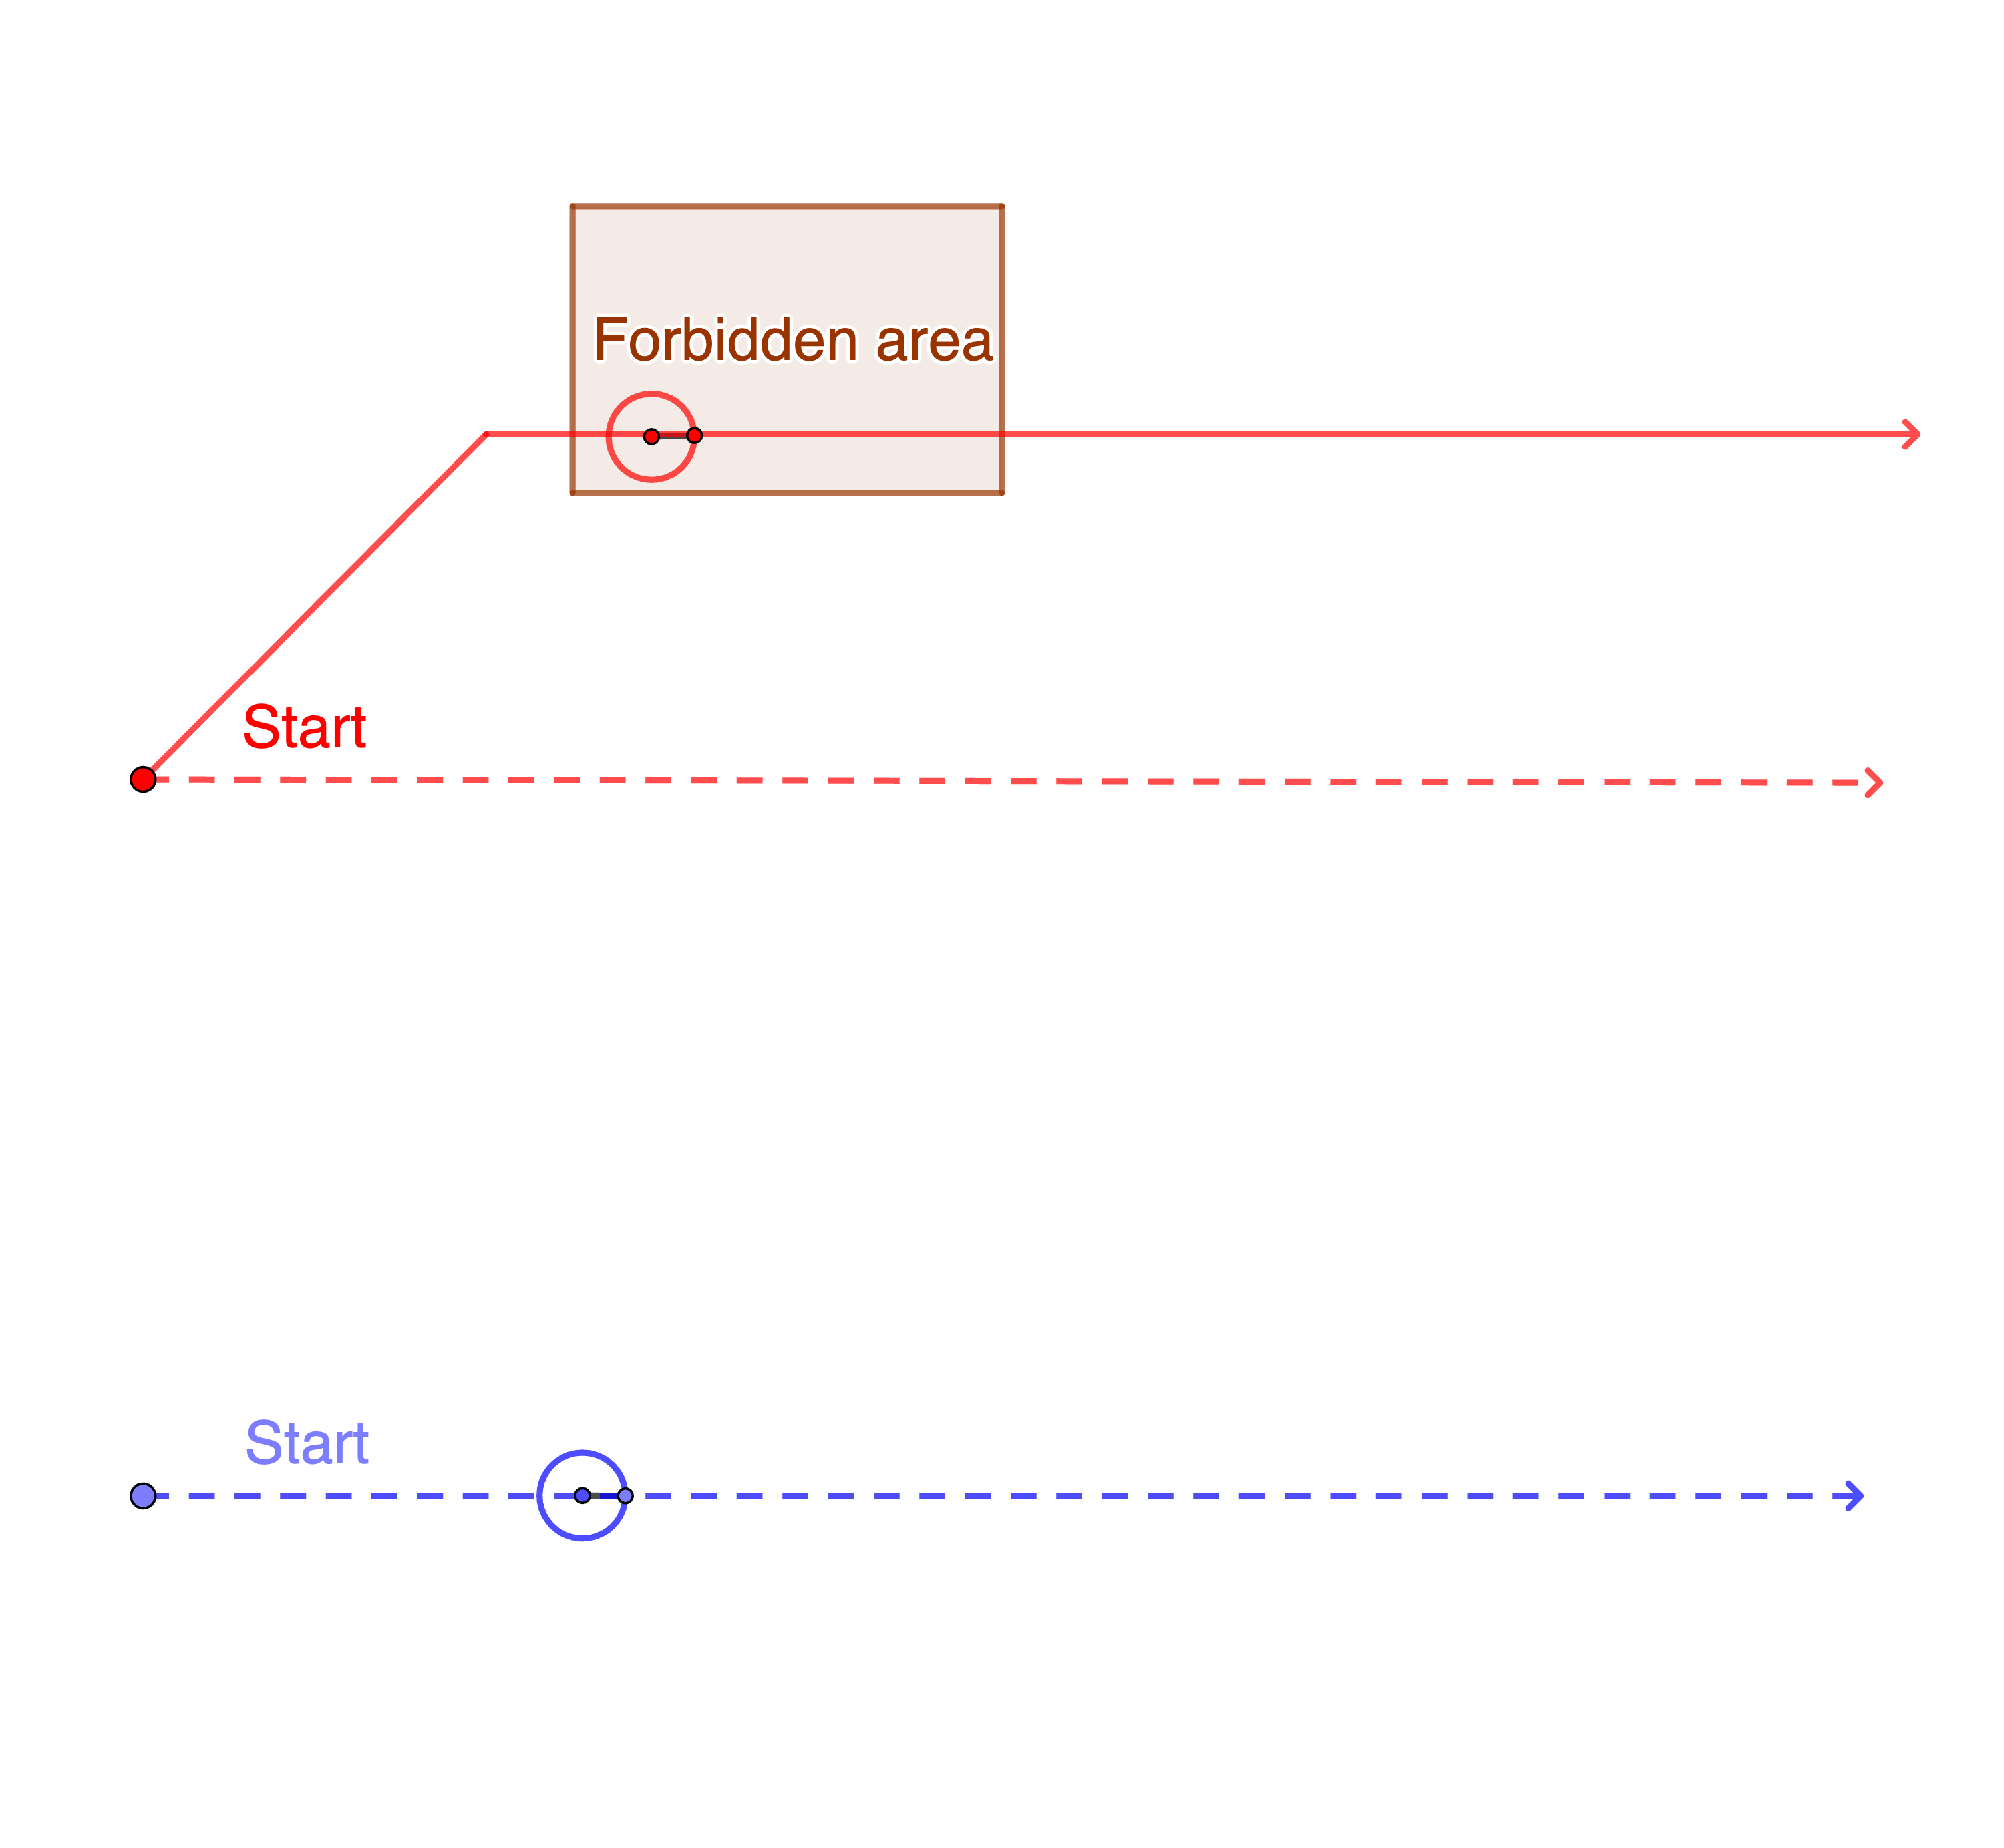
\includegraphics[width = 0.32\linewidth]{plan-deviation}}
    \subfloat[Co-observation \label{fig:example-co-observation}]{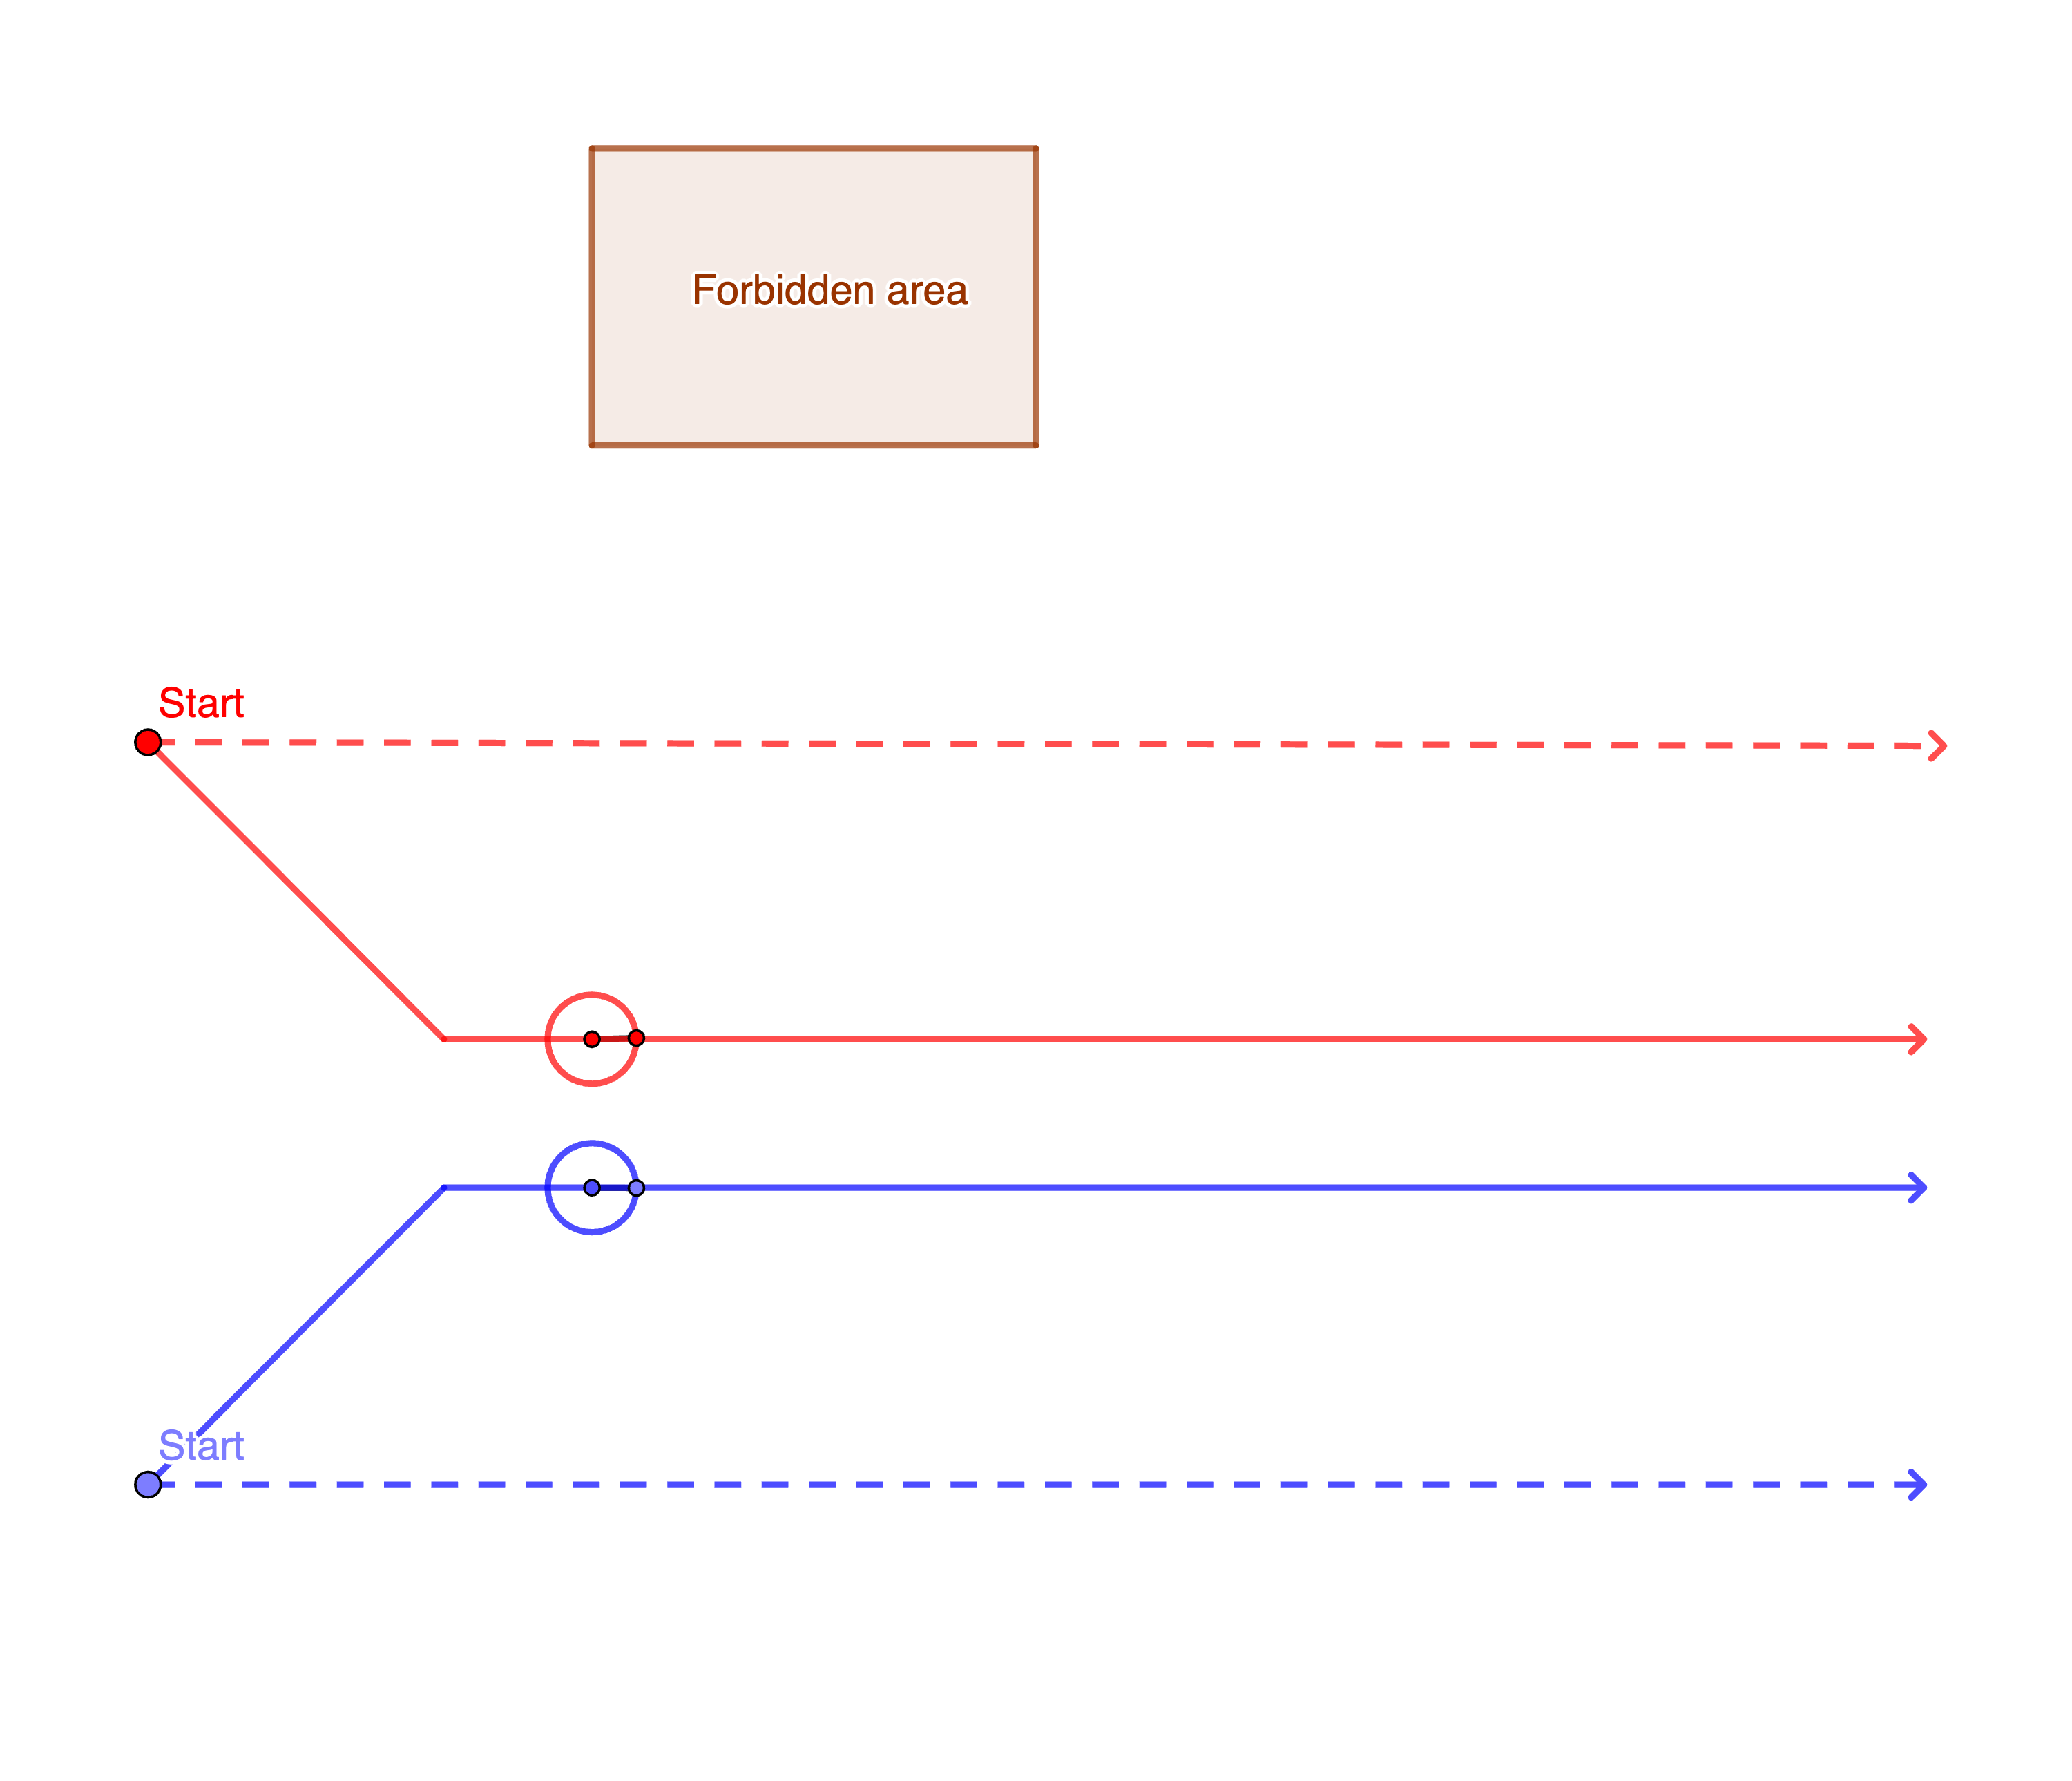
\includegraphics[width=0.32\linewidth]{co-observ}}
    \subfloat[Cross-trajectory co-observation \label{fig:example-cross-traj}]{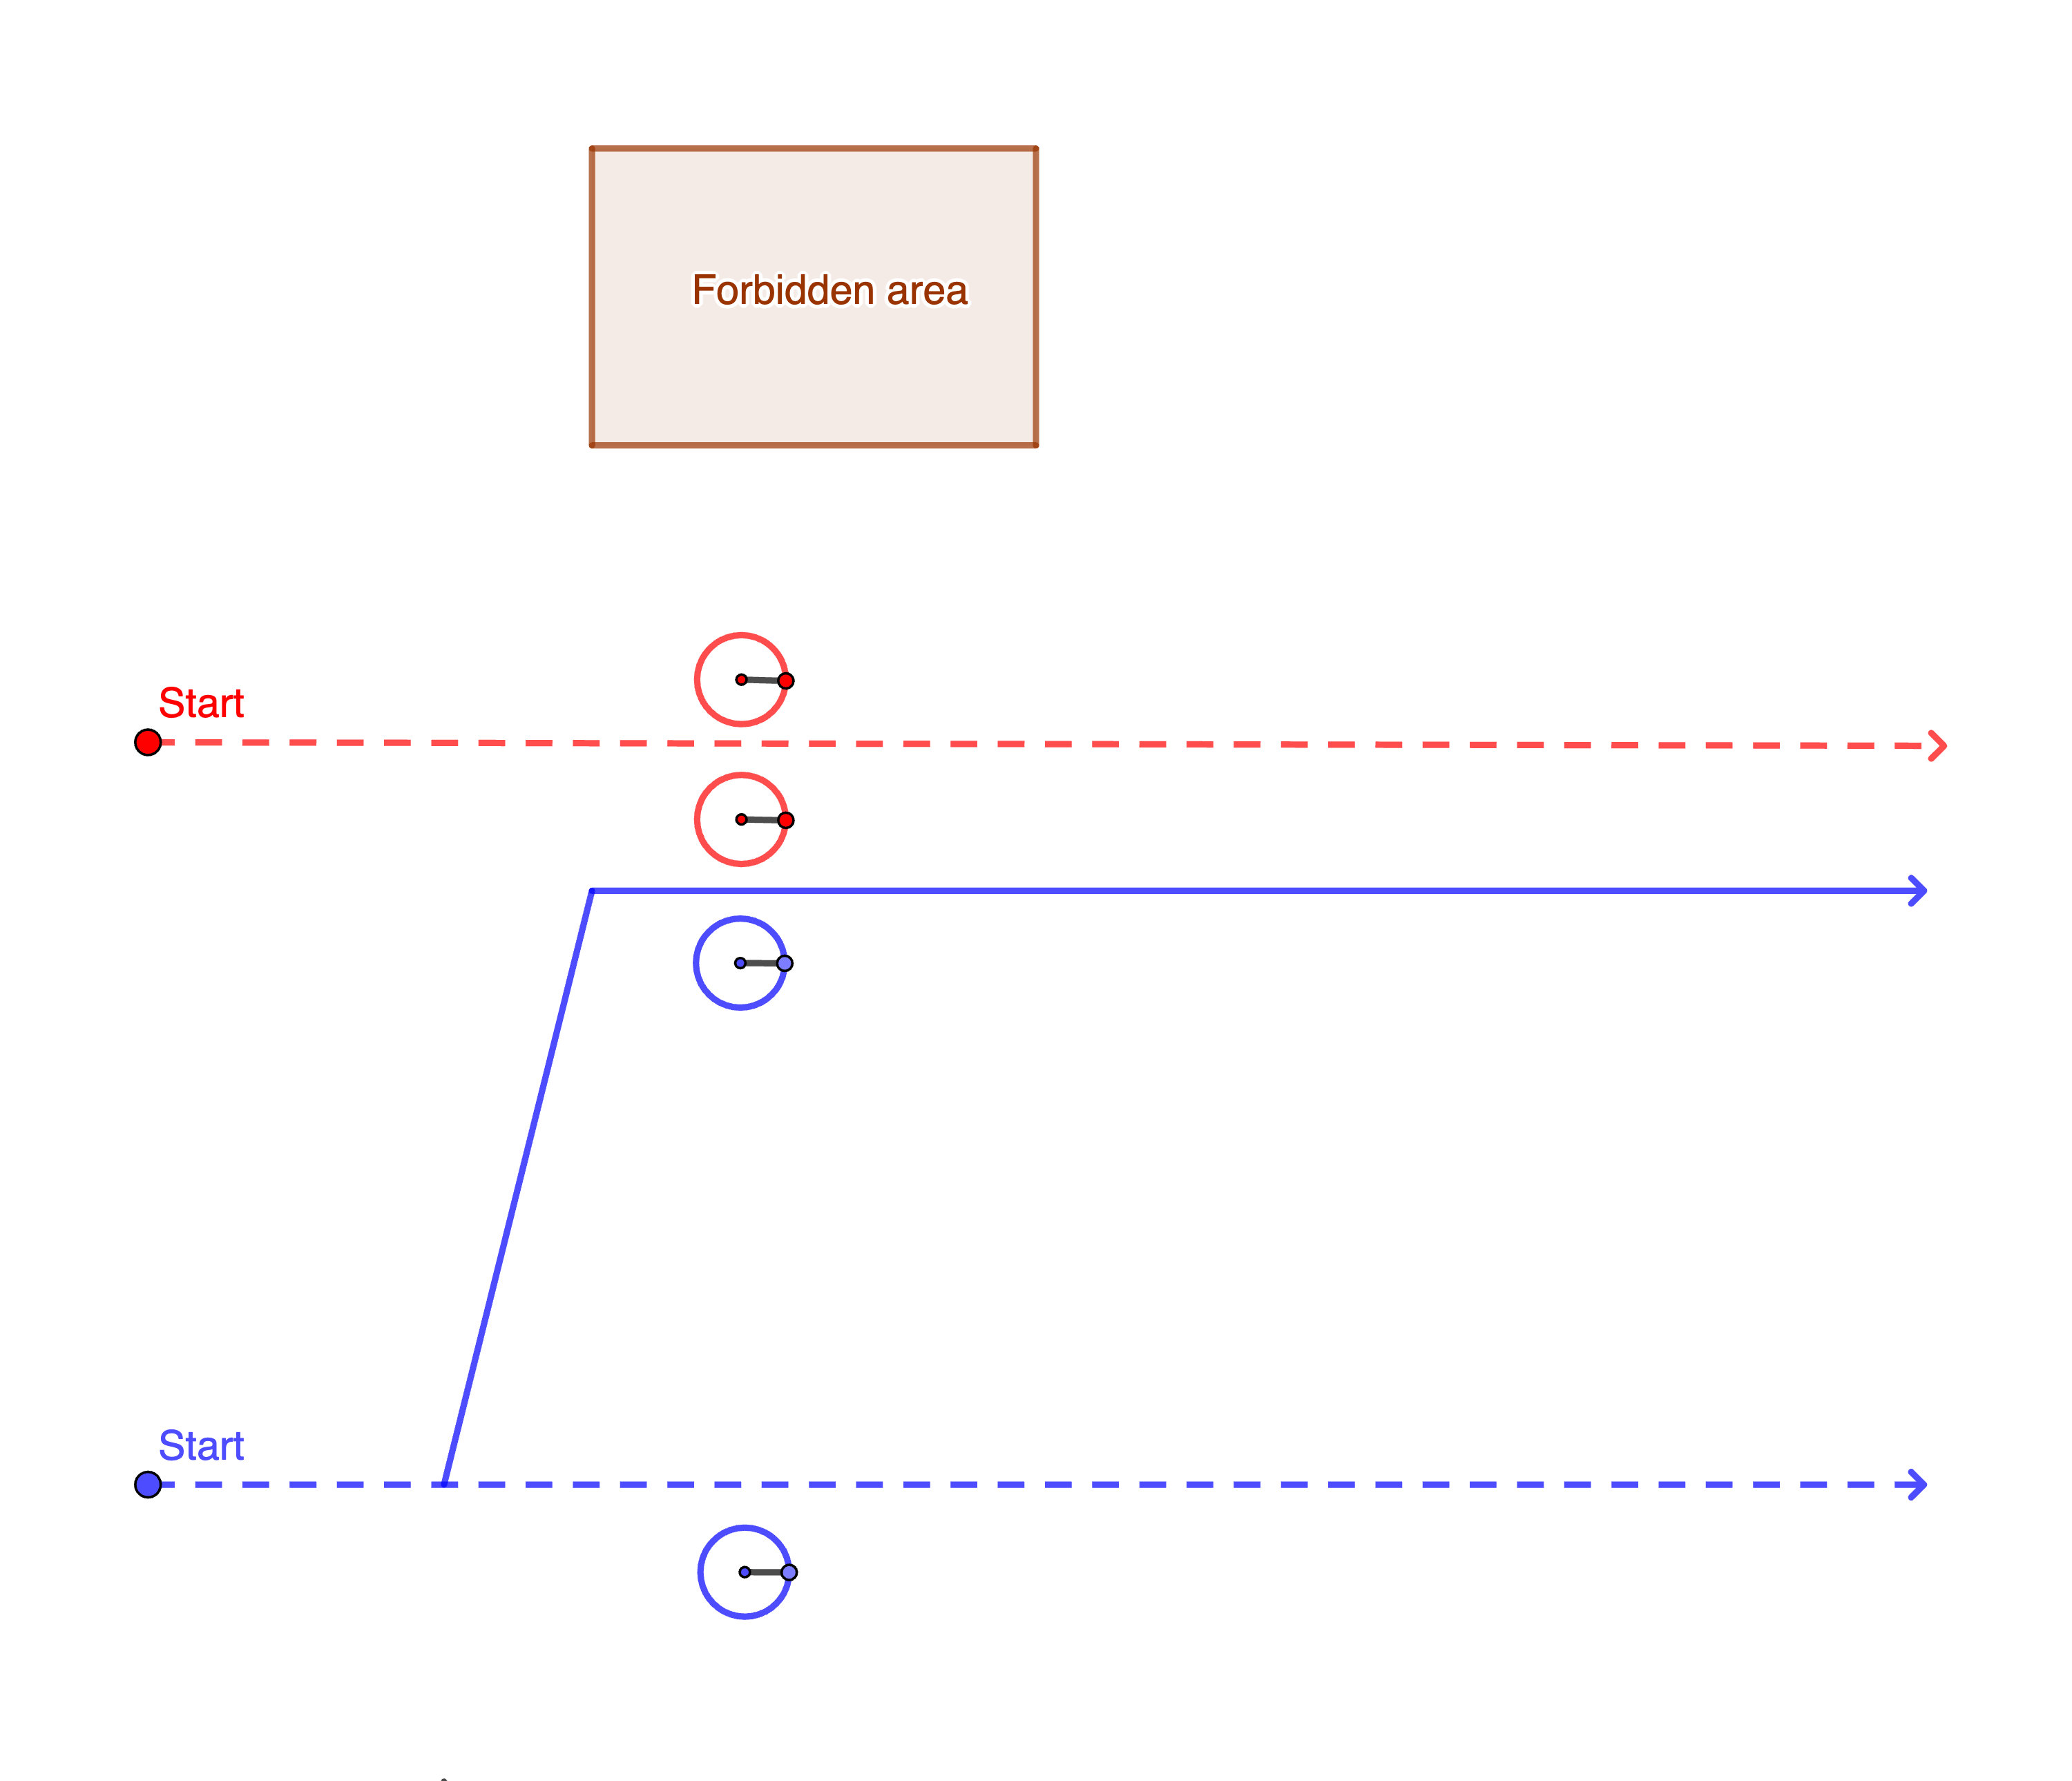
\includegraphics[width=0.32\linewidth]{cross-traj}}
    
    \caption{\ref{fig:example-co-observation} Limited by the co-observation requirement, both red and blue robot follow the co-observation secured routes (solid lines) and abandon the optimal ones (dashed line). \ref{fig:example-cross-traj} Through cross-trajectory co-observations, the blue team sends one robot to follow the red team (solid blue line) and performs co-observation while having the rest of the robots following the optimal trajectory.}\label{fig:cross-traj-comparison-set}
\end{figure}

\noindent\myparagraph{Related research} Trajectory planning problem of MRS systems remained as a subject of intense study for many decades, and optimization is a common approaches in such area. Optimization based approaches are customizable to a variable of constraints (e.g. speed limit, avoid obstacles) and task specifications (e.g. maximum surveillance coverage, minimal energy cost). In constract to our work in \Cref{sec:ADMM-planning}, many motion planning tasks require a non-convex constraint problem formulation, most contributors focused on convex problems, and only allow for a few types of pre-specified non-convex constraints through convexification\cite{liu2014solving}\cite{VanParys2016}\cite{Schulman2014}. Several optimization techniques like MIQP~\cite{mellinger2012mixed} and ADMM~\cite{bento2013message} have been used to reduce computational complexity, and to incorporate more complex non-convex constraints.

Graph-based search is another extensively explored approach in trajectory planning problems, such as formation control \cite{tanner2004leader,hu2019distributed} and Multi-Agent Path Finding (MAPF) problems \cite{stern2019multi}. In traditional MAPF formulations, environments are abstracted as graphs, with nodes representing positions and edges denoting possible transitions between positions and solved as a network flow problem \cite{yu2013multi,yu2016optimal}. This formulation allows for the application of combinatorial network flow algorithms and linear program techniques, offering efficient and more flexible solutions to the planning problem. %In contrast with such approach, our research in \Cref{sec:cross-trajectory} abstracts the existing Multi-Robot System (MRS) trajectory (instead of the environment) into a directed graph and formulates the cross-trajectory co-observation paths as flows.
\rtron{Cite the paper from the reviewer, as well as the paper from Tedrake on the IRIS decomposition, saying that ellipsoids have been used to create approximations of the free configuration space, not to bound reacheability, and not for security application here.}

In \Cref{sec:ADMM-planning}, we incorporate reachability constraints to increase overall security Reachability analysis is a important step in the security and safety verification synthesis for cyber-physical systems (CPSs) \cite{gueguen2009safety,ding2020secure}. One typical approach involves computing an over-approximation of the reachable space for checking safety properities. Previous studies \cite{kurzhanski2000ellipsoidal,lakhal2019interval,maiga2015comprehensive} often use geometric representation, such as zonotopes and ellipsoids, as a compact enclosure of the reachability sets. In the realm of online safety assessment against cyber attacks, \cite{kwon2017reachability} computed the reachable set of CPS states achievable by potential cyber attacks and compared it with the safe region, set based on current state estimation and environmental conditions. 


\noindent\myparagraph{Paper contributions} 
In this paper, two main contributions have been presented. 

\begin{itemize}
  \item We present an innovative method to integrate reachability analysis into the ADMM-based optimal trajectory solver for multi-robot systems, preventing attackers from executing undetected attacks by simultaneously entering forbidden areas and adhering to co-observation schedules.
  \item We introduce additional robots to form \emph{sub-teams} for both intra-sub-team and cross-sub-team co-observations. A new co-observation planning algorithm is formulated that can generate a resilient multi-robot trajectory with a co-observation plan that still preserve the optimal performance against arbitrary tasks. We also find the minimum redundant robots required for the security.
\end{itemize}

\noindent\myparagraph{Paper Outline}
The rest of this paper is organized as follows. In \Cref{sec:ADMM-planning}, we begin by providing an overview of the ADMM-based optimal trajectory solver. We then introduced the ellipsoidal reachability region and formulate it to different constraints with respect to different type of forbidden regions. In \Cref{sec:cross-trajectory}, we proposed the formulation of sub-teams and introduced the planning algorithm of the cross-trajectory co-observation planning problem. Finally, in \Cref{sec:summary}, we provide summary of this paper.

\section{Multi-robot trajectory planning with co-observation}\label{sec:ADMM-planning}

In this section, we design an inter-robot observation plan (co-observation schedule) to ensures that, during the task period, robots are constantly in proximity to one another according to a schedule, in order to observe and detect potential hazardous behaviors. 
This is achieved by keeping the potential region that the robots can possibly reach between each consecutive co-observations away from the forbidden regions. 
\begin{definition}\label{def:secured-plan}
  A multi-robot trajectory plan is secure again plan-deviation attacks if it ensures that any potential deviations to these forbidden regions will cause the corresponding robot to miss their next co-observation with other robots. 
\end{definition}

%This problem is first solved by \cite{wardega2019resilience} in grid world for robots with fixed start and goal locations (Figure~\ref{fig:Grid-example-application}) but does not offer the ability to optimize arbitrary smooth cost functions of the trajectories. 

\rtron{Clarify when we use bold symbols. Make sure this is used consistently.}
We formulate the planning problem as an optimal trajectory optimization problem to minimize arbitrary smooth objective functions. We denote as $q_{ij}\in\real{m}$ the position of agent $i$ at the discrete-time index $j$, with $m$ representing the dimension of the state space. For a total of $n_p$ robots, and a task time horizon of $T$, a total of $n_p$ trajectories can be represented as an aggregated vector $\vq\in \real{n m T}$. 
The overall goal is to minimize or maximize an objective function $\varPhi(\vq)$ under a set of nonlinear constraints described by a set $\Omega$, which is given by the intersection of spatio-temporal sets given by traditional path planning constraintsand the security constraints (co-observation schedule, reachability analysis). Formally:
\begin{equation}\label{eq:general-problem}
	\begin{split}
		\min/\max & \quad \varPhi(\vq)\\
		\textrm{subject to} &\quad \vq \in \Omega.
	\end{split}
\end{equation}

To give a concrete example of the cost $\varPhi$ and the set $\Omega$, we introduce a representative application that will be used for all the simulations throughout the paper.

\begin{example} 
Robots are tasked to navigate, collecting sensory data to construct a corresponding map for the slowly-varying field, denoted as $\vx$, of an unknown environment (see Figure~\ref{fig:SecurityBreak}). The map comprises points of interest arranged on a grid, each associated with a slowly-changing value. Our goal is to find paths that minimize uncertainty and effectively reconstruct the field. 
We associate a Kalman Filter (KF)~(cf. \cite{anderson2012optimal}) to each point $j$, and use it to track the uncertainty through its estimated covariance $P_j$. The updates of the filters are based on measurements from the robot centered at $q$, and we use a Gaussian radial basis function  modeling spatially-varying measurement quality. The optimization objective $\varPhi(\vq)$ is written as the maximum uncertainty $\max_j P_{j}$ (detailed formulation can be found in \cite{yang2020multi}). %The set $\Omega$ includes traditional constraints like bounded velocity, convex obstacles, waypoints to reach with deadlines, in addition to security constraints including co-observation and reachability constraints.
\rtron{Relate to Fig. 2}
\end{example}

\begin{figure}
     \centering
     \subfloat[Grid-world trajectory. \label{fig:Grid-example-application}]{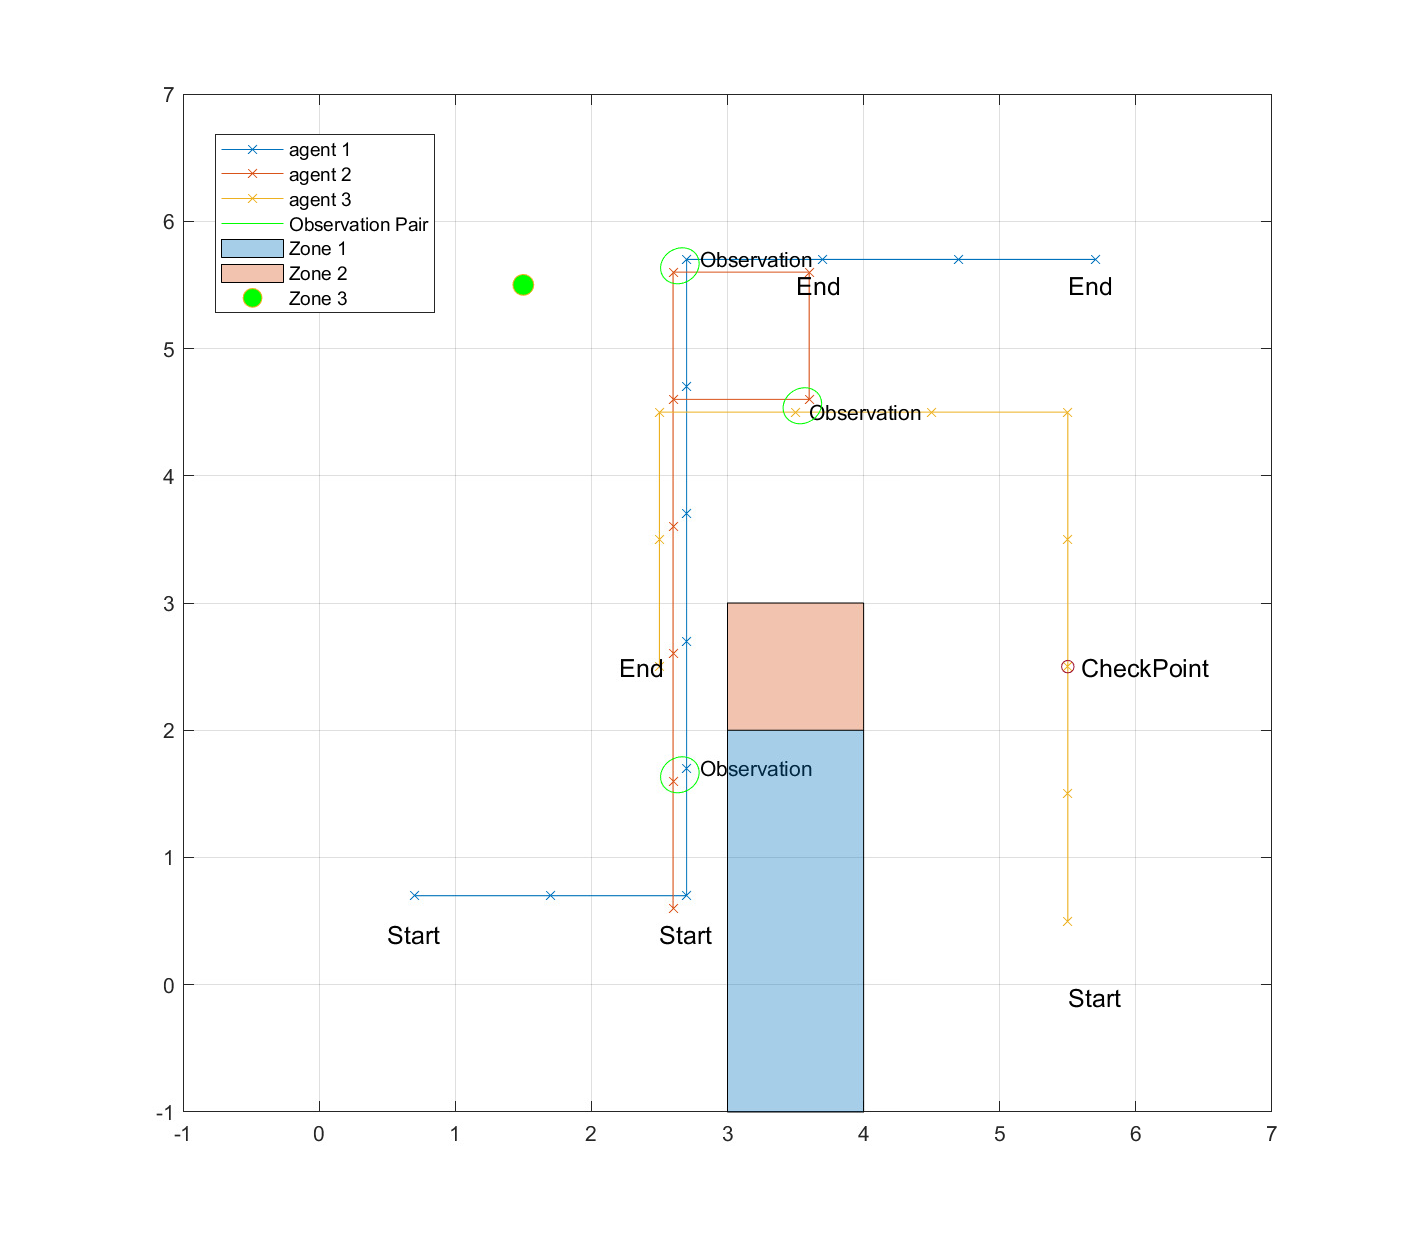
\includegraphics[width=0.45\linewidth, trim = 2cm 0.5cm 0cm 2cm]{Kacper_result}}
     \subfloat[Continuous world trajectory \label{fig:SecurityBreak}]{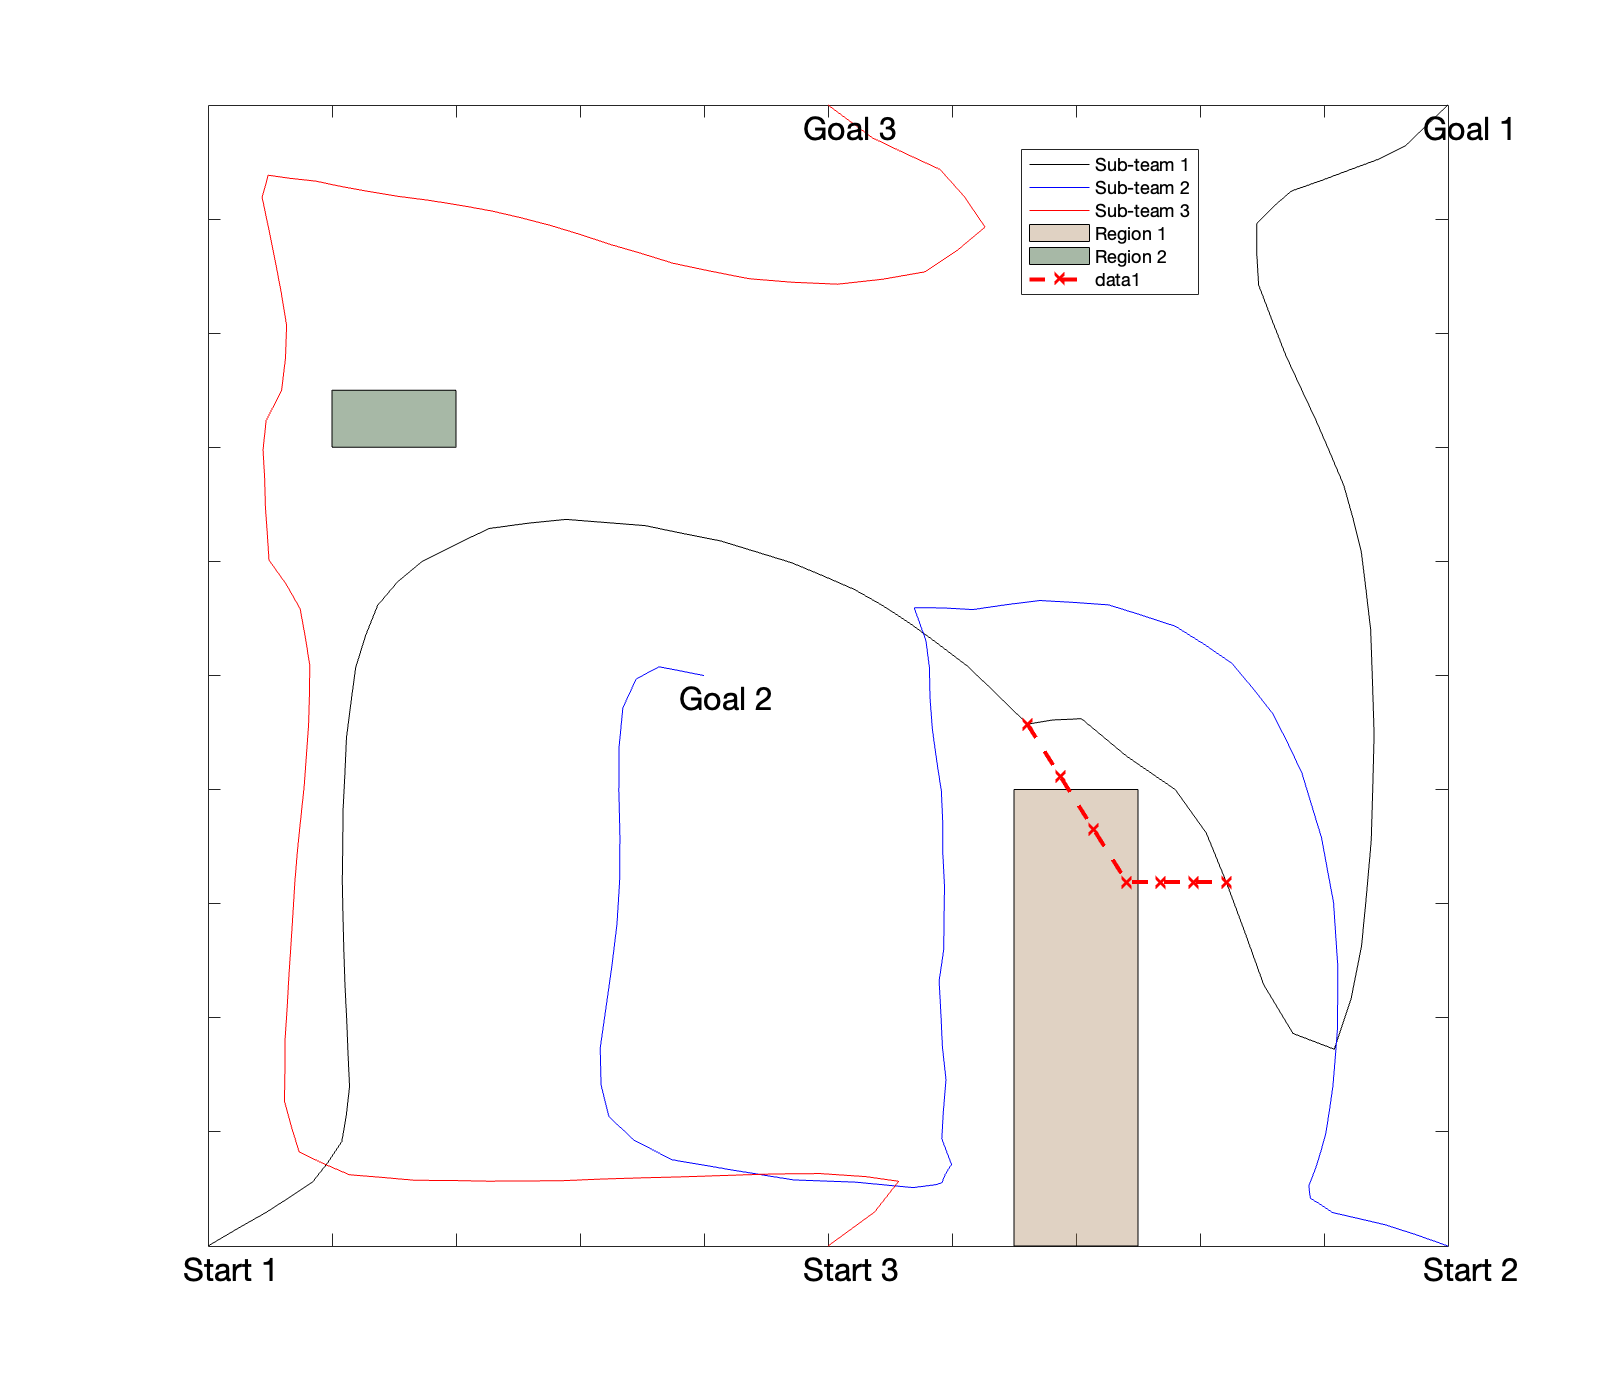
\includegraphics[width=0.45\linewidth, trim = 2cm 2cm 2cm 2cm]{SecurityBreak}}
     \caption{Trajectory design of an example map exploration task for a three-robot system with start locations and destinations fixed. Task are planned in a $8 \times 8$ grid world. Zone 1 is obstacle, Zone 2 and Zone 3 are safe zones. Fig~\ref{fig:Grid-example-application} shows the planned trajectory with co-observation schedule in grid-world. Fig~\ref{fig:SecurityBreak} shows the unsecured trajectory design in continuous world optimized with respect to a map exploration task where Zone 1 and 2 are considered together as one obstacle.  A potential path that could break the security by entering region 1 is highlighted in dashline.}
     \label{fig:example-application}
 \end{figure}

% This section is organized as follows. We begin with foundational mathematical concepts needed for the optimal trajectory solver and reachability constraints. Subsequently, we integrate security constraints, including co-observation schedule and reachability constraints. Finally, we present the obtained results alongside limitations that are then addressed in \Cref{sec:cross-trajectory}.

\subsection{Preliminaries}
\subsubsection{Differentials}
We define the differential of a map $f(x):\real{m}\to\real{n}$ at a point $x_0$ as the unique matrix $\partial_x f \in\real{n\times m}$ such that
\begin{equation}\label{equ:dt_to_dx}
  \left.\dert f\bigl(x(t)\bigr)\right|_{t=0}=\partial_x f\bigl(x(0)\bigr) \dot{x}(0)
\end{equation}
where $t\mapsto x(t)\in\real{n}$ is a smooth parametric curve such that $x(0)=x$ with any arbitrary tangent $\dot{x}(0)$. For brevity we will use $\dot f$ for $\dert f$ and $\partial_x f$ for $\frac{\partial f}{\partial x}$. 
%The differentials $\partial_x f$ is derived through \eqref{equ:dt_to_dx} having $\dot f$ divided by $\dot x$.

With a slight abuse of notation, we use the same notation $\partial_xf$ for the differential of a matrix-valued function with scalar arguments $f:\real{R}\to\real{m\times n}$.  Note that in this case \eqref{equ:dt_to_dx} is still formally correct, although the RHS needs to be interpreted as applying $\partial_x f$ as a linear operator to $\dot{x}$.

 \subsubsection{Householder rotations}\label{sec:householder}
  We define a differentiable transformation to a canonical ellipse that is used in the derivation of the reachability constraints in \Cref{sec:reachability,sec:ellipse-region-constraint}. This transformation includes a rotation derived from a modified version of Householder transformations \cite{householder1958unitary}. With respect to the standard definition, our modification ensures that the final operator is a proper rotation (i.e., not a reflection). We call our version of the operator a \emph{Householder rotation}. In this section we derive Householder rotations and their differentials for the 3-D case; the 2-D case can be easily obtained by embedding it in the $z=0$ plane.

  \begin{definition} Let $\nu_\cF$ and $\nu_\cE$ be two unitary vectors ($\norm{\nu_\cF}=\norm{\nu_\cE}=1$). \rtron{Add the explicit dependency of $u$, $u'$ on $\nu_F,\nu_E$.} Define the normalized vector $u$ as
    \begin{equation}
      u'=\nu_\cF+\nu_\cE,\quad u =\frac{u'}{\norm{u'}}.
    \end{equation}
    The \emph{Householder rotation} $H(\nu_\cF,\nu_\cE)$ is defined as
    \begin{equation}\label{eq:H definition}
      H(\nu_\cF,\nu_\cE) = 2 u u\transpose-I.
    \end{equation}
  \end{definition}
  Here $H$ is a rotation mapping \rtronhl{Remove hats}{$\hat{\nu_\cF}$ to $\hat{\nu_\cE}$}, as shown by the following.
  \begin{proposition}\label{prop:HProperty}
    The matrix $H$ has the following properties:
    \begin{enumerate}
    \item It is a rotation, i.e.
      \begin{enumerate}
      \item\label{it:orthonormality} $H\transpose H=I$;
      \item\label{it:determinant} $\det(H)=1$.
      \end{enumerate}
    \item\label{it:transformation} $\nu_\cE=H \nu_\cF$.
    \end{enumerate}
  \end{proposition}
  \begin{proof}
  	See Appendix \ref{proof:HProperty}.
  \end{proof}

  We compute the differential of $H$ implicitly using its definition \eqref{equ:dt_to_dx}. We use the notation $\cross{v}:\real{3}\to\real{3\times 3}$ to denote the matrix representation of the cross product with the vector $v$, i.e.,
  \begin{equation}
    \bmat{v_1\\v_2\\v_3}_\times= \bmat{0 & -v_3 &v_2\\v_3 & 0 & -v_1\\-v_2 & v_1 & 0},
  \end{equation}
  such that $[v]_\times w=v\times w$ for any $w\in\real{3}$. %One can verify by direct computation the following property:
  %\begin{equation}\label{eq:asymmetric to cross}
  %  wv\transpose-vw\transpose=\cross{\cross{v}w}.
  %\end{equation}
  \begin{proposition}\label{prop:Hderivitive}
    Let $\nu_\cF(t)$ represent a parametric curve. Then
    \begin{equation}
      \dot{H}=H\cross{-2M\dot{\nu}_{\cF}},
    \end{equation}
    where the matrix $M\in\real{3\times3}$ is given by
    \begin{equation}
      M=[u]_{\times}  \frac{ \left( I - u u\transpose \right) \left( I- \nu_\cF \nu_\cF\transpose \right)} {\norm{u'} \norm{\nu_\cF}}.
    \end{equation}
  \end{proposition}
  \begin{proof}
  	See Appendix \ref{proof:Hderivitive}.
  \end{proof}

\subsubsection{Alternating Directions Method of Multipliers (ADMM)}\label{chapter:ADMM review}
The basic idea of the ADMM-based solver introduced in \cite{yang2020multi} is to separate the constraints from the objective function using a different set of variables $\vz$, and then solve separately in \eqref{eq:general-problem}.
More specifically, we rewrite the constraint $\vq\in\varOmega$ using an indicator function $\varTheta$, and include it in the objective function (details can be found in \cite{yang2020multi}). 
%In the traditional application of ADMM, the variables $\vz$ are simple duplicates of $\vx$ projected to the constraint set $\Omega$. However, in path planning problems, some constraints are non-convex, rendering the projection step more difficult (due to the presence of multiple local minima).
We allow $\vz = D(\vq)$ to replicate an arbitrary function of the main variables $\vq$ (instead of being an exact copy in general ADMM formulation), to transform constraint $\vq\in\Omega$ to $D(\vq) \in \sZ$ to allow for an easier projection step in \Cref{eq:z-update}. In summary, we transform \Cref{eq:general-problem} into
\begin{equation}\label{eq:ADMMSetConstraint_modified}
	\begin{aligned}
		&\max\quad \varPhi(\vq)+\varTheta(\vz) \\
		& \begin{array}{r@{\quad}c}
			s.t.& D(\vq)-\vz=0
		\end{array} 
	\end{aligned}
\end{equation}
where $D(\vq)= [D_1(\vq)^T,\dots,D_l(\vq)^T]^T$ is a vertical concatenation of different functions for different constraints. This makes each constraint set $\mathcal{Z}_i$ independent and thus can be computed separately in later updating steps. $D_i(\vq)$ is chosen that the new constraint set~$\cZ_i$ becomes simple to compute which is illustrated in later secitons. % and the function~$D_i(\vq)$ can be used to select only the subset of the variables on which a constraint depends, speeding up computations.

The update steps of the algorithm are then derived as \cite{Boyd2011}:
\begin{subequations}\label{eq:ADMMupdate}
	\begin{align}
		\label{eq:admm-mod-update-q}\vq^{k+1}&:=\argmin_\vq(\varPhi(\vq^k) +\frac{\rho}{2}\norm{D(\vq)-\vz^k+\vu^k}_2^2),\\
		\vz^{k+1}&:=\Pi_\mathcal{Z}(D(\vq^{k+1})+\vu^k), \label{eq:z-update} \\
		\vu^{k+1}&:=\vu^k+D(\vq^{k+1})-\vz^{k+1},
	\end{align}
\end{subequations}
where $\Pi_\mathcal{Z}$ is the new projection function to the modified constraint set $\mathcal{Z}$, $\vu$ represents a scaled dual variable that, intuitively, accumulates the sum of primal residuals
\begin{equation}\label{eq:primal-residual}
	\vr^{k}=D(\vq^{k+1})-\vz^{k+1}.
\end{equation}
Checking the primal residuals alongside with the dual residuals 
\begin{equation}\label{eq:dual-residual}
	\vs^{k}=-\rho(\vz^{k}-\vz^{k-1})
\end{equation}
after each iteration, the steps are reiterated until convergence when the primal and dual residuals are small, or divergence when primal and dual residual remains large after a fixed number of iterations.
\rtron{Maybe state here that (9a) is solved iteratively, while (9b) and (9c) are closed-form.}

We now provide the functions $D(\vq)$, the sets $\cZ$, and the corresponding projection operators $\Pi_\cZ$ for security constraints including co-observation security constraints (\Cref{sec:co-observation-constraint}), and reachability constraints (\Cref{sec:ellipsoid-point}-\Cref{eq:region_ellipsoid_constraint}). The latter are based on the definition of \emph{ellipse-region-constraint} (\Cref{sec:reachability}).
Formulation of traditional path planning constraints like velocity constraints, convex obstacle constraints can be found in \cite{yang2020multi}.

% \subsection{Velocity constraints}\label{sec:velocity-constraint}
% We constraint for the movement of each agent by a maximum velocity defined as the distance in any direction over a single discrete time step. The function $D(\vq)$ returns the velocity vectors for the $i$-th agent at each time step $j$, and constrain its result to a sphere.
% \begin{constraint}[Velocity constraint]
% \begin{align}
%      D_{ij}(\vq) &= q_{ij}-q_{i(j-1)}, \quad j\in\{1,\ldots, T\},\\
% \label{eq:velocity_constraint}
%    \sZ_{ij} &=\bigl\{\vz \mid \norm{\vz} \leq v_{max}\bigr\},\\
%    \Pi_{\sZ_{ij}}(\vz)&=\begin{cases}
%    v_{\max}\frac{\vz}{\norm{\vz}} \textrm{ if } \norm{\vz}>v_{\max},\\
%    \vz\textrm{ otherwise.}
%    \end{cases}
% \end{align}
% \end{constraint}

% \subsection{Convex polygonal obstacles collision constraints} \label{sec:obstacle-constraint}
% We use convex polygons $\cP$ to model regions  that cannot be entered by agents (solid obstacles and forbidden regions). $\cP$ is defined using a collection of $l$ hyperplanes $n_{k}\transpose q = m_{k}$, where $n_k$ is the normal vector pointing toward the outside of the obstacle and $m_k$ is the scalar offset defining the $k$-th hyperplane.We define the function $D(\vq)$ to return the maximum distance from $q_{ij}$ to all hyperplane boundaries of region $\cP$, and  constraint $z$ to be a non-negative scalar. This constraint is applied to all $q_{ij} \in \vq$. 

% Non-convex obstacles can be handled by a union of (possibly overlapping) convex obstacles. And by using outward-pointing normals for $n_k$, this method can also serve to constrain the robots within a designated workspace region.
% \begin{constraint}[Obstacle constraint]
% \begin{align}
%      	D(q_{ij}) &= \max_{k=1,\dots,l} (d_{k}(q_{ij},\cP)),\\
% \label{eq:obstacle_constraint}
%   \sZ &= \{z \mid z \geq 0 \},\\
%    \Pi_\sZ(z) & = \begin{cases}
%    0 & \textrm{if} \quad z < 0,\\
%    z  & \textrm{otherwise.}
%    \end{cases} \label{eq:zoneConstraintProjection}
% \end{align}
% where $d_{k}(q_{ij},\cP)= p_{ij}\transpose n_k - m_k$ returns the distance between a single waypoint $q_{ij}$ and the $k$th hyperplane .
% \end{constraint}
% %The motivating idea for \eqref{eq:obstacle_constraint} and \eqref{eq:zoneConstraintProjection} is to identify waypoints within a specific region and project them to the closest boundary. 

% \subsection{Waypoints with flexible deadlines}\label{sec:waypoint-constraint}
% Security-related constraints often necessitate that a robot reaches a specified location at a particular time. We assume that robot $i$ is tasked with reaching a given point $p$ within a radius of $d_{max}$ at some time instant $j$ within a predefined time window $[t_1,t_2]$, leading to the following:

% \begin{constraint}[Waypoint constraint]
% \begin{align}
%      	D(\vq) &= \min_{j\in\{t_1,\dots,t_2-1\}}\bigl(\dist(p,\overrightarrow{q_{ij}q_{i(j+1)}})\bigr),\\
% \label{eq:waypoint_constraint}
%   \sZ &= \{z \mid z < z_{max} \},\\
%    \Pi_\sZ(z) & = \min(z, d_{max}),
% \end{align}
% where $\dist(p,\overrightarrow{q_{ij}q_{i(j+1)}})$ returns the distance between the fixed point $p$ and the segment $\overrightarrow{q_{ij}q_{i(j+1)}}$.
% \end{constraint}

% This function returns the smallest distance between $(p,q_{ij})$ and $(p,q_{i(j+1)})$ if the projection of the point $p$ does not lie on the line segment~$\overrightarrow{q_{ij}q_{i(j+1)}}$; as a consequence, this constraint does not need to be satisfied exactly at one of the points on the discretized trajectory, but it can also be satisfied ``en route'' on the segment between them.

\subsection{Co-observation schedule constraint}\label{sec:co-observation-constraint}
The co-observation constraint ensures that two robots come into close proximity at scheduled times to observe each other's behavior. This constraint is represented as a relative distance requirement between the two robots at a specific time instant, ensuring they are within a defined radius to inspect each other or exchange data. %Importantly, the co-observation locations must be chosen to guarantee that the ellipsoidal reachability regions, as discussed in \Cref{sec:reachability}, do not intersect with any forbidden regions.

%The co-observation constraints is used to guarantee that, at time required by the schedule, two robots should get close enough with each other to observe each other's behavior. This constraint is modeled as a relative distance constraint between two robots at some time instant $j$ (i.e., to require two agents see each other within a certain radius to inspect each other, or to exchange data). The location of the co-observation should make sure that the ellipsoidal reachability region between each co-observation, considered in later sections \ref{sec:reachability}, has an empty intersection with all forbidden regions.

% We write the function for the constraint as:
\begin{constraint}[Co-observation constraint]\label{constraint:coobservation}
\begin{align}
D(\vq) &= \overrightarrow{q_{aj}q_{bj}}, \label{eq:coobservation_constraint}\\
  \sZ &= \{\vz \mid \norm{\vz} \leq d_{max} \},\\
   \Pi_\sZ(z) & = \begin{cases}
d_{max}\frac{\vz}{\norm{\vz}} &\text{if } \norm{\vz} > d_{max},\\
\vz	& otherwise,
\end{cases}
\end{align}
where $a,b$ are the indices of the pair of agents required for a mutual inspection.
\end{constraint}
The locations $q_{aj}$ and $q_{bj}$ where the co-observation is performed are computed as part of the optimization.

\subsection{Definition of ellipsoidal reachability regions}\label{sec:reachability}
In this section, we define \emph{ellipsoidal reachability regions} based on pairs of co-observation locations on a trajectory, and a transformation of such region in axis-aligned form. Different types of reachability constraints (between an ellipsoid and different geometric entities such as a point, line, line segment, and polygon) alongside their projections, and differentials are introduced in subsequent sections. Together with the co-observation constraint~\ref{constraint:coobservation}, these will be used in the ADMM formulation of \cref{chapter:ADMM review} to provide security for all observed and unobservered periods.

%The reachability region is defined as the set of locations $q(t)$ that a robot can reach between two given fixed positions:

\begin{definition}\label{sec:ellipsoidal definition}
	The \emph{reachability region} for two waypoints $q(t_1)=q_1$, $q(t_2)=q_2$ is defined as the sets of points $q'$ in the \rtronhl{free configuration space}{workspace} such that there exist a \rtronhl{this $q$ should be probably $q_{dev}$ or something similar, to distinguish it from the planned $q$}{trajectory $q(t)$ where $q(t')=q'$, $t_1\leq t' \leq t_2$ and $q(t)$ satisfies the velocity constraint $d(q(t),q(t+1))\leq v_{max}$}\rtron{, where $d(\cdot,\cdot)$ represents the distance between two points}. 
\end{definition}
This region can be analytically bounded via an ellipsoid:
\begin{definition}\label{def:Reachability}
	The \emph{reachability ellipsoid $\cE$} is defined as the region  $\mathcal{E}(q_1,q_2,t_{1},t_{2})=\{\tilde{q}\in\mathbb{R}^n: d(q_1,\tilde{q})+d(\tilde{q}+q_2)<2a\}$, where $a=\frac{v_{max}}{2}(t_2-t_1)$.
\end{definition}

 \begin{figure}
    \centering
    \subfloat[Showcase of a reachability region\label{fig:EllipseConstraintExample}]{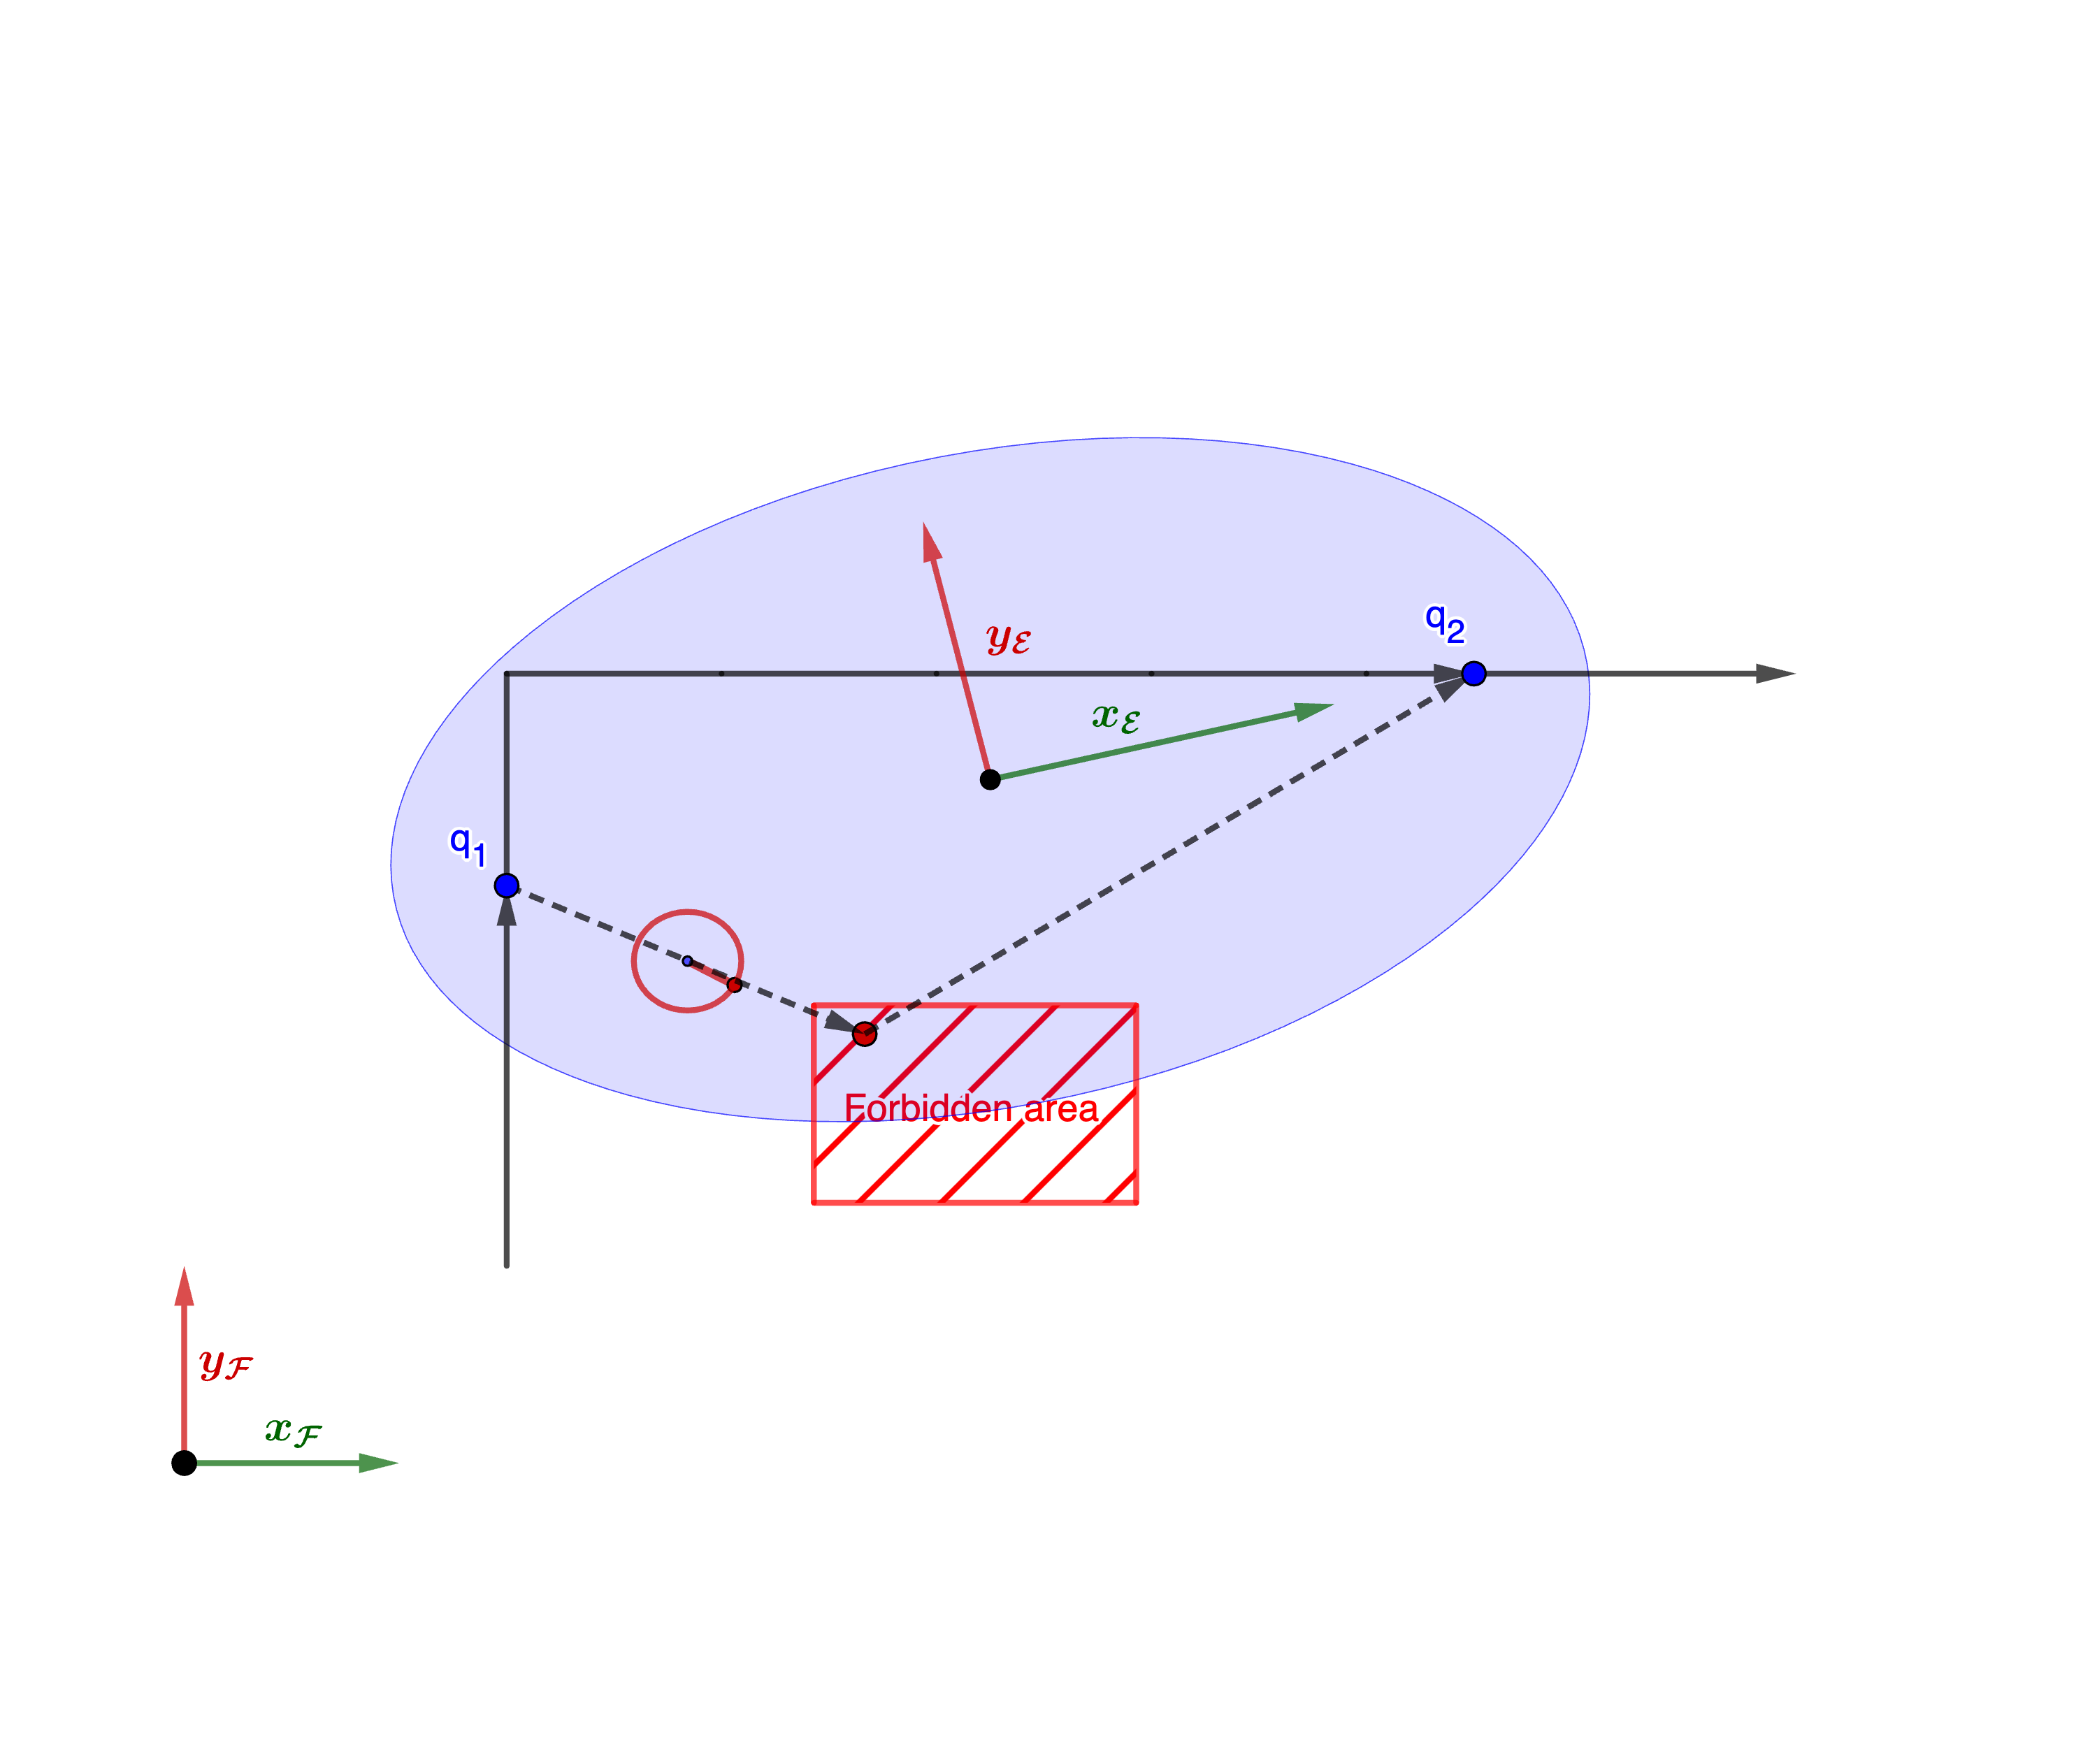
\includegraphics[width=0.47\linewidth, trim = 2cm 2.5cm 2cm 5cm]{Reachability}}
    \subfloat[Point-ellipsoid constraint \label{fig:Ellipse-to-point}]{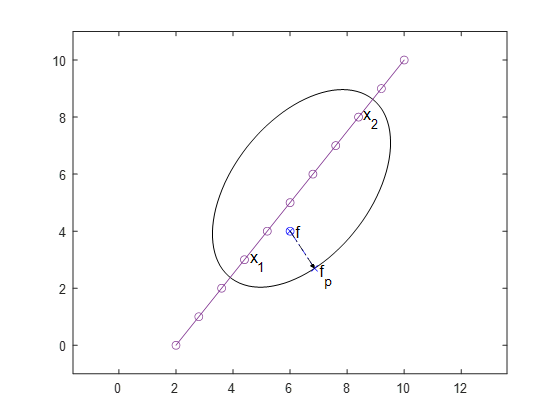
\includegraphics[width=0.47\linewidth, trim = 0.3cm 1.3cm 0.3cm 1.3cm, clip]{Ellipse2point}}

    \subfloat[Plane-ellipse constraint \label{fig:Ellipse-to-plane}]{ 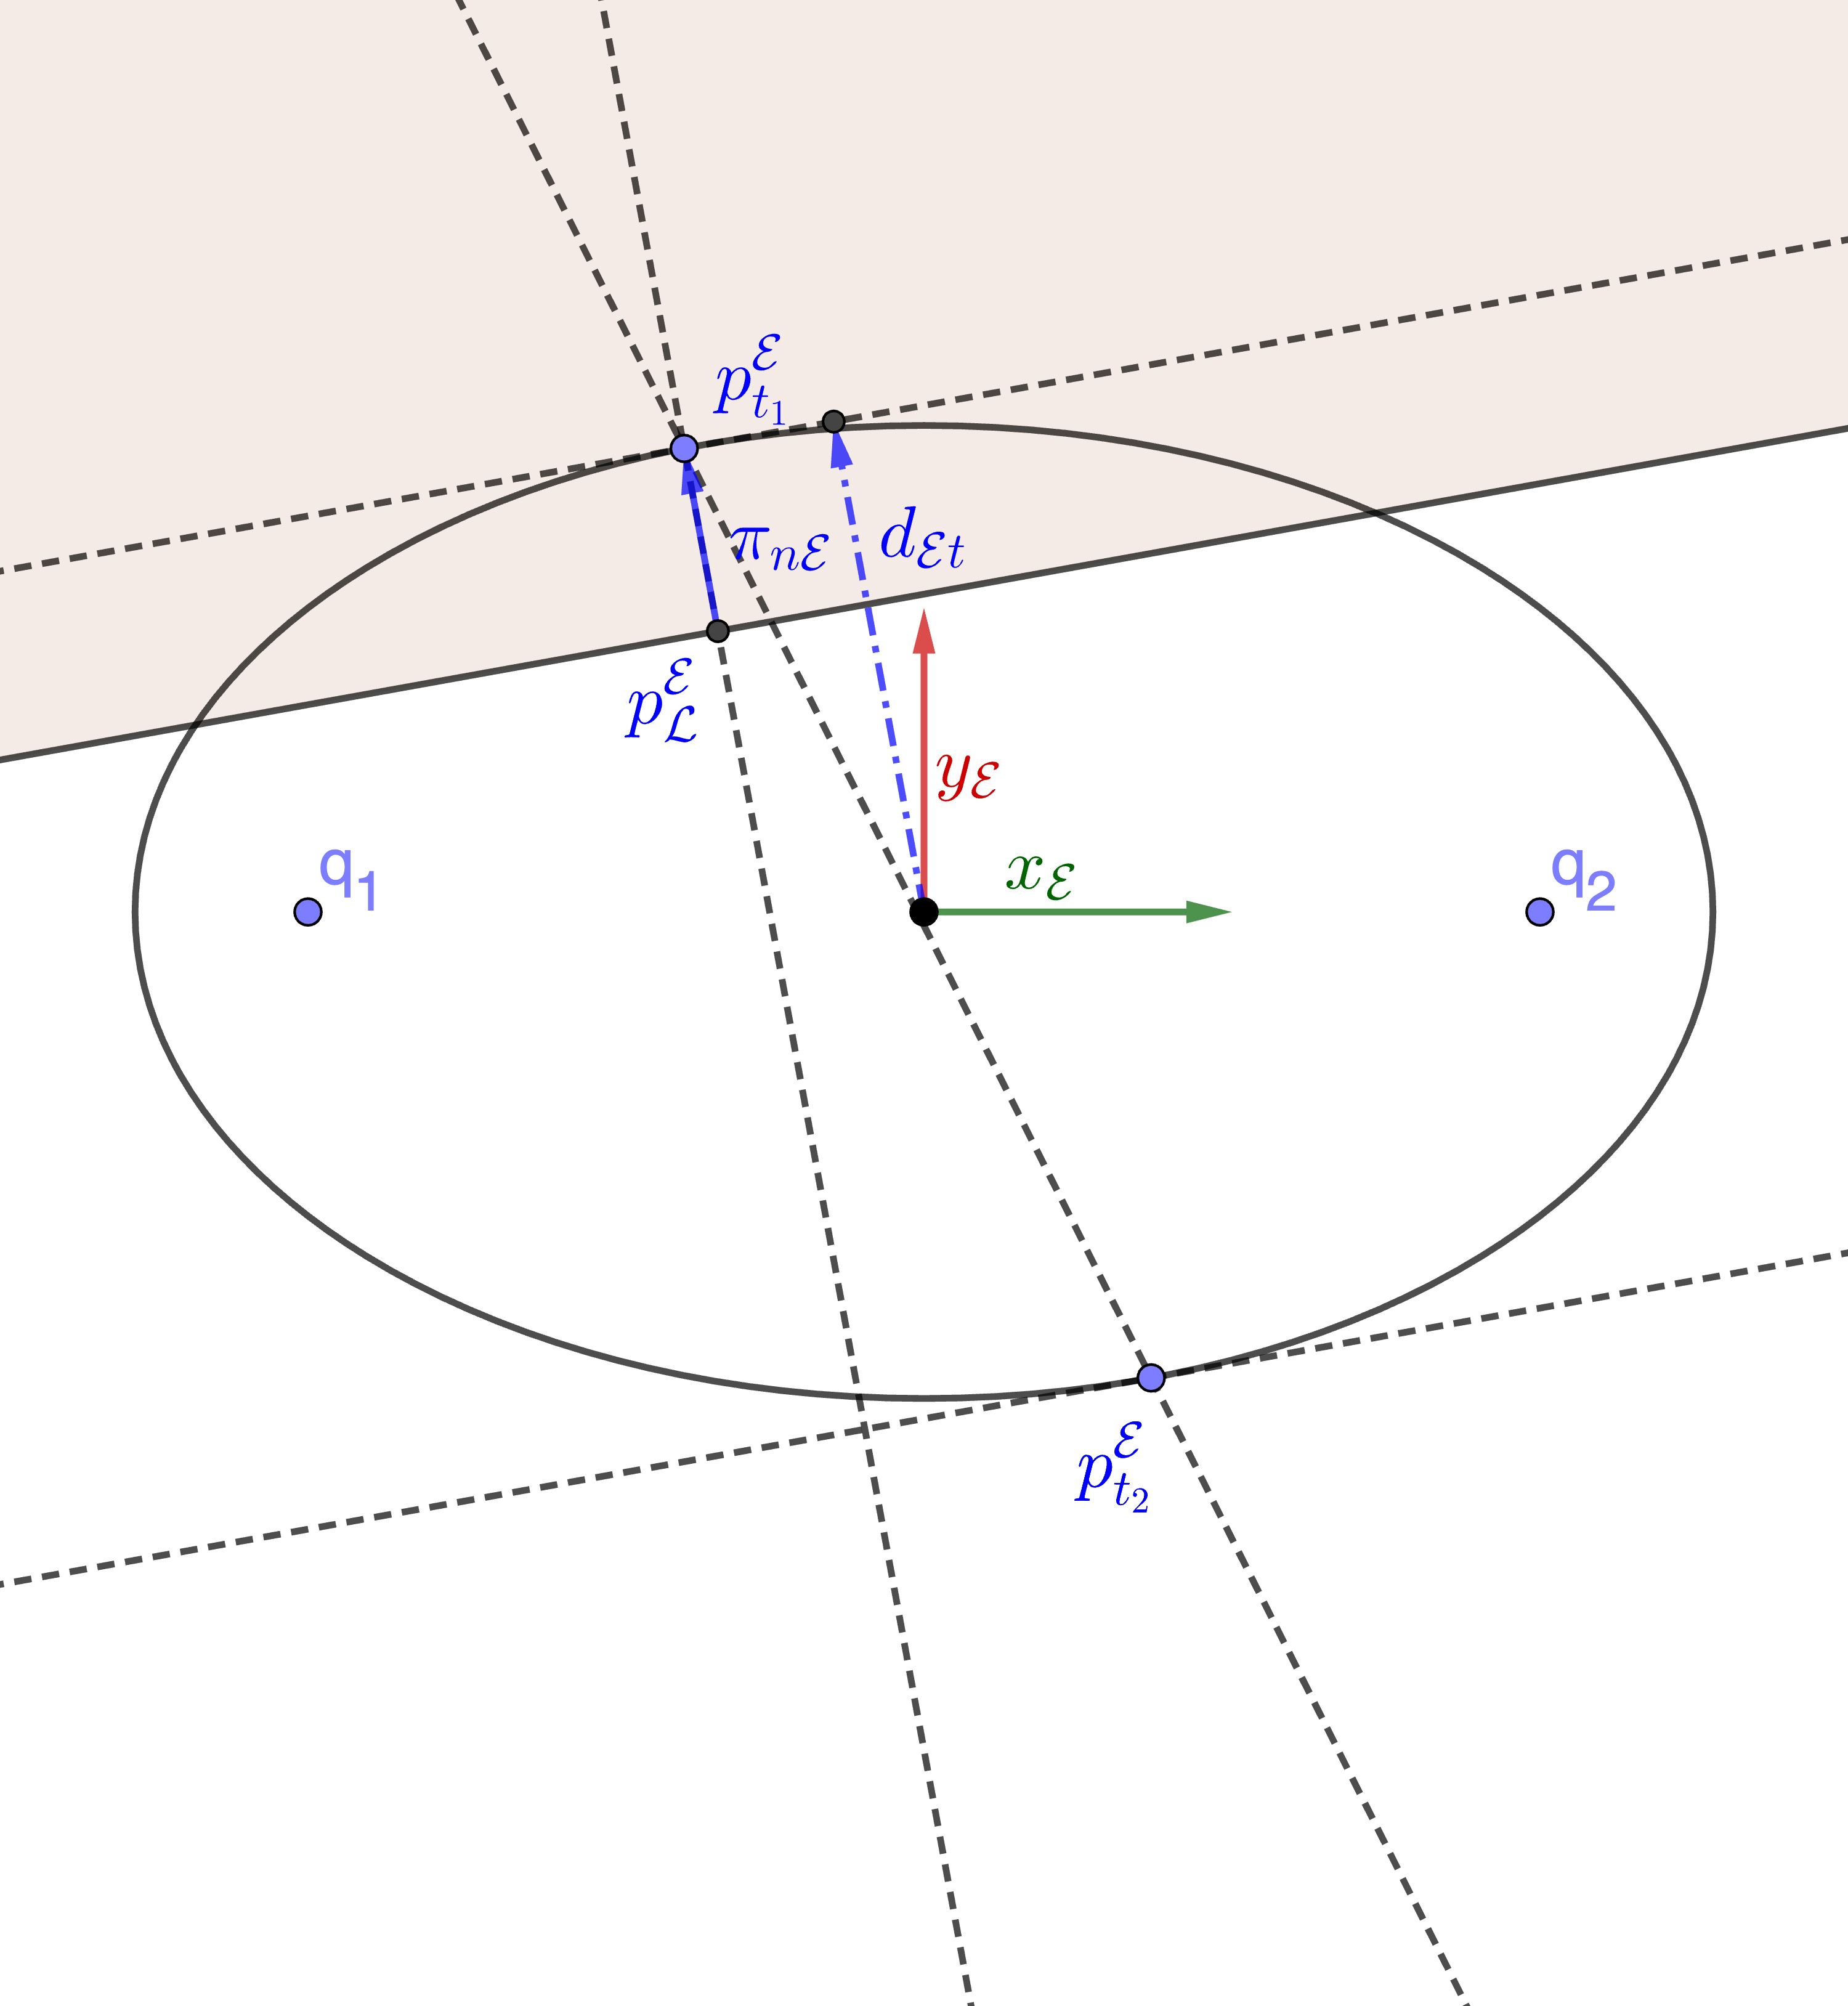
\includegraphics[width=0.47\linewidth, trim = 0.3cm 1cm 0.3cm 1cm, clip]{Ellipse2line_V2}}
    \subfloat[Polygon-ellipse constraint \label{fig:Ellipse-to-safezone}]{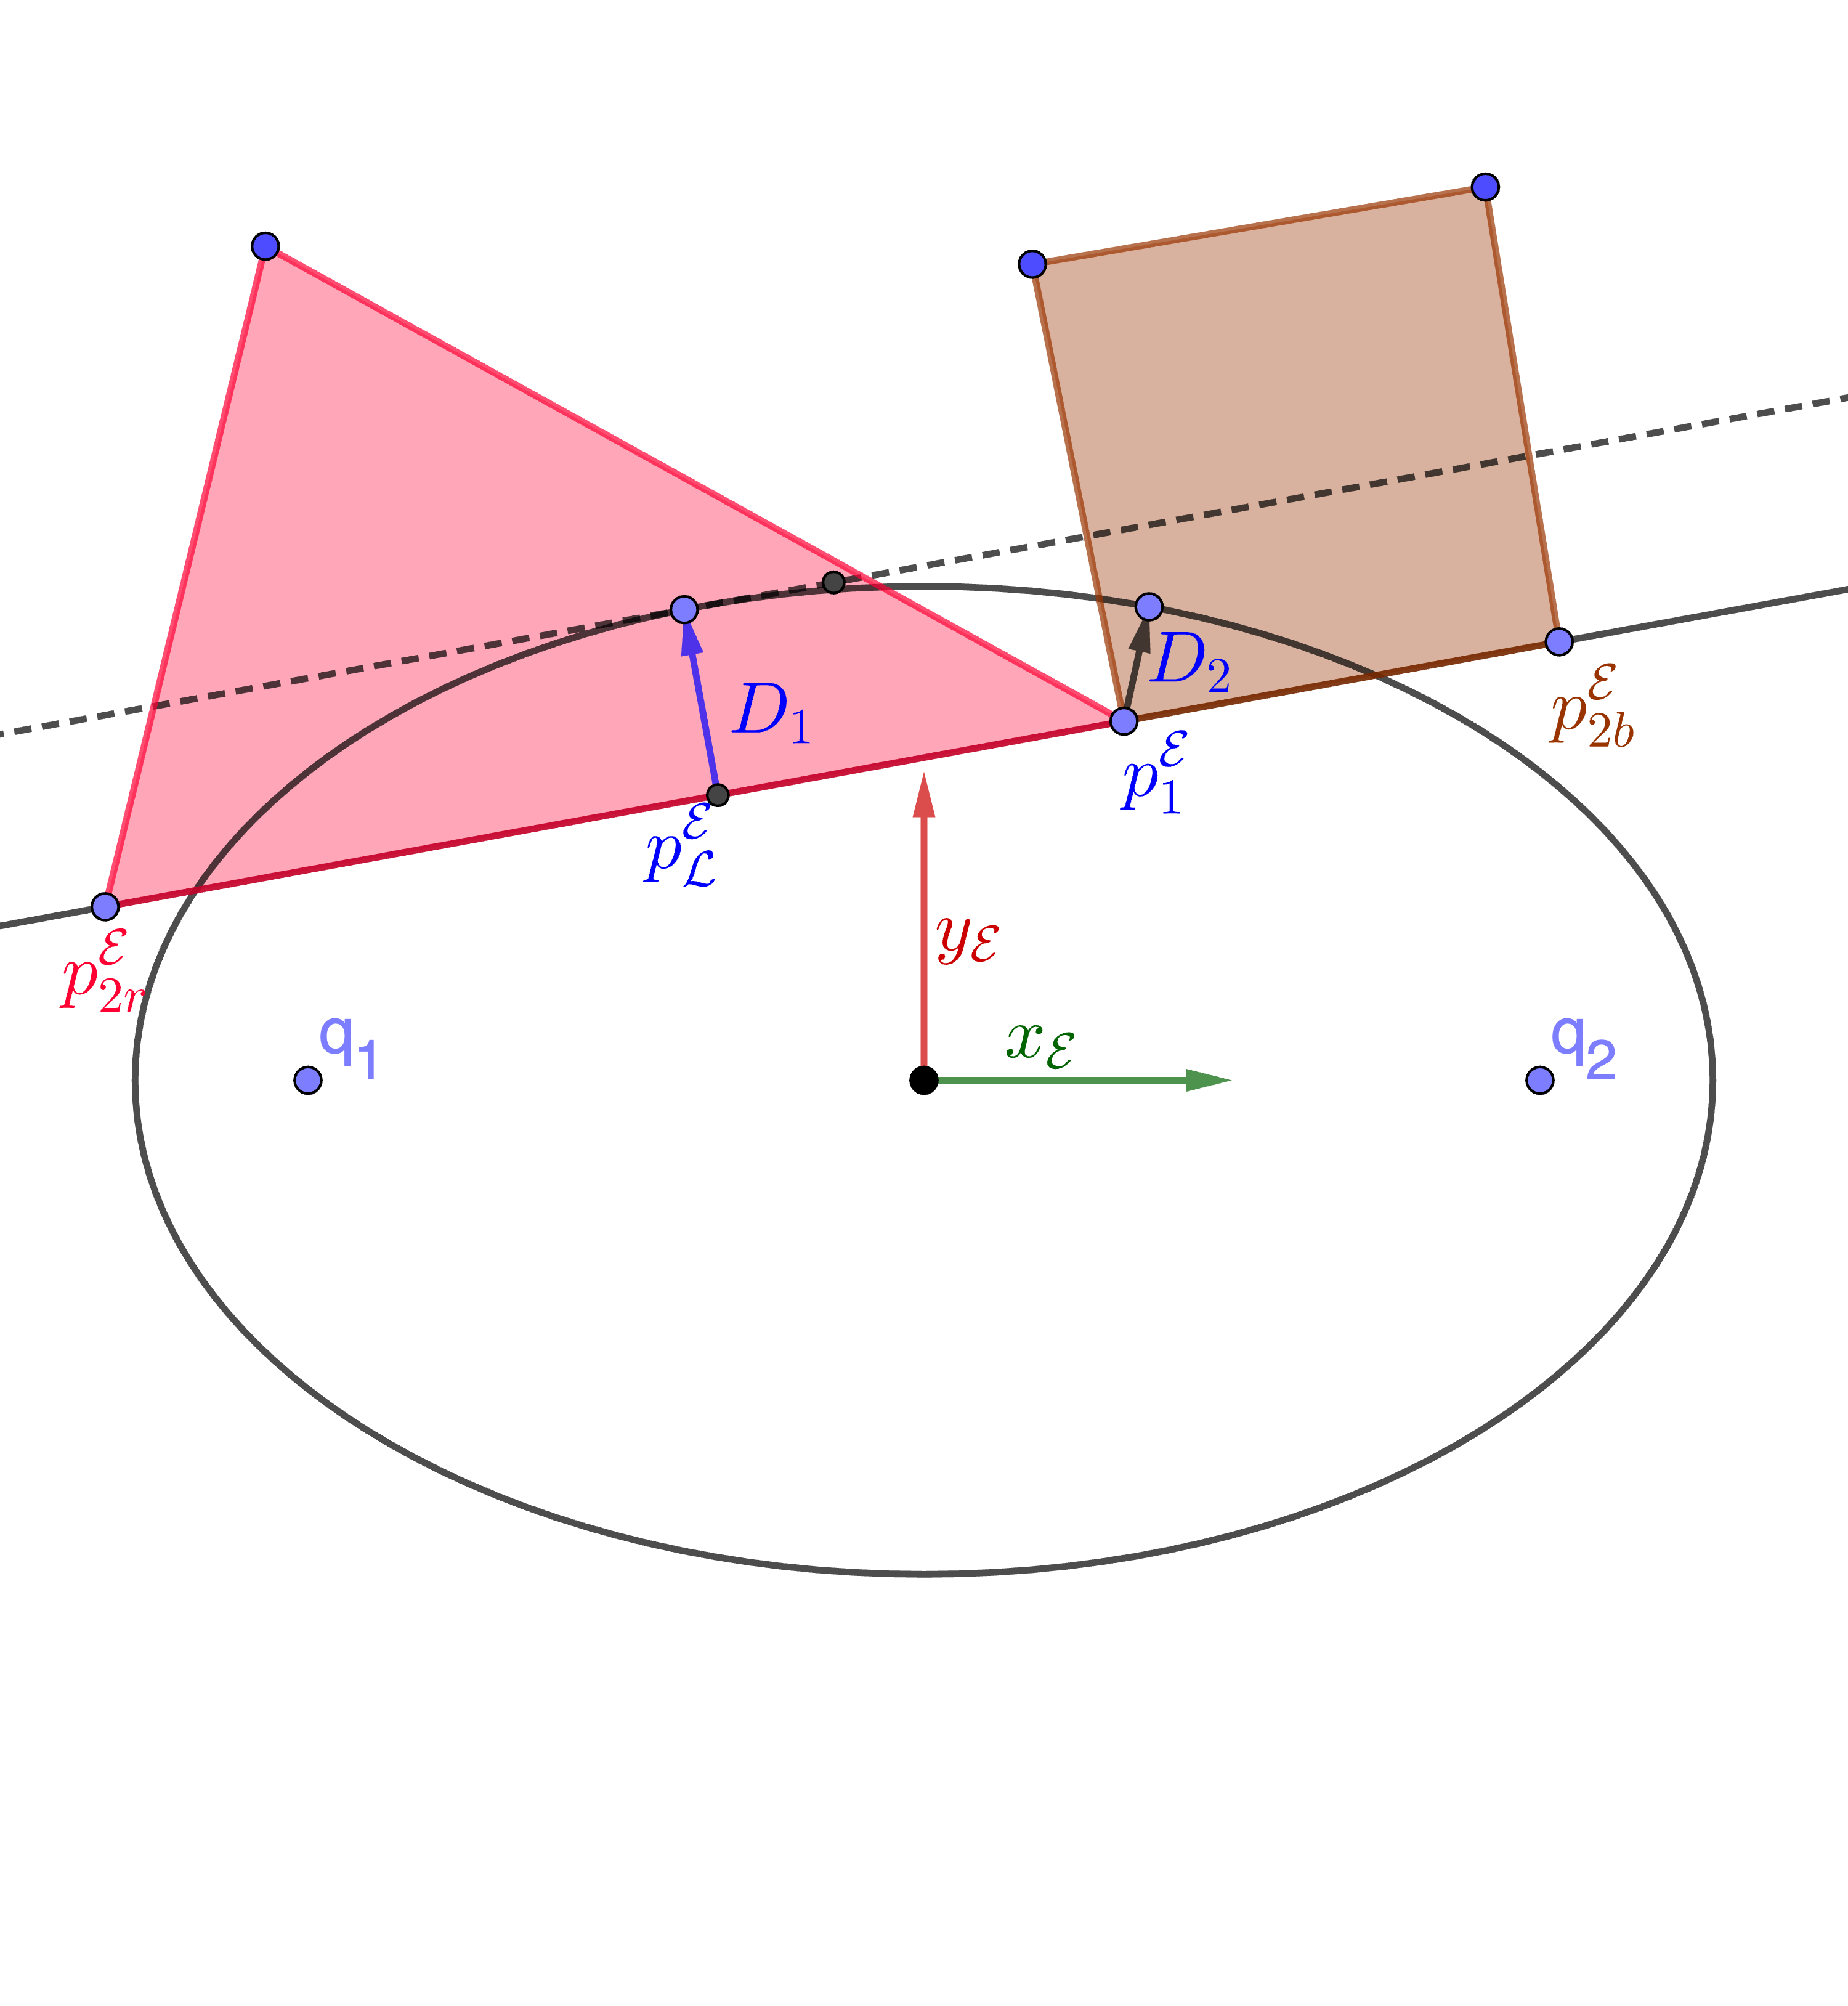
\includegraphics[width=0.47\linewidth,trim = 0cm 1cm 0.3cm 0.5cm, clip]{Ellipse2safezone_V2}}

    \caption{ \Cref{fig:EllipseConstraintExample} showcases the ellipsodial reachability region. Black line is the planned trajectory, $q_1$ and $q_2$ are two co-observed locations the robot are expected at given time $t_1$ and $t_2$, dashed lines show possible trajectory of a compromised robot during unobserved period. Axis of global frame $\cF$ and canonical frame $\cF_{\cE}$ are shown as $x_{\cF}, y_{\cF}$ and $x_{\cE}, y_{\cE}$ respectively. 
    In \Cref{fig:Ellipse-to-point}, a point $q_{avoid}$ inside ellipsoid is projected to the areas outside the ellipsoid $f_{p}$. 
    In \Cref{fig:Ellipse-to-plane}, the projection is simplified to the point-ellipse constraint as projecting a point inside ellipse $p_{L}$ to $p_{t}$ on outside the ellipse.
    In \Cref{fig:Ellipse-to-safezone}, this constraint is simplified to either a plane-ellipse constraint $D_{1}$ or a point-ellipse constraint $D_{2}$.}
    \label{fig:Reachability_full}
  \end{figure}

The region $\cE(q_1,q_2)$ is an ellipsoid with foci at $q_1,q_2$, center $o_{\cE} = \frac{1}{2}(q_1+q_2)$, and the major radius equal to $a$. We denote as $c_\cE=\frac{1}{2}\norm{q_1-q_2}=\norm{o_\cE-q_1}$ the semi-axis distance from the center to a foci. This reachability ellipsoid is an over-approximation of the exact reachability region in \Cref{sec:ellipsoidal definition} \rtron{because the ellipsoid does not consider obstacles}.

Expanding upon the concept of \emph{co-observation} and \emph{reachability}, \Cref{def:secured-plan} can be written as,
\begin{remark}\label{rmk:revised-security}
  A multi-robot trajectory is secured against plan-deviation attacks if there exist a co-observation plan such that the reachability region between each consecutive co-observation does not intersect with any forbidden regions.
\end{remark}

\subsection{Transformation to canonical coordinates}\label{sec:rotation2Standard}
To simplify the problem, we employ a canonical rigid body transformation that repositions the ellipse $\cE$ from the global frame $\cF$ to a canonical frame $\cF_\cE$, and perform this transformation in a differentiable manner with respect to the two foci serving as waypoints for a robot. The canonical frame $\cF_\cE$ is defined with the origin at the ellipsoid's center, and the first axis aligned with the foci \Cref{fig:EllipseConstraintExample}. 

For all reachability ellipsoid constraints, we first solve the problem in the canonical frame $\cF_{\cE}$, and transform the solutions to the global frame $\cF$ using the transformation \eqref{eq:transformations}. We parametrize the transformation from $\cF$ to $\cF_\cE$ using a rotation $R^\cF_\cE$ and a translation $o^\cF_\cE$, which, to simplify the notation, we refer to as $R$ and $o$, respectively. The transformation of a point from the frame $\cF_\cE$ to the frame $\cF$ and its inverse are given by the rigid body transformations:
  \begin{equation}\label{eq:transformations}
    \Fframe{q}=R\Eframe{q}+o,\quad
    \Eframe{q}=R\transpose(\Fframe{q}-o).
  \end{equation}
 
  We define $\nu_\cF$ and $\nu_\cE$ to represent the $x$-axis unitary vector of $\cF_\cE$ in the frames $\cF$ and $\cF_\cE$, respectively. Formally:
  \begin{align}
    \nu'_\cF&=q_2-q_1, & \nu_\cF &= \frac{\nu'_\cF}{\norm{\nu_\cF}}, & \nu_\cE&=[1,0,0]^T;
  \end{align}
  see Fig.\ref{fig:EllipseConstraintExample} for an illustration. Note that $\nu_\cE$ is constant while, for the sake of clarity, $\nu_{\cF}$ depends on $q_1,q_2$. From the definition of $\cF_\cE$, the rotation $R$ can be found using a \emph{Householder rotation}, while from \eqref{eq:transformations} the translation $o$ must be equal to the center of $\cE(q_1,q_2)$ expressed in $\cF$, i.e.:
  \begin{align} 
    R&=H(\nu_\cF(q_1,q_2),\nu_\cE(q_1,q_2)), &o&=\frac{1}{2}(q_1+q_2).
  \end{align}
  To simplify the notation, in the following, we will consider $H$ to be a function of $q_1,q_2$ directly, i.e. $H(q_1,q_2)$. 
  The ellipse $\cE$ expressed in $\cF_\cE$ is given by $\Eframe{\cE}=\{\Eframe{q}\in\real{m}:d(q^\cE_1,\Eframe{q})+d(\Eframe{q},q^\cE_2)<2a\}$, with foci $q^\cE_1,q^\cE_2$ in $\cF_\cE$ defined as
  \begin{align}
    q^\cE_1=\bmat{c & 0 & 0}\transpose, && q^\cE_2=\bmat{-c & 0 & 0}\transpose,
  \end{align}
  and semi-axis distance $c=\frac{\norm{q_2-q_1}}{2}$.
\begin{definition}
  The \emph{reachability ellipsoid $\cE$ in the canonical frame} is defined as as the zero level set of the quadratic function
  \begin{equation}\label{equ:standard-ellipse}
    \Eframe{E}(\Eframe{q}) = \Eframe{q}\transpose Q \Eframe{q} - 1
  \end{equation}
  where
  \begin{equation}
    Q = \diag(a^{-2},b^{-2},b^{-2}),
  \end{equation}
  and $b = \sqrt{a^2-c^2}$.
  The ellipse parameters $a$, $b$ represent the lengths of the major axes.
\end{definition}
\begin{lemma}
The original ellipse $\cE$ in $\cF$ can be expressed as the zero level set of the quadratic function
   \begin{equation}\label{eq:ellpsoid from canonical}
     \Fframe{E}(\Fframe{q}) = (\Fframe{q}-o_\cE)\transpose H\transpose Q H (\Fframe{q}-o_\cE) - 1
     \end{equation}
\end{lemma}
\begin{proof}
    The claim follows by substituting  \eqref{eq:transformations} into \eqref{equ:standard-ellipse}, and from the definition of $R$ and $o$.
\end{proof}

We are now ready to formulate constraints based on reachability ellipsoids against different types of forbidden regions: a point, a plane, a segment, and a convex polygon which is is done by defining $D(q)$, its differential $\partial_qD(q)$, the set $\zeta$ and the projection $\Pi_\zeta$.

\subsection{Point-ellipsoid reachability constraint}\label{sec:ellipsoid-point}
As shown in Fig.\ref{fig:Ellipse-to-point}, we consider a forbidden region in the shape of a single point $q_{avoid}$. The goal is to design the trajectory $q(t)$ such that $q_{avoid}\notin\mathcal{E}(q_1,q_2)$. This constraint can be written as, 

\begin{constraint}[Point-ellipsoid reachability constraint]
\begin{align}
D(\vq) &=  \begin{cases}
      \pi_{p\cE}(\vq) - q_{avoid} & q_{avoid} \in \cE, \\
      {0} & \textrm{otherwise}.
    \end{cases} \label{eq:point_ellipsoid_constraint}\\
  \sZ &= \{q\in\mathbb{R}^{nm}:\norm{D_p(\vq)} = 0 \},\\
   \Pi_\sZ(\vz) & = 0, 
\end{align}
\end{constraint}

where $\pi_{p\cE}(q_{avoid};q_1,q_2,a) = q_p$ is a projection function that returns a projected point $q_p$ of $q_{avoid}$ outside the ellipse, i.e., as the solution to
\begin{equation}\label{eq:ellipse-point-projection}
\pi_{p\cE}=\argmin_{q_p\in\cE^c} \quad \norm{q_{avoid}-q_p}^2 
\end{equation}
where $\cE^{c}$ is the set complement of region $\cE$.

For cases where $q_{avoid} \notin \cE(q(t_2),q(t_1),r)$, $\pi_{p\cE}(q_{avoid}) = q_{avoid}$. And for cases where $q_{avoid} \in \cE(q_1,q_2,r)$, $D(q)$ needs to be projected to the boundary of the ellipse. 
In the canonical frame $\cF_{\cE}$, the projected point $q^{\cE}_{p}$ can be written as:
  \begin{equation}
  	q^\cE_{p} = {(I+sQ)}\inverse q^\cE_{avoid} = S q^\cE_{avoid}
  \end{equation}
  %where $S=(I+sQ)\inverse$.Using the fact that since $q^\cE_p$ is a point on the ellipse, 
where $s$ can be solved as the root of the level set \eqref{equ:standard-ellipse}:
  \begin{equation}
    {q^\cE_p}\transpose Q q^\cE_p-1={q^\cE_{avoid}}\transpose Q'(s) q^\cE_{avoid} -1=0
  \end{equation}
  where
  \begin{equation}
    Q'(s) =S\transpose Q S = \diag\left(\frac{a^{2}}{(s+a^{2})^2}, \frac{b^{2}}{(s+b^{2})^2},\frac{b^{2}}{(s+b^{2})^2}\right)
  \end{equation}
 Detailed methods for computing $s$ can be found in \cite{yang2021multi,yang2020multi,eberly}. 


  %The point to project, $q_{avoid}$, can be likewise expressed in $\cF_\cE$ as $\Eframe{q}_{avoid} =  H (\Fframe q_{avoid}-o)$. We now turn our attention to the problem of projecting $\Eframe{q}_{avoid}$ on the zero level set of $E^\cE$ (i.e., the reachability ellipsoid in the canonical frame). The derivations below are loosely inspired by \cite{eberly}.

  %Let $q^\cE_p$ be the point on the surface of the ellipsoid, i.e., $\Eframe E(q^\cE_p) = 0$, corresponding to the projection of the point $q^\cE_{avoid}$. Using Lagrange multipliers applied to the constrained optimization problem \eqref{eq:ellipse-point-projection} (after transforming it in the canonical frame), one can show that the vector from a point to its projection, $q^\cE_{avoid}- q^\cE_p$, must be collinear with the gradient of $\Eframe \cE$, i.e.
 % \begin{equation}
 %   q^\cE_p- q^\cE_{avoid} = s \partial_q \Eframe E(q^\cE_p)\transpose = s Q q^\cE_p
  %\end{equation}
  %for some scale $s\in\real{}$;
 % thus $q^\cE_p$ can be written as:

The point-to-ellipse projection function in $\cF$ is then:
  \begin{multline}\label{equ:Point2EllipseProjection}
    \pi_{p\cE}(q)= R^{-1}(q(t_1),q(t_2))q^\cE_p+o \\
    = R^{-1}(q(t_1),q(t_2))Sq^\cE_{avoid}+o\\
    = R^{-1}S R ( q_{avoid}- o)+o
  \end{multline}
  
  In our derivations, we consider only the 3-D case ($m=3$); for the 2-D case, let $P=\bmat{I & 0}\in\real{2\times 3}$: then $\pi_{p\cE}^{\textrm{2D}}=P\pi_{p\cE}^{\textrm{3D}}(P\transpose q_{avoid}; P\transpose q_1, P\transpose q_2,a)$.

  \begin{proposition}\label{prop:Ellipse2PointDiff}
    The differential of the projection operator $\pi_{p\cE}(q_{avoid}; q_1,q_2,a)$ with respect to the foci $q_1,q_2$ is given by the following (using $q$ as a shorthand notation for $q^\cE_{avoid}$)
    \begin{multline}
      \partial_{\left[\begin{smallmatrix}q_1\\q_2\end{smallmatrix}\right]} \pi_{p\cE}=-2 H [ SH(q-o)]_{\times}U   \\
      + \left( (q\transpose \partial_sQ' q)^{-1} H^{-1} Q' q q\transpose  (4Q' H[q - o]_\times U \right. \\
      \left.+ 2Q' H\partial_q o - \partial_b Q' q q \partial_q b) -  s H^{-1} S^2 \partial_b Q q \partial_q b\right) \\
      -2H^{-1} S H[q-o]_{\times} U  + (H^{-1}SH -I)\partial_q o
    \end{multline}
  \end{proposition}
  \begin{proof}
  See \Cref{proof:Ellipse2PointDiff}.
  \end{proof}
  The differential of $D_p$ is the same as the one for $\pi_{p\cE}$.

\subsection{Plane-ellipsoid reachability constraint}\label{sec:ellipsoide-plane}

For forbidden region in the shape of a hyperplane $\mathcal{L}(\Fframe{q}) = \{\Fframe{q}\in\mathbb{R}^n: \vn\transpose \Fframe{q} = d\}$ (as shown in Figure \ref{fig:Ellipse-to-plane}), the reachability constraint can be defined as $\mathcal{L} \cap \mathcal{E}(q_1,q_2,a) = \emptyset$. When transformed into the canonical frame, the hyperplane can be written as $\Eframe \cL(\Eframe{q}) = \{  \Eframe{q}\in\mathbb{R}^m:  \vn_\cE\transpose \Eframe{q} = d_{\cE}\}$, where,
  \begin{equation}
    \vn_\cE = H(q_1,q_2)\vn, \quad d_\cE =-\vn\transpose o + d.
\end{equation}
Intuitively, $d_\cE$ can be thought as a distance between the the plane $\cL$ and the origin (i.e., the center of $\cE$).

For every $\Eframe \cL(\Eframe{q})$, there always exist two planes that are both parallel to $\cL$ and tangential to the ellipse (i.e. resulting in a unique intersection point), $\cL_1^{\cE} = \{\Eframe{q}\in\mathbb{R}^m: \vn_\cE \transpose \Eframe{q} =  d_{\cE t} \}$ and $\cL_2^{\cE} = \{\Eframe{q}\in\mathbb{R}^m: \vn_\cE \transpose \Eframe{q} = - d_{\cE t} \}$  (\Cref{fig:Ellipse-to-plane}). And the intersection point can be written as:
\begin{equation}
    p^\cE_{t_{1}} = \frac{ d_{\cE t} Q^{-1}   n_\cE}{ n_\cE \transpose Q^{-1}  n_\cE} = \frac{Q^{-1} n_\cE}{ d_{\cE t}},\quad  p^\cE_{t_{2}} = -  p^\cE_{t_{1}},
\end{equation}
where $d_{\cE t} = \sqrt{ n_\cE\transpose Q^{-1} n_\cE}$; intuitively, $d_{\cE t}$ can be thought as a distance between the tangent plane $\cL_1^\cE$ (or $\cL_2^\cE$) and the origin (i.e., the center of the ellipse $\cE$).

We introduce the concept of a tangent interpolation point on the hyperplane to characterize the relationship between the plane and the ellipse.

\begin{definition}
The \emph{tangent interpolation point} $p^\cE_{\cL} \in \mathcal{L}$ is defined on the plane by 
    \begin{equation}\label{equ:ProjectPoint}
      p^\cE_{\cL} = \frac{ d_\cE Q^{-1} n_\cE}{ n_\cE\transpose Q^{-1} n_\cE}.
    \end{equation}
  Intuitively, the point $p^\cE_\cL$ is the point on $\cL$ which is closest to either $p^\cE_1$ or $p^\cE_2$.
  Note that when  $d_\cE=d_{\cE t}$ or $d_\cE=-d_{\cE t}$, $p^\cE_{\cL}=p^\cE_{t_1}$ or $p^\cE_{\cL}=p^\cE_{t_2}$, respectively. When $ d_\cE \in [- d_{\cE t},  d_{\cE t}]$, the plane $\cL$ and the ellipsoid $\cE$ have at least one intersection, thus violating our desired reachability constraint. 
\end{definition}

With these definitions, the constraint can be written as:

\begin{constraint}[Plane-ellipsoid reachability constraint]
\begin{align}
D(\vq) &= H^{-1}(q_{1},q_2)\pi^\cE_{\vn_\cE}(\vq)+o, \label{eq:plane_ellipsoid_constraint}\\
  \sZ &= \{\vq\in\mathbb{R}^{nm}:\norm{D_{\vn}(\vq)} = 0 \},\\
   \Pi_\sZ(\vz) & = \overrightarrow{0}, 
\end{align}
\end{constraint}
where $\pi^\cE_{\vn_\cE}(q)$ is the projection operator defined as:
  \begin{equation}\label{equ:plane2ellipse}
    \pi^\cE_{\vn_\cE}(\vq) =\begin{cases}
      p^\cE_{t_1}-p^\cE_{\cL} & \textrm{ if } d_\cE \in [0, d_{\cE t}], \\
      p^\cE_{t_2}-p^\cE_{\cL} &  \textrm{ if } d_\cE \in [- d_{\cE t},0), \\
      {0} & \textrm{otherwise}.
    \end{cases}
  \end{equation}

  \begin{proposition}\label{prop:dpi_ne_dt}
    The differential of the projection function $\pi^\cE_{\vn \cE}(\vq)$ with respect to the foci $q_1$ and $q_2$ is given by:
    \begin{equation}
      \partial_q \pi^\cE_{\vn \cE}(q) = \begin{cases}
        \partial_q p^\cE_{t1}-\partial_q p^\cE_{\cL} &  d_\cE \in [0, d_{\cE t}], \\
        \partial_q p^\cE_{t2}-\partial_q p^\cE_{\cL} &  d \in [- d_{\cE t},0), \\
        {0} & otherwise.
      \end{cases}
    \end{equation}
    where
    \begin{multline}
      \partial_q p_\cL =   (-\frac{d_{\cE t} n\transpose \partial_q o -2d_\cE \partial_q d_{\cE t}}{d_{\cE t}^3} )Q^{-1}n_\cE \\
      + \frac{d_\cE\partial_b Q^{-1} n_\cE \partial_q b -  2d_\cE Q^{-1}H[n]_\times U}{d_{\cE t}^2},
    \end{multline}
    \begin{equation}
      \partial_q p_{1} =  -\frac{Q^{-1}n_\cE \partial_q d_{\cE t} }{d_{\cE t}^2} 
      + \frac{\partial_b Q^{-1}n_\cE \partial_q b -  2Q^{-1}H[n]_\times U }{d_{\cE t}}.
    \end{equation}
  \end{proposition}
  \begin{proof}
  See \Cref{proof:dpi_ne_dt}.
  \end{proof}
  Based on the \Cref{prop:dpi_ne_dt}, the differential of (\ref{eq:plane_ellipsoid_constraint}) can be written as:
  \begin{equation}
    \partial_q {D_{\vn\cE}} = -2 H \cross{\Eframe \Pi_{\vn \cE}}  M + H^{-1}\partial_q \Eframe \Pi_{\vn \cE}
  \end{equation}

\subsection{Line-segment-ellipse reachability constraint}\label{chapter:ellipse to segment}

For a intermediate step to get the relationship between a polygon shaped forbidden region, the relative position between the ellipse and segment of the hyperplane that defines the region is studied. 
Assume the segment on hyperplane $\Eframe \cL(\Eframe q) = \{ \Eframe q\in\mathbb{R}^m:  \vn_\cE\transpose \Eframe q = d_{\cE}\}$ has endpoints $\Eframe {p_1}$ and $\Eframe{p_2}$; then the segment can be defined as:
\begin{equation}
\bmat{(\Eframe {p_1}- \Eframe{p_2})\transpose\\( \Eframe{p_2} - \Eframe{p_1})\transpose}  \Eframe p \leq \bmat{ \Eframe{p_2}\transpose\\- \Eframe{p_1}\transpose}( \Eframe{p_1}- \Eframe{p_2}), \quad \vn_\cE\transpose \Eframe q = d_{\cE}.
\end{equation}
For cases, where the \emph{tangent interpolation point} $\Eframe{p_{\cL}}$ stays within the segment (i.e. red region in \Cref{fig:Ellipse-to-safezone}, where $\Eframe{p_{\cL}}$ lies between $\Eframe{p_{1}}$ and $\Eframe{p_{2r}}$), the constraint can be seen as a plane-ellipse constraint in \Cref{sec:ellipsoide-plane}. Otherwise (i.e. brown region in \Cref{fig:Ellipse-to-safezone}, where $\Eframe{p_{\cL}}$ lies outside $\Eframe{p_{1}}$ and $\Eframe{p_{2b}}$), the constraint can be seen as a point-ellipse constraint in \Cref{sec:ellipsoid-point}.

\begin{constraint}[Line-segment-ellipsoid reachability constraint]
\begin{align}
D(\vq) &=  \begin{cases}
D_{p_{1}}(\vq) & (\Eframe{p_1}-\Eframe{p_2})\transpose (\Eframe{p_{\cL}}-\Eframe{p_2})<0\\
D_{p_{2}}(\vq) & (\Eframe{p_2}-\Eframe{p_1})\transpose (\Eframe{p_{\cL}} -\Eframe{p_1})<0\\
D_\Eframe{p_{\cL}}(\vq) & \textrm{otherwise}
\end{cases} \label{eq:segment_ellipsoid_constraint}\\
  \sZ &= \{\vq\in\mathbb{R}^{nm}:\norm{D(\vq)} = 0 \},\\
   \Pi_\sZ(\vz) & = 0, 
\end{align}
\end{constraint}
where $D_{p_{1}}$ and $D_{p_{2}}$ are the point-ellipsoid constraint projection function with respect to $\Eframe{p_{1}}$ and $\Eframe{p_{2}}$ in \eqref{eq:point_ellipsoid_constraint}, and $D_\Eframe{p_{\cL}}$ is the plane-ellipsoid constraint with respect to frame $\Eframe {\cL}$ in \eqref{eq:plane_ellipsoid_constraint}.


\subsection{Convex-polygon-ellipse reachability constraint}\label{sec:ellipse-region-constraint} 
To keep an ellipse away from a convex polygon, first, we need to keep all segments of the hyperplanes outside the ellipse. Similar to \eqref{equ:ProjectPoint}, we define
\begin{constraint}[Convex-polygon-ellipsoid reachability constraint]\label{constraint:polygon-ellipsoid}
\begin{align}
D(\vq) &= \bmat{D_{seg1}(\vq)\\D_{seg2}(\vq)\\ \vdots} \label{eq:region_ellipsoid_constraint}\\
  \sZ &= \{\vq\in\mathbb{R}^{nm}:\norm{D(\vq)} = 0 \},\\
   \Pi_\sZ(\vz) & = 0, 
\end{align}
\end{constraint}
where $D_{seg}$ are the constraint functions for each line segment used to define convex polygon region. ADMM constraint~\ref{constraint:polygon-ellipsoid} needs to be supplemented with a convex obstacle constraint for the polygon (as introduced in \cite{yang2020multi}) to prevent cases where the ellipse is a subset of the region.

\subsection{Secured planning results and limitation}\label{sec:ADMM-simulation}

In this section, we apply the newly introduced security constraints to a map exploration problem, illustrated in \Cref{fig:example-application}. The algorithm is tested in both simulations and on an experimental testbed, involving a 3-robot system assigned to explore a $10m\times10m$ region with one obstacle, \emph{Zone 1}, and two forbidden zones, \emph{Zone 2} and \emph{Zone 3}. The maximum velocity constraint $v_{max}=0.5m/dt$, time horizon $T=20$. All robots are tasked with collecting sensor information on the vector field, with higher accuracy of sensor data for locations closer to the agent. %robots are expected to follow a boustrophedon pattern (similar to the unconstrained result in Figure~\ref{fig:SecurityBreak}). %We apply the new security constraints on the map exploration problem shown in \Cref{fig:example-application}, test the algorithm in both simulations and an experimental testbed. The 3-robot system is tasked to explore a $10m\times10m$ region with two forbidden regions \emph{Zone 2, 3}. The maximum velocity constraint $v_{max}$ is set to~$0.5m/dt$ a time limit of 20. 

We employ the APMAPF solver from \cite{wardega2019resilience} to generate a MAPF plan with a co-observation schedule in a grid-world application (Fig.\ref{fig:Grid-example-application}). Agents 1 and 2 need to meet at times 8 and 14, while agents 2 and 3 need to meet at time 18. This result serves as the initial trajectory input for the ADMM solver. This obtained plan is then transformed to a continuous configuration space, addressing map exploration tasks. Co-observation schedules are set up using the APMAPF algorithm for two forbidden regions. Reachability constraints are added to ensure an empty intersection between all robots' reachability regions during co-observations and the forbidden regions. It's important to note that the secured attack-proof solution is initially infeasible in the continues setting, unless additional checkpoints (e.g., stationary security cameras) are incorporated (additional task added for agent 3 to visit the \emph{checkpoint} at time $8$). Further solutions to avoid these checkpoints are discussed in \Cref{sec:cross-trajectory}.

The simulation result, shown in Fig.~\ref{fig:ReachabilitySimulation}, displays reachability regions as black ellipsoids, demonstrating empty intersections with Zones 2 and 3. Explicit constraints between reachability regions and obstacles are not activated, assuming basic obstacle avoidance capabilities in robots. The intersections between obstacles and ellipsoids, as observed between agent 3 and Zone 1, are deemed tolerable. All constraints are satisfied, and agents have effectively spread across the map for optimal exploration tasks.


%As depicted in Fig.\ref{fig:Grid-example-application}, no explicit tasks are assigned besides the start and goal locations. Agents 1 and 2 need to meet at times 8 and 14, while agents 2 and 3 need to meet at time 18. This result serves as the initial trajectory input for the ADMM solver. Considering this schedule, reachability for all agents in-between scheduled co-observations is constrained and kept away from the forbidden regions. % It's important to note that additional checkpoints (e.g., stationary security cameras) need to be incorporated to generate an attack-proof solution. Further solutions to avoid these checkpoints are discussed in \Cref{sec:cross-trajectory}.

%We utilize the APMAPF solver introduced in \cite{wardega2019resilience} to generate a MAPF plan with co-observation schedule on a grid-world application (Fig.\ref{fig:Grid-example-application}) and transform the result to a continuous configuration space, under the map exploration tasks.  All robots have the task of collecting sensor information on the underlying vector field, with agent 3 having an additional task to visit the \emph{checkpoint} at time $8$. Assuming that the sensors on the robots return data with higher accuracy for locations closer to the agent, the robots should ideally perform a boustrophedon pattern (like the unconstraint result in Figure~\ref{fig:SecurityBreak}). We first set up an co-observation schedules considering two forbidden regions using the APMAPF algorithm, and add reachability constraints ensure a empty intersection between all robots' reachability regions between co-observations and forbidden regions.

%As shown in Fig.\ref{fig:Grid-example-application}, no task has been assigned to the agent besides the start and goal location. Agent 1 and 2 need to meet at time 8 and 14, whereas agent 2 and 3 need to meet at time 18. This result is also used as the initial trajectory input for the ADMM solver. 

%Based on the schedule, reachability for agent 1 in-between the scheduled co-observations are constrained. Notice that additional checkpoint (i.e. stationary security camera) need to be incorporated in order to generated an attack-proof solution. Additional solutions to avoid these checkpoints will be discussed in \Cref{sec:cross-trajectory}.  
%The result of the simulation is shown in Fig.~\ref{fig:ReachabilitySimulation}. The reachability regions are shown as black ellipsoids, and we can show that all of them have empty intersections with Zone 2 and 3. Notice that no explicit constraints have been enabled between reachability regions and obstacles, because we assume that robots have the basic obstacle avoidance capability and can not go through any hard obstacles. Therefore, the intersections between obstacles and ellipsoids, i.e. the case here between agent 3 and zone 1, are tolerable. All constraints have been satisfied and, to the best of their capability, agents have spread out across the map to perform the best possible exploration task. 

\begin{figure}
\begin{center}
  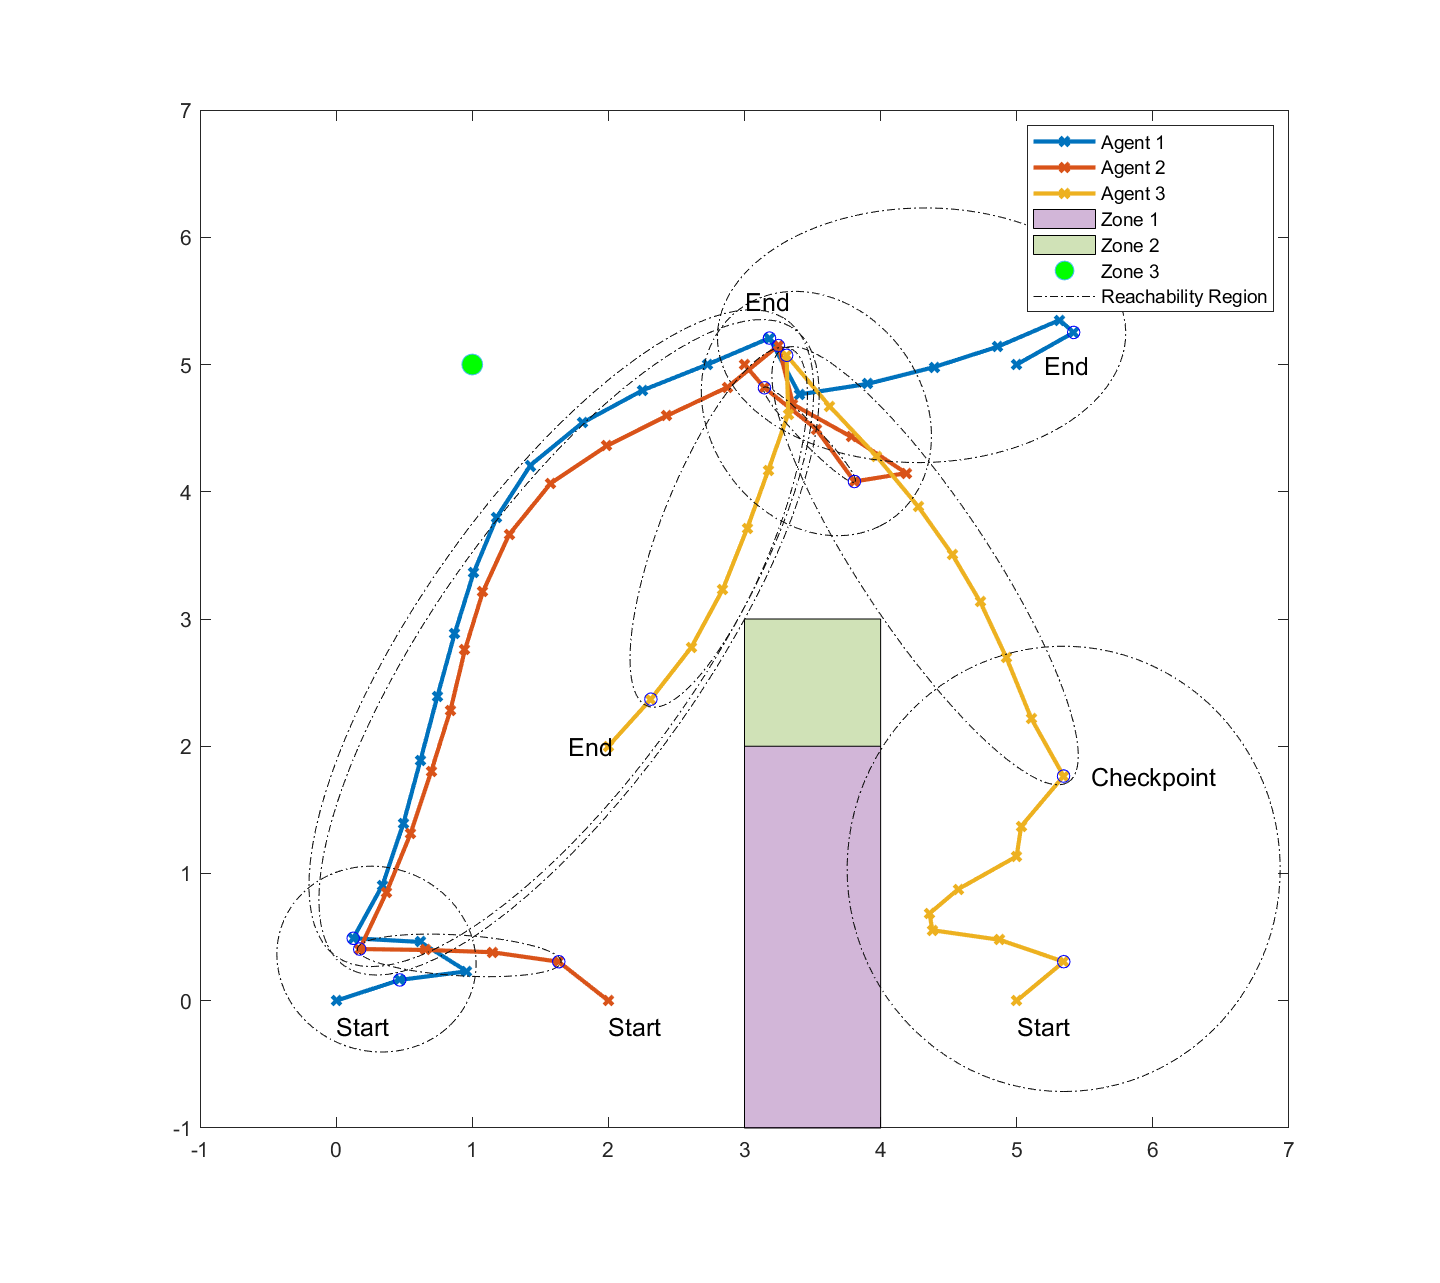
\includegraphics[width=0.6\linewidth,trim =1cm 1.5cm 1cm 1.5cm, clip]{FinalResult}
  \caption{Securd result using co-observation and reachability constraints.}
\label{fig:ReachabilitySimulation}
\end{center}  
\end{figure}

% \begin{figure}[htbp]
% \centering
% %\subfloat[Unsecured optimal trajectory\label{fig:SecurityBreak}]{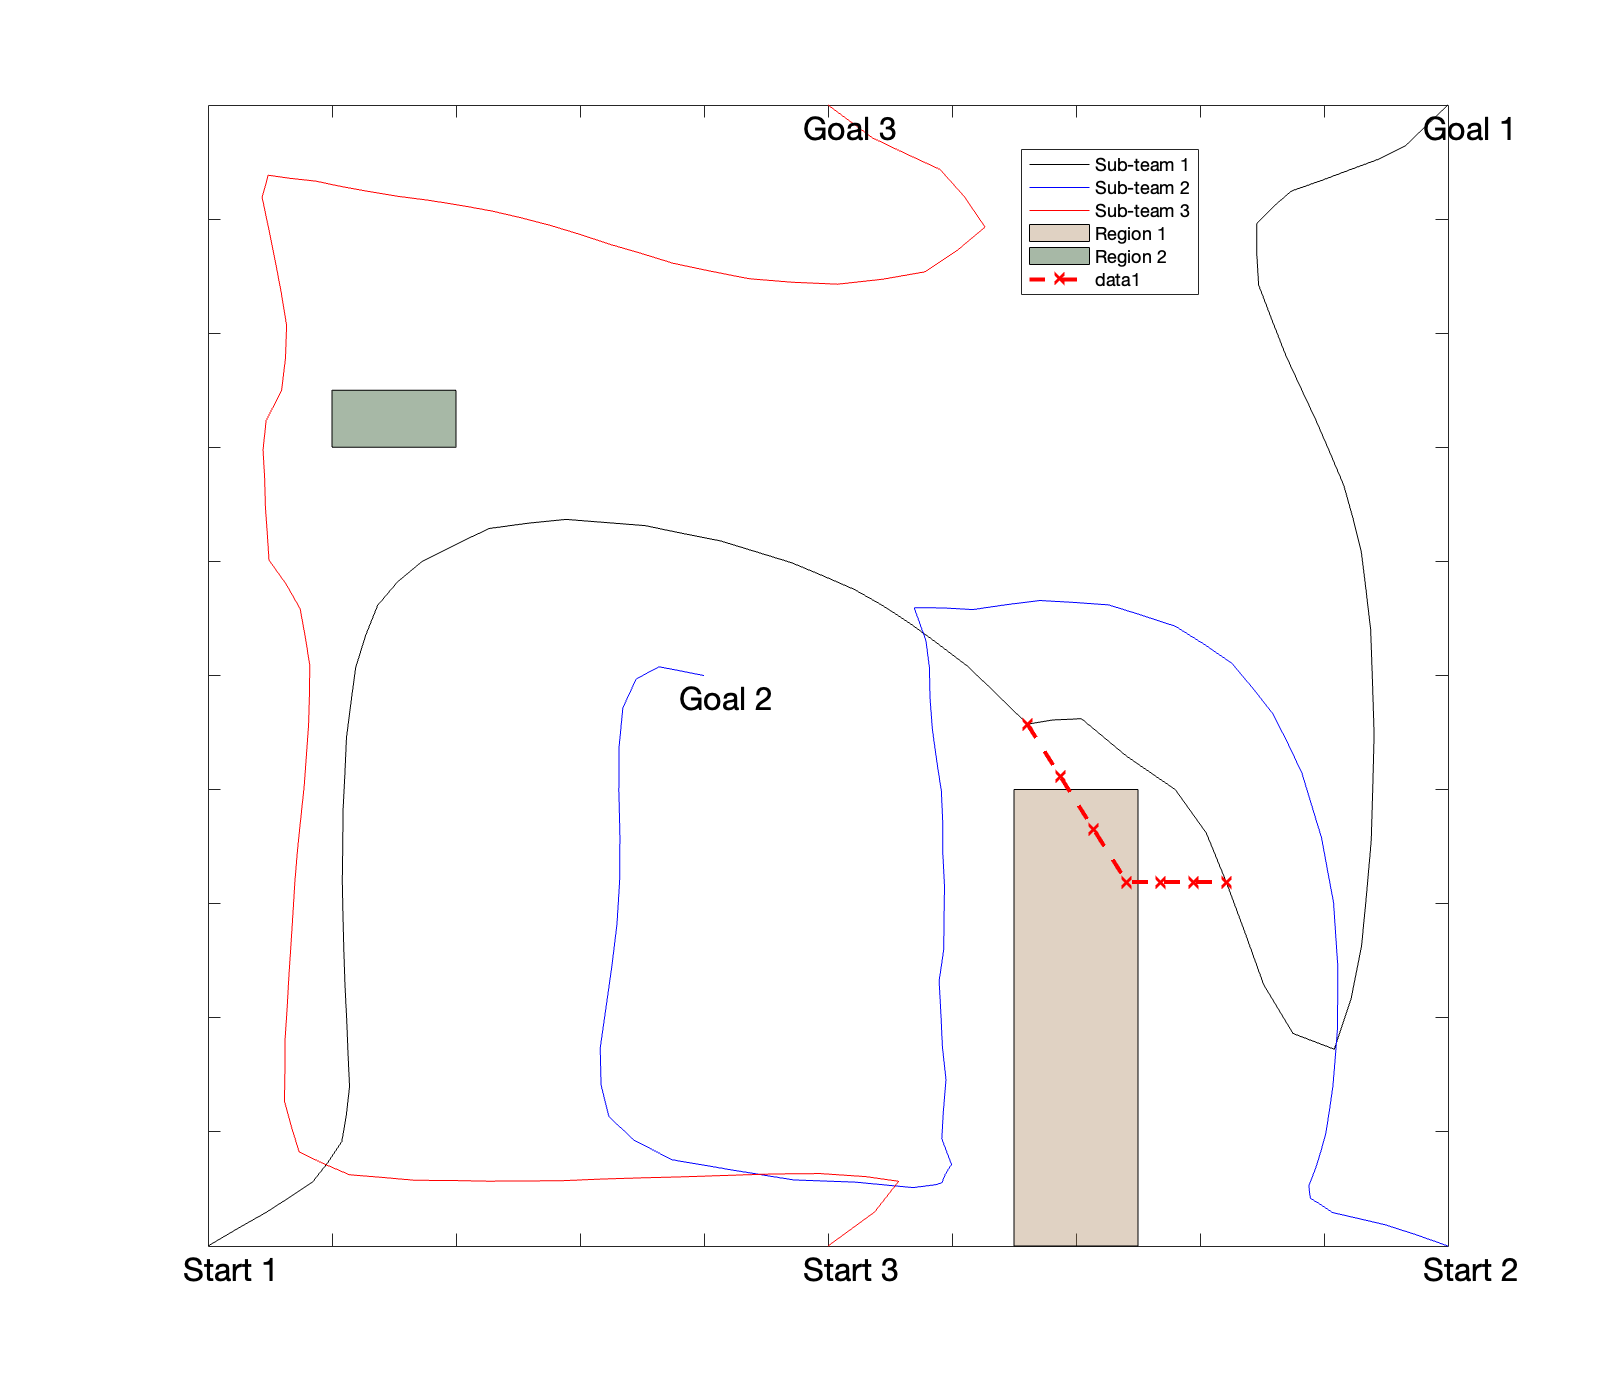
\includegraphics[width=0.47\linewidth, trim =1cm 2cm 1cm 2cm, clip]{SecurityBreak}}
% \subfloat[Secured trajectory\label{fig:ReachabilitySimulation}]{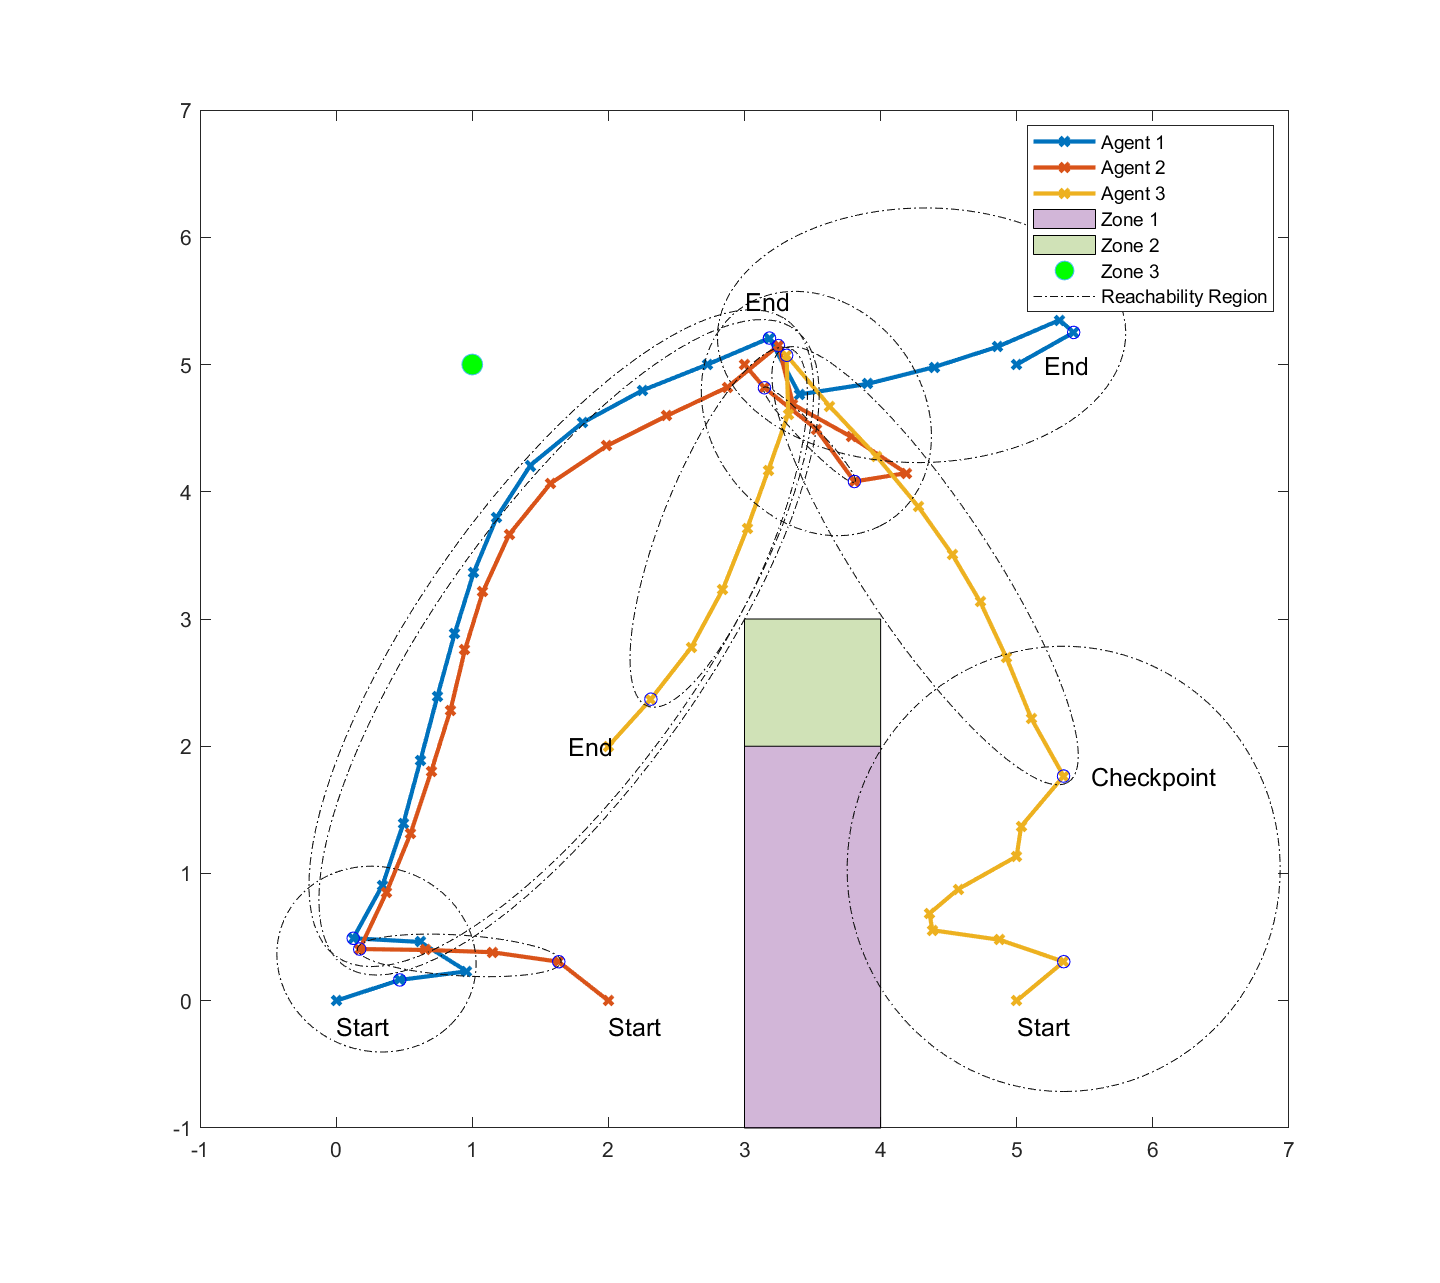
\includegraphics[width=0.6\linewidth]{FinalResult}}

% \caption{ is the securd result with co-observation and reachability constraints.}
% \label{fig:2_ADMM_result}
% \end{figure}

\subsubsection{Limitations}\label{sec:reachability-discussion}
Our solution demonstrates the potential of planning with reachability and co-observation to enhance the security of multi-agent systems. However, two primary challenges need to be addressed. Firstly, achieving a co-observation and reachability-secured plan may not always be feasible when robots are separated by obstacles or forbidden regions, making it impossible for them to establish co-observation schedules or find a reachability-secured path. For example, Agent 3 in Figure \ref{fig:ReachabilitySimulation} required an additional security checkpoint to create secured reachability areas. Secondly, meeting security requirements may impact overall system performance, as illustrated by the comparison between Figure \ref{fig:SecurityBreak} and \ref{fig:ReachabilitySimulation}. The introduction of security constraints led to the top left corner being unexplored by any robots. This trade-off between security and system performance is particularly significant given that system performance plays a crucial role in the decision to employ multi-agent systems. These challenges are addressed in Chapter \ref{sec:cross-trajectory} to ensure the effective use of planning with reachability and co-observation in securing multi-agent systems.

%Our solution shows that planning with reachability and co-observation is a promising approach to enhance the security of multi-agent systems. However, two main challenges have been identified in \cite{wardega2023hola}. Firstly, finding a co-observation and reachability secured plan may not always be feasible when robots are separated from others by obstacles or forbidden regions, or are located far away from each other. In such case, it is impossible for other robots to get close enough to establish co-observation schedules or find a reachability-secured path. Agent 3 in the Figure \ref{fig:ReachabilitySimulation} is a good example, as it required additional security checkpoint to create secured reachability areas. Secondly, security requirements may come at the cost of overall system performance, as illustrated by the comparison of Figure \ref{fig:SecurityBreak} and \ref{fig:ReachabilitySimulation} where, after the introduction of security constraints, the top left corner is never explored by any robots. This is particularly concerning given that system performance is a key factor in the decision to use multi-agent systems. These challenges are addressed in Chapter \ref{sec:cross-trajectory}, in order to ensure the effectiveness of planning with reachability and co-observation in securing multi-agent systems.

\section{Cross-trajectory co-observation planning}\label{sec:cross-trajectory}
To address the feasibility and performance trade-offs, we propose to form \emph{sub-teams} on each route, and setup additional co-observations both within the sub-team and across different sub-teams. These \emph{cross-trajectory co-observations} allow sub-teams to obtain trajectories that are closer to the optimal (as shown in Figure \ref{fig:cross-traj-comparison-set}), because they do not require the entire \emph{sub-team} to meet with other teams for co-observations, thus providing more flexibility.
\subsection{Problem overview}
\rtron{Move definition of Checkpoint somewhere in this section}
%To solve the infeasibility problem like the cases shown in \Cref{fig:ReachabilitySimulation} where a secured co-observation schedule cannot be found without external observation approach (Checkpoint at the buttom right of the map),
We start with an unsecured MRS trajectory with $n_p$ routes $\{q_p\}_{p=1}^{N_p}$ (the ADMM-based planner in \Cref{sec:ADMM-planning} without security constraints is used, but other planners are applicable). Here, the state $q_p(t), p \in\{\cI_0,\ldots,\cI_{p}\}$ represents the reference position of the $i$-th sub-team at time $t\in\{0, \dots, T\}$. Introducing redundant robots into the MRS, we assume a total of $n > n_p$ robots are available and organized into \emph{sub-teams} through a time-varying partition $\cI(t)=\union_p \cI_p(t)$ where robots in each \emph{sub-team} $\cI_p$ share the same nominal trajectory. To ensure the fulfillment of essential tasks, at least one robot is assigned to adhere to the reference trajectory. The remaining redundant $n_p-n$ robots are strategically utilized to enhance security. These robots focus on co-observations either within their respective sub-teams, or when necessary, deviate and join another sub-team to provide necessary co-observations. The objective of this problem is to formulate a strategy for this new co-observation strategy, named \emph{cross-trajectory co-observation} that the resulting MRS plan meet the security in \Cref{rmk:revised-security} while minimizing the number of additional robots required. 

We model the planned trajectory $\{q_p\}_{p=1}^{N_p}$ as a directed \emph{checkpoint graph} $G{q}=(V_{q}, E_{q})$, where vertices $V_{q}$ represent key locations requiring co-observation (as required by \Cref{rmk:revised-security}), and edges $E_{q} = E_{t} \union E_{c}$ connect pairs of vertices if possible paths exist. Inspired by \cite{yu2013multi}, additional robots in the sub-team are treated as flows in the checkpoint graph. This transforms the co-observation planning problem into a network multi-flow problem, solvable with general Mixed-Integer Linear Programming techniques.

%To solve this problem, we model the planned trajectory $\{q_p\}_{p=1}^{N_p}$ as a directed \emph{checkpoint graph} $G_{q}=(V_{q}, E_{q})$. Vertices $V_{q}$ are a key locations in $\{q_p\}$ that requires co-observation as described in \Cref{rmk:revised-security}. Edges $E_{q} = E_{t} \union E_{c}$ consists of directed edges connecting $V_i$ to $V_j$ if there exist possible paths between the corresponding locations. Inspired by \cite{yu2013multi}, we show that additional robots in the sub-team can be formulated as flows in the checkpoint graph, transforming the co-observation planning problem into a network multi-flow problem that can be solved using general Mixed-Intiger Linear Programming techniques as specialized solver. 

This section presents the two components of our approach: constructing the checkpoint graph based on unsecured multi-robot trajectories, and the formulation and solution of the network multi-flow problem.

\subsection{Rapidly-exploring Random Trees}
To find edges between different nominal trajectories, we use the \rrtstar{} \cite{karaman2010incremental} algorithm to find paths from a waypoint on one trajectory to multiple destination points (i.e., reference trajectories of other sub-teams, in our method). As a optimal path planning algorithm, \rrtstar{} returns the shortest paths between an initial location and points in the free configuration space, organized as a tree. We assume that the generated paths can be travelled in both directions (this is used later in our analysis). 
Key functions from \rrtstar{} that are also used during constructions of the checkpoint graph are
\begin{description}
\item[$\texttt{Cost}(v)$] This function assigns a non-negative cost (total travel distance in our application) to the unique path from the initial position to $v$ . 
\item[$\texttt{Parent}(v)$] This is a function that maps the vertex $v$ to $v'\in V$ such that $(v',v)\in E$.
\end{description}

Our objective here is to ascertain the existence of feasible paths instead of optimize specific tasks. While the ADMM based solver \Cref{sec:ADMM-planning} presented earlier offers a broader range of constraint handling, RRT*'s efficient exploration of the solution space, coupled with its ability to incorporate obstacle constraints, makes it a fitting choice for building the checkpoint graph.

\subsection{Checkpoint graph construction}

In this section, we define and search for security checkpoints and how to use \rrtstar{} to construct the checkpoint graph $G_{q}$.

\subsubsection{Checkpoints}\label{sec:security-checkpoint}
Let $q_p\in\real{nT}$ represent the trajectory for sub-team $p$ with time horizon $T$, where $q_{p}(t) \in \real{n}$ denotes the reference waypoint at time $t$. \rtronhl{We need to put this in a formal definition of checkpoint that appears the first time we mention them}{We identify checkpoints within $q_p$ that require co-observations for securty,} as outlined in \Cref{rmk:revised-security}. Checkpoint $v_{pi}=(q_{pi},t_{i})$ signifies a required co-observation for sub-team $p$, defined by a location $q_{pi}=q_{p}(t_i)$ and time $t_{i}$. For simplicity, let $\cI_{v_{i}}$ denote the sub-team to which $v_{i}$ belongs, and $q_{v_{pi}} =q_{pi}$ and $t_{v_{pi}}$ be the corresponding waypoint and time for checkpoint $v_{pi}$. To ensure the security of the reference trajectory, the reachability region between consecutive checkpoints must avoid intersections with forbidden areas. This requirement can be formally stated as:

%Let $q_p\in\real{nT}$ be the MRS trajectory for sub-team $p$ with time horizon $T$, with $q_{p}(t) \in \real{n}$ be the reference waypoint at time $t$. We locate checkpoints among $q_p$ that requires co-observations in order for the MRS trajectories to be secured as defined in \Cref{rmk:revised-security}. Checkpoint $v_{pi}=(q_{pi},t_{i})$ representing a required co-observation for sub-team $p$ composed of a location $q_{pi}=q_{p}(t_i)$ and a time $t_{i}$. For convenience, let $\cI_{v_{i}}$ represent the sub-team that $v_{i}$ belongs to, and let $q_{v_{pi}} =q_{pi}$ and $t_{v_{pi}}$ be the corresponding waypoint and time for checkpoint $v_{pi}$. To secure the reference trajectory for one sub-team, the reachability region between consecutive checkpoints can not intersect with any of the forbidden areas. This requirement can be formally stated as:

\begin{remark}
A set of checkpoints $V_{p}=\{ v_{p0}, \dots ,v_{pT}\}$ (arranged in ascending order of $t_{v_{pi}}$) can secure the reference trajectory for sub-team $p$, if $\mathcal{E}(q_{v_{pi}}, q_{v_{p(i+1)}}, t_{v_{pi}},t_{v_{p(i+1)}}) \intersect F = \emptyset$ for every $i$, where $F$ is the union of all forbidden areas.
\end{remark}

A heuristic approach is provided (\Cref{alg:checkpoint-gen}) to locate the checkpoints on given trajectories (an optimal solution would likely be NP-hard, while the approach below works well enough for our purpose). %with a toy example shown in Figure \ref{fig:checkpoint-generate}. 


\begin{algorithm}
  \caption{Secure Checkpoint Generation for a Sub-Team $p$}\label{alg:checkpoint-gen}
  \begin{algorithmic}
  \State $v_{p0} \gets (q_{p}(0),0)$; $v_{pT} \gets (q_{p}(T),T)$
  \State $V_{p} = \{v_{p0}, v_{pT}\}$
  \State $t_0 \gets 0$; $t_1 \gets T$
  \While {$\mathcal{E}(q_{p}(t_{0}),q_{p}(t_{1}),t_{0},t_{1}) \intersect F \neq \emptyset$ or $t_1 - t_0 > 1$}
    \State $i \gets 1$; $j\gets 1$
    \While{$\mathcal{E}(q_{p}(t_{0}),q_{p}(t_{0}+i),t_{0},t_0+i) \intersect F = \emptyset$ and $t_0+i > t_1$}
      \State $v_{pf} \gets (q_{p}(t_0+i),t_0+i)$
      \State $i \gets i+1$
    \EndWhile
    \State $V_{p}\gets V_{p}\union v_{pf}$
    \While{$\mathcal{E}(q_{p}(t_{1}-j),q_{p}(t_{1}),t_{1}-j,t_{1}) \intersect F = \emptyset$ and $t_0+i \geq t_1-j$}
    \State $v_{pb} \gets (q_{p}(t_1-j),t_1-j)$
    \State $j \gets j+1$
    \EndWhile
    \If {$t_0+i \neq t_1-j$}
    \State $V_{p}\gets V_{p}\union v_{pb}$
    \EndIf
  \EndWhile
  \end{algorithmic}
  \rtron{It is probably better to substitute this with a description in words. If you want to keep the pseudocode, move it to the appendix.}
  \end{algorithm}

% \begin{figure}
% 	\centering
%     \subfloat[]{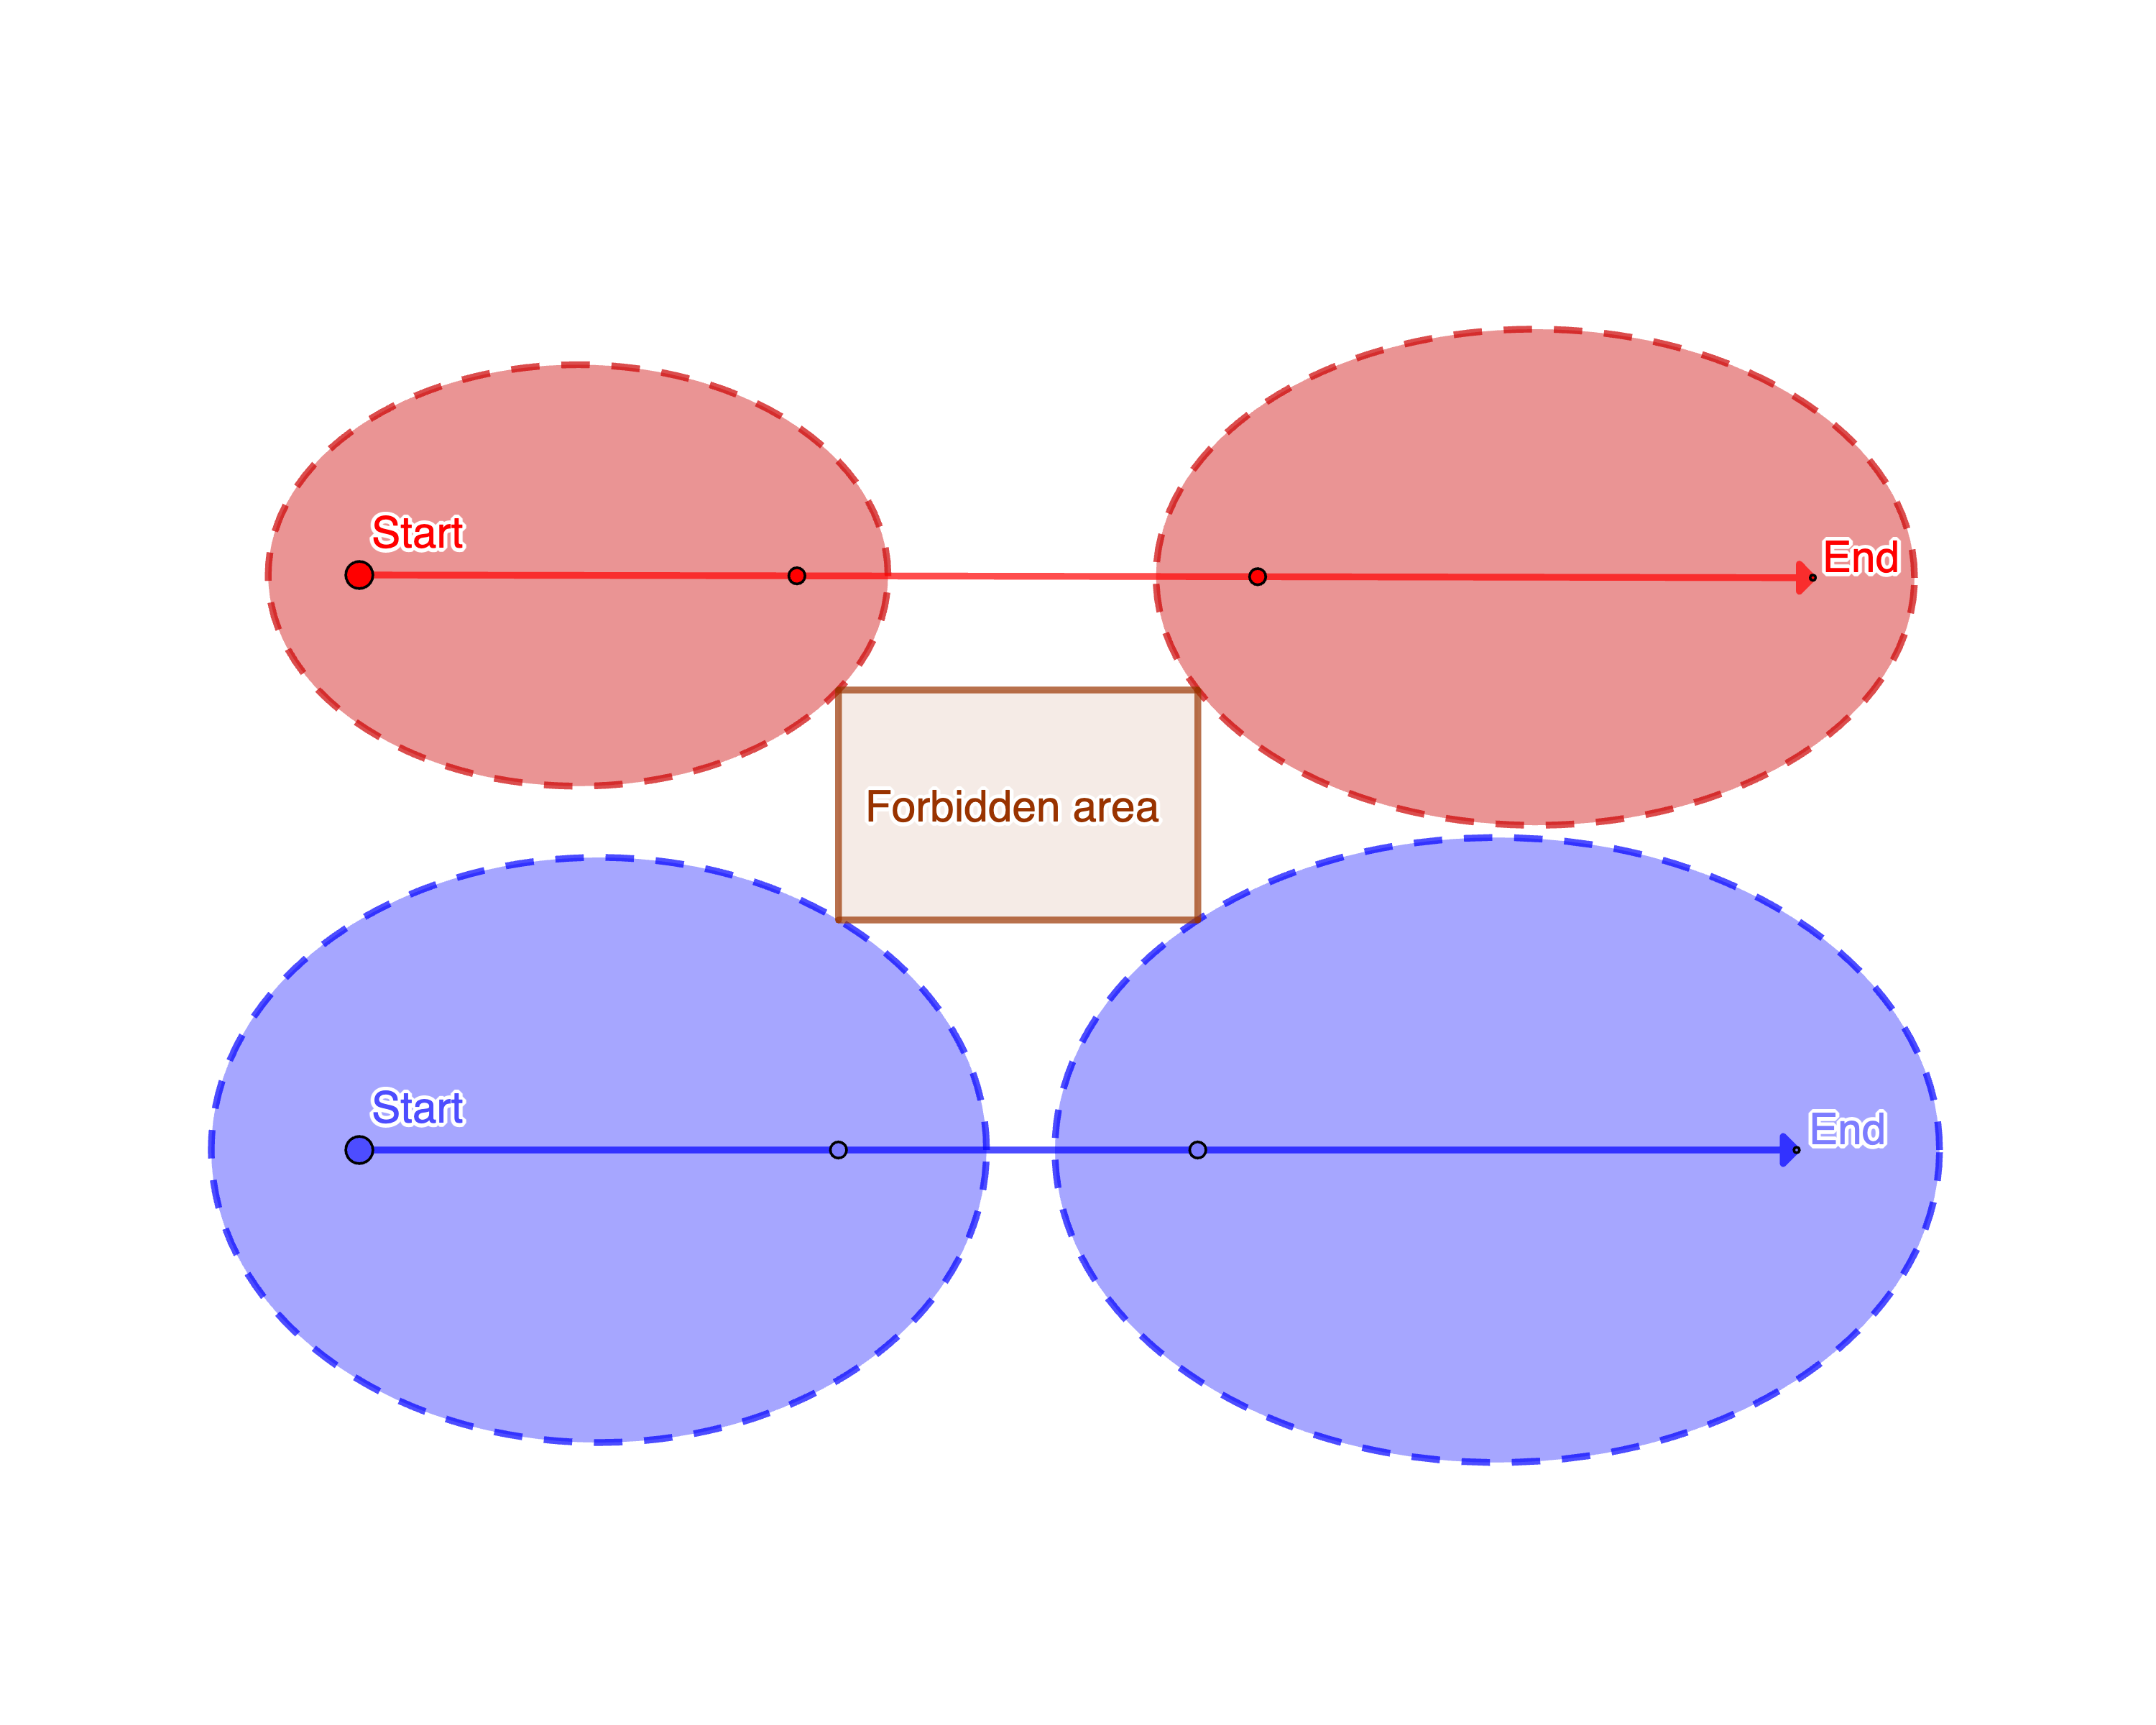
\includegraphics[width=0.45\linewidth]{SC_gen_1}}
%     \subfloat[]{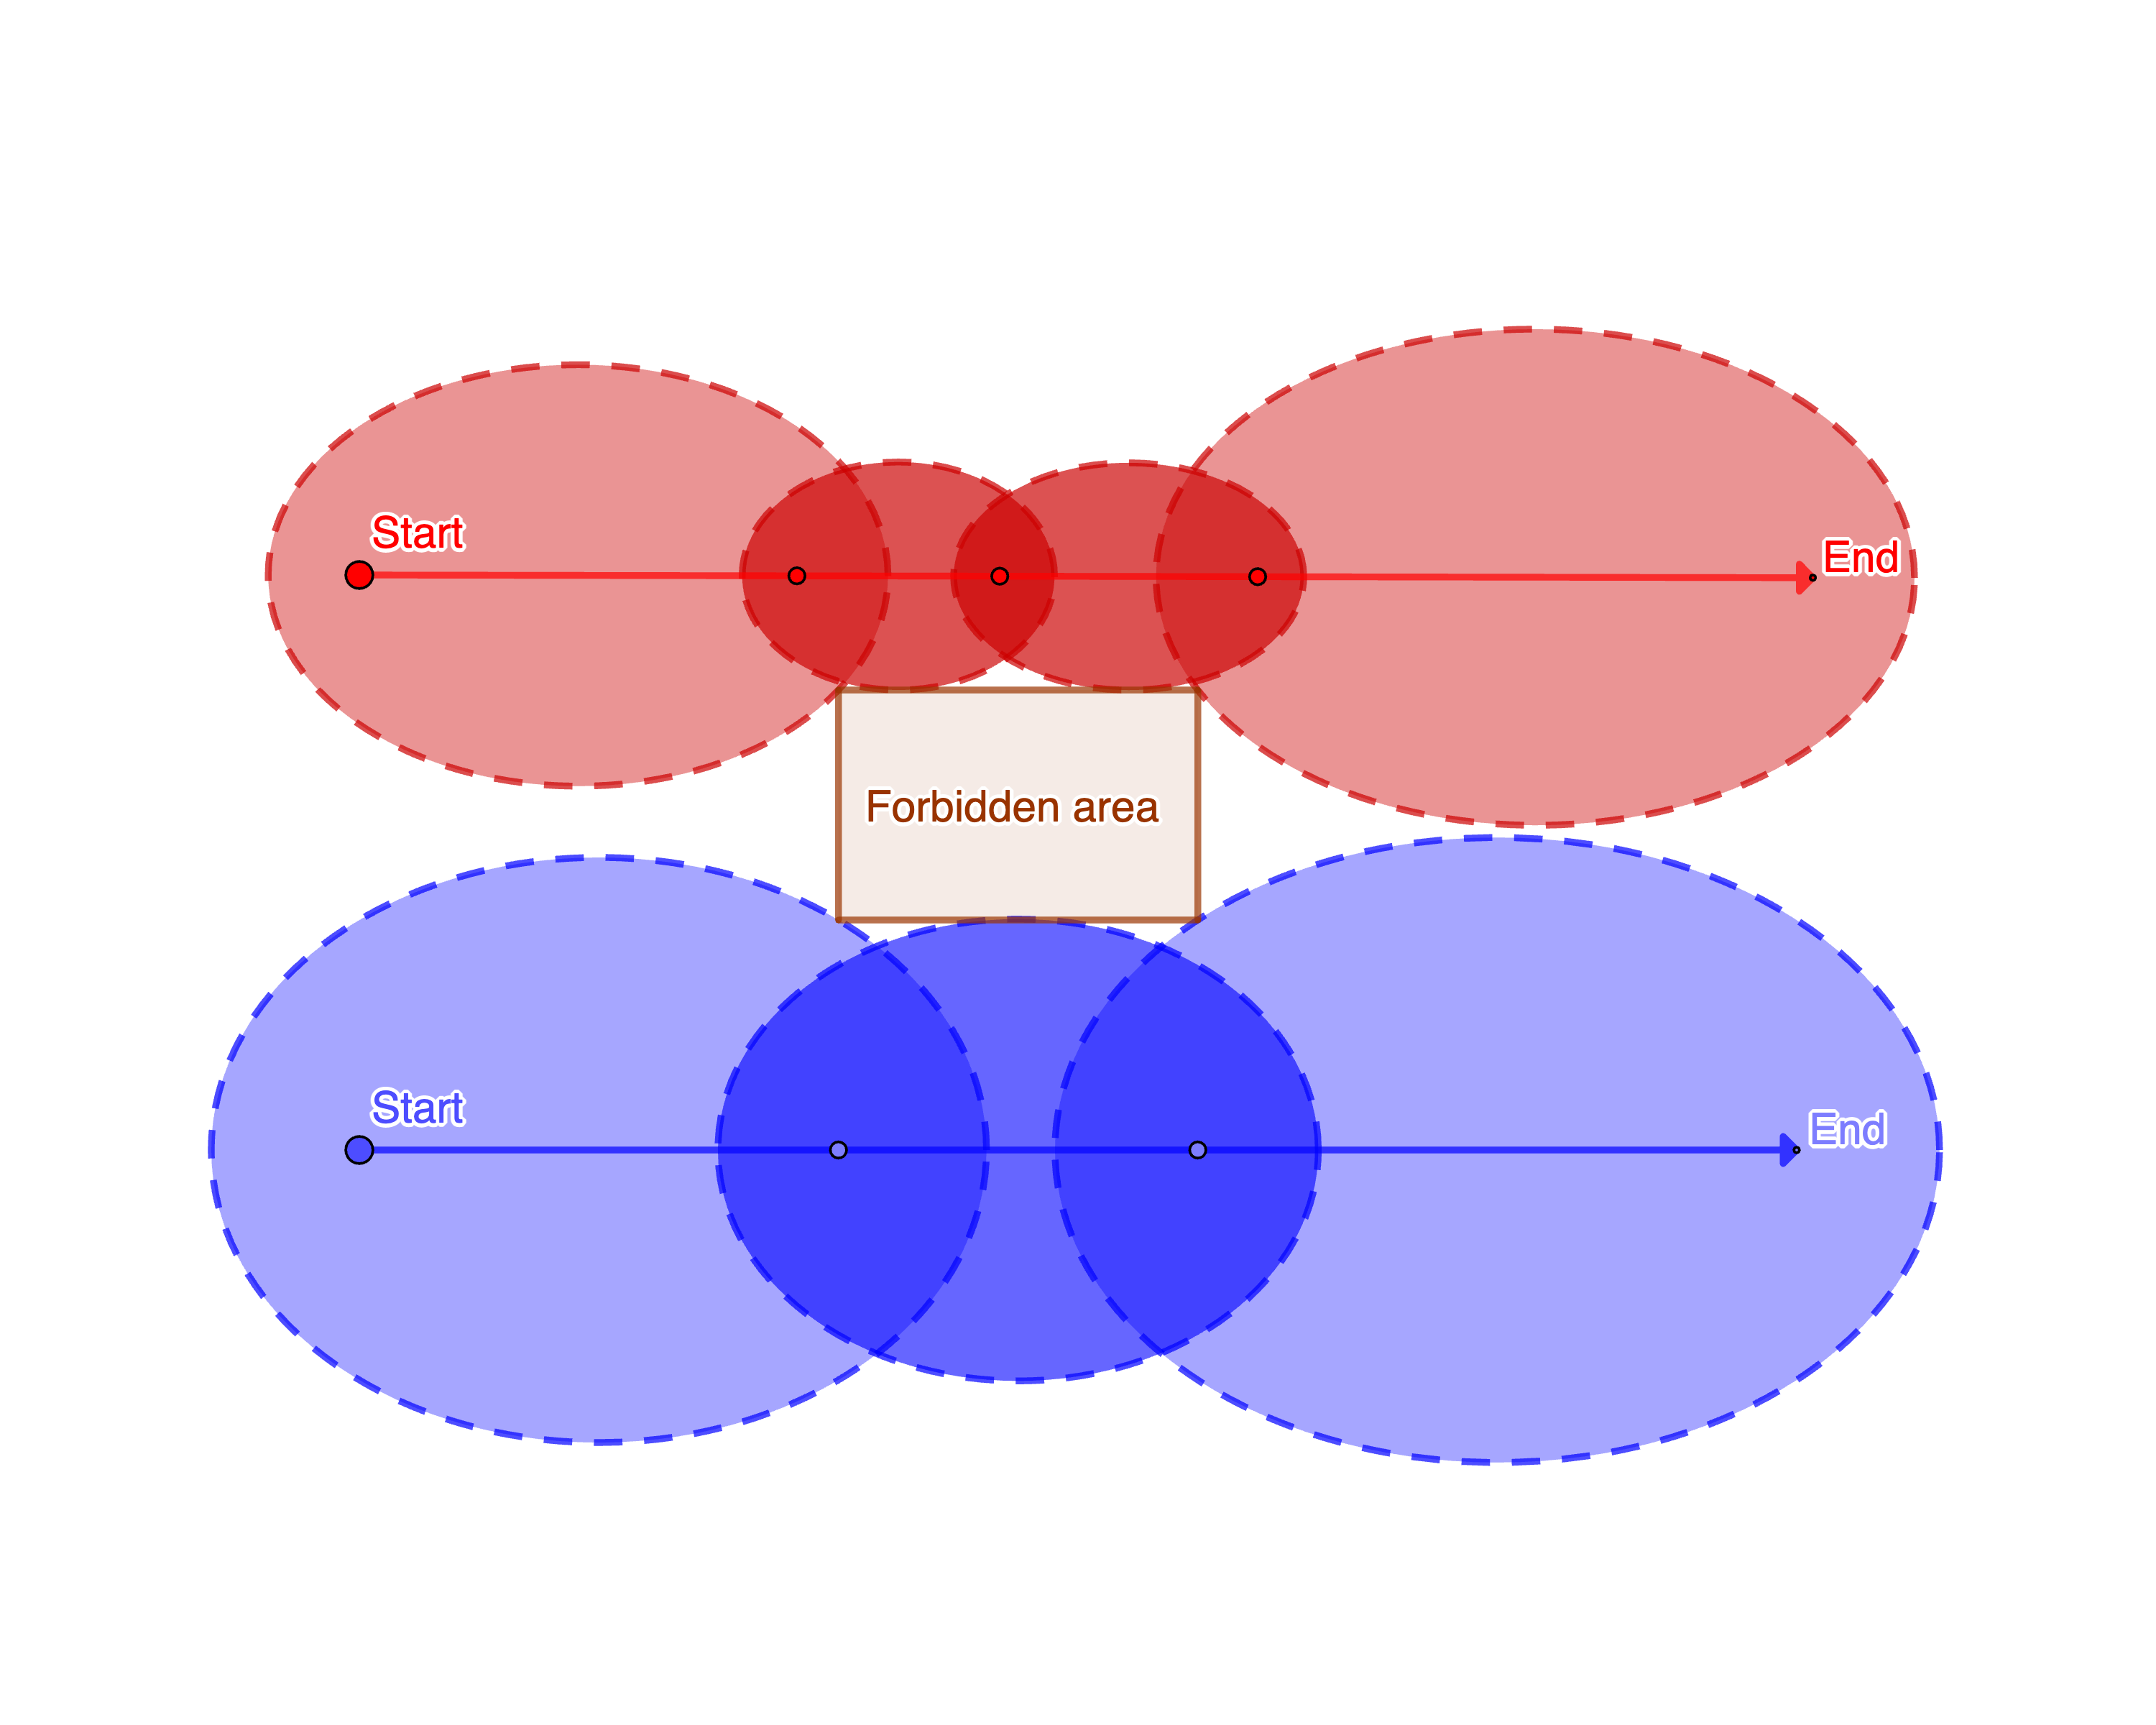
\includegraphics[width=0.45\linewidth]{SC_gen_2}}
%     \caption{Checkpoint generation example}\label{fig:checkpoint-generate}
% \end{figure}

\subsubsection{Cross-trajectory edges}\label{sec:cross-traj-edges}
To enable co-observation cross different sub-team at checkpoints, we search for available connection paths (\emph{cross-trajectory edges}) between checkpoints on different trajectories, allowing robots deviate from one sub-team to perform co-observation with a different sub-team. 
%\begin{remark}

Cross-trajectory edges $E_c = (v_1, v_2)$ define viable paths between two reference trajectories, where $\cI_{v_1}\neq\cI_{v_2}$ and at least one of $v_1 $ and $v_2$ correspond to a security checkpoint $\union_p V_p$. The cross-trajectory edges must also adhere to reachability constraints $\mathcal{E}(q_{v_1}, q_{v_2}, t_{v_1},t_{v_2}) \intersect F = \emptyset$ to ensure that no deviations into forbidden areas can occur during trajectory switches.  
%\end{remark}

\begin{figure}[htbp]
    \centering
  \subfloat[Cross-trajectory edge generation\label{fig:two-edges}]{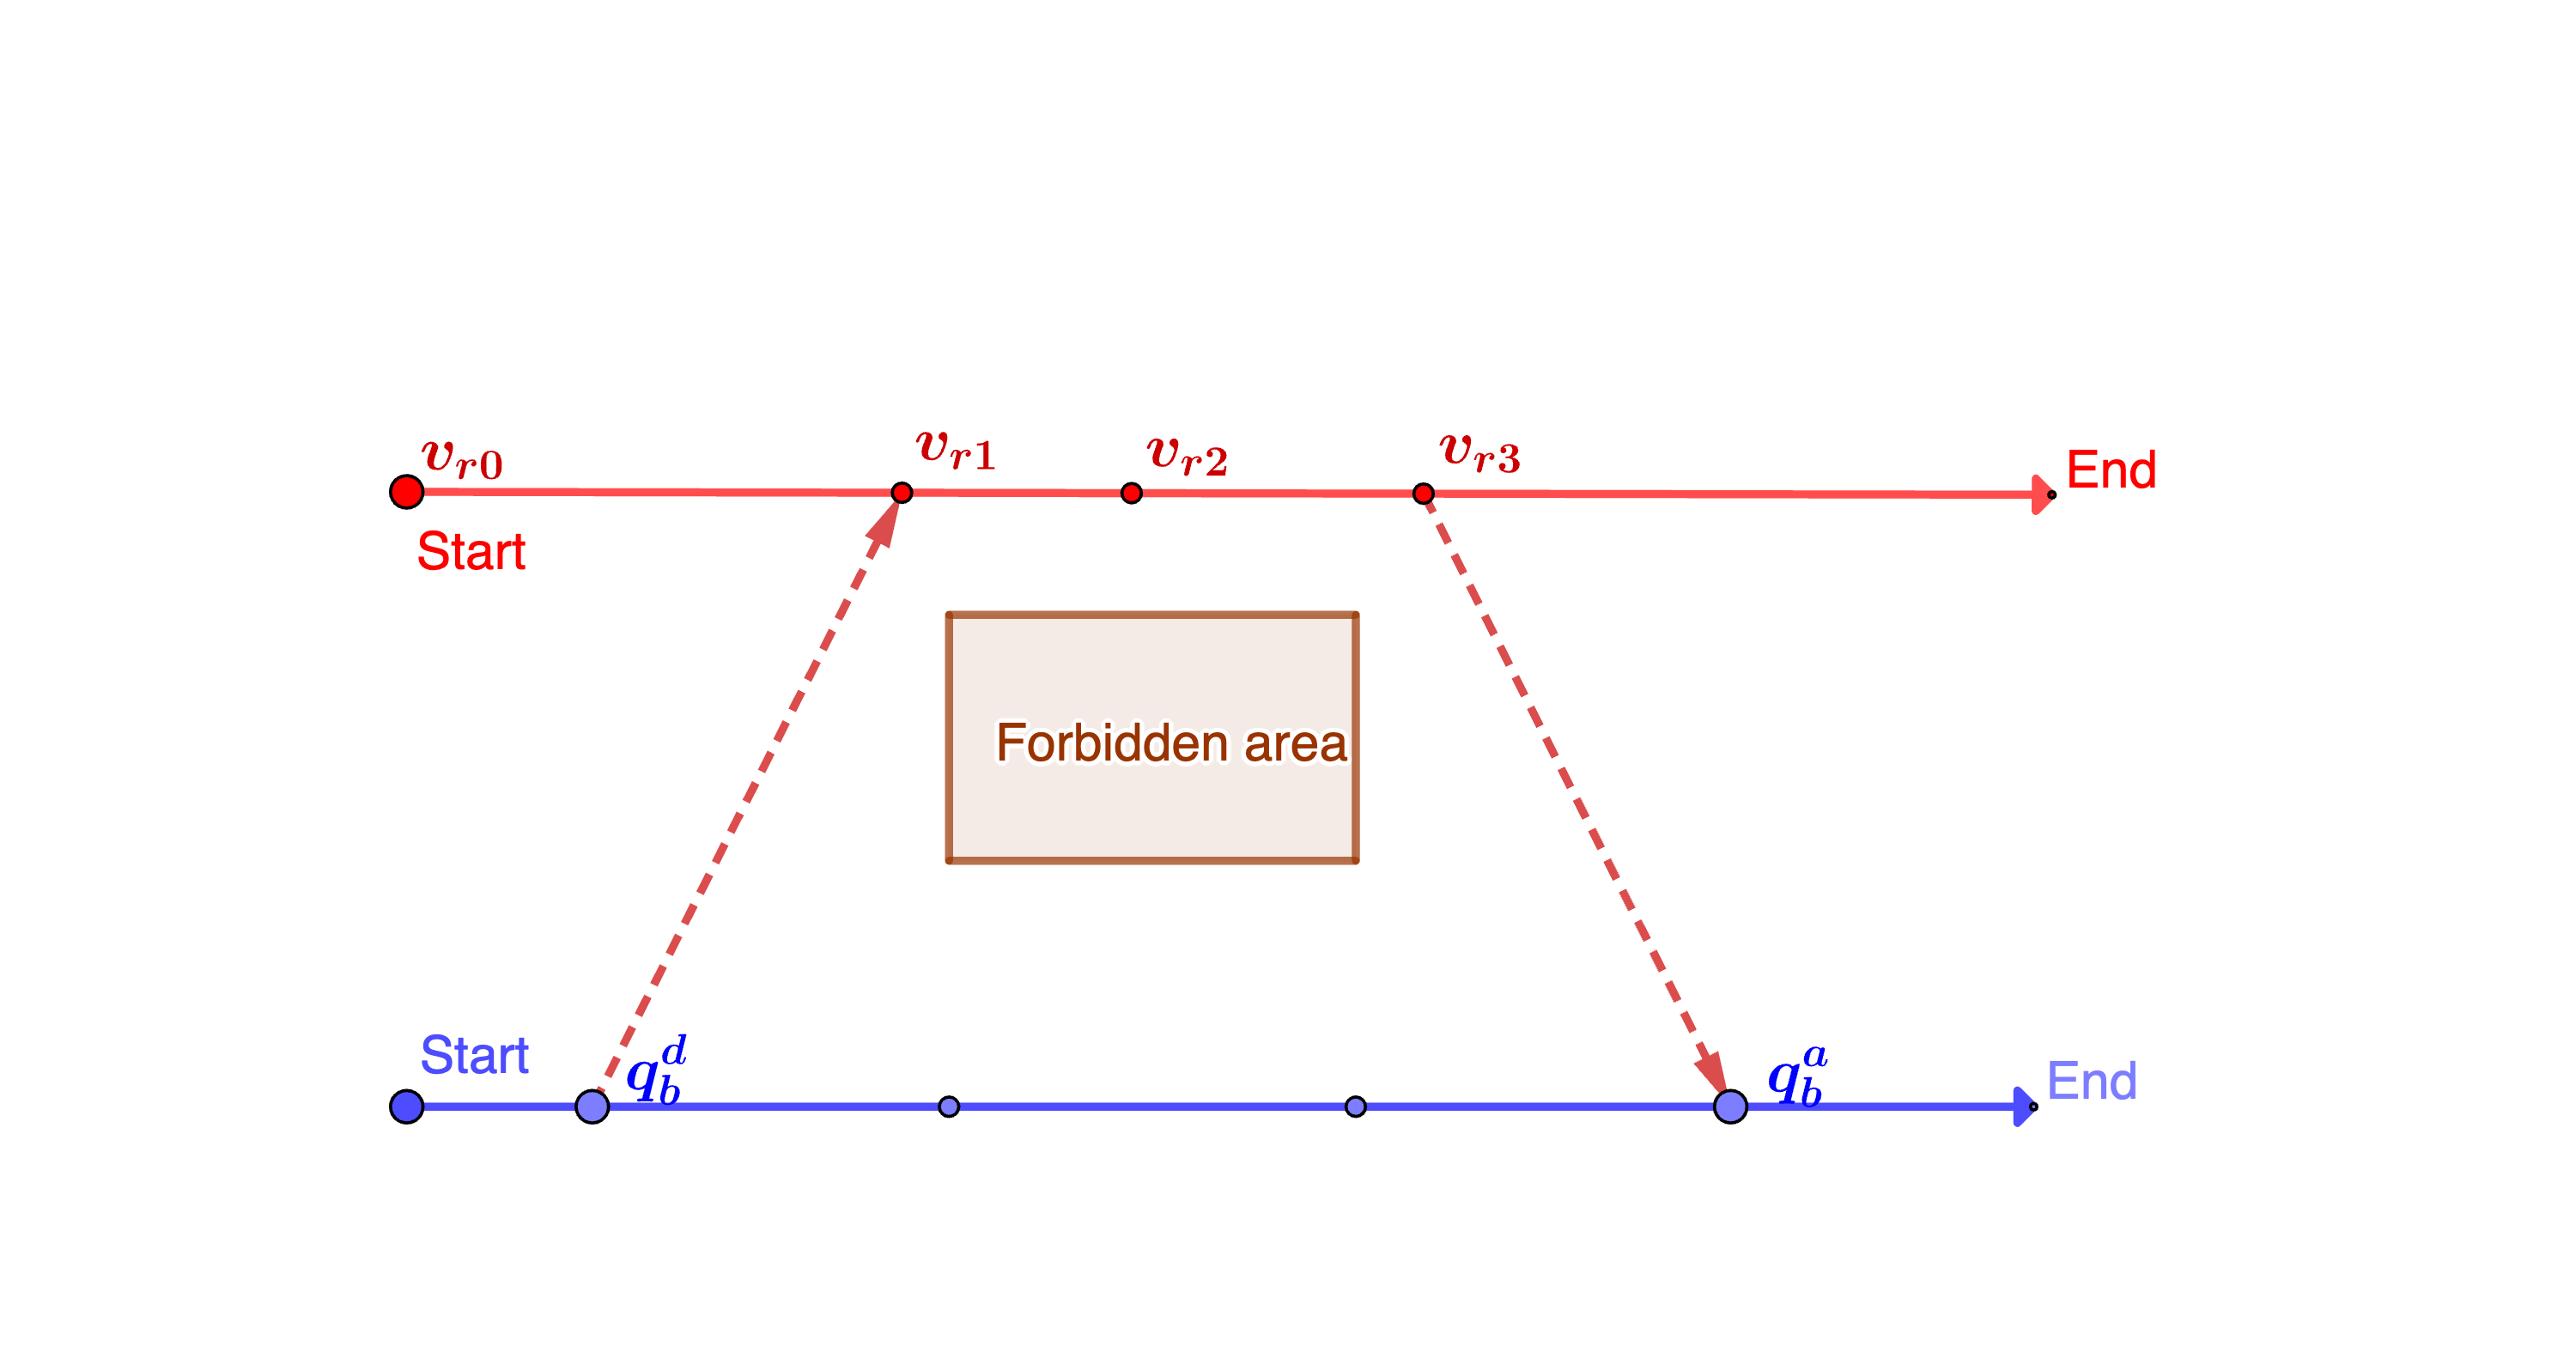
\includegraphics[width=0.45\linewidth]{two_edges}}
  \subfloat[Full checkpoint graph\label{fig:security-graph-generate}]{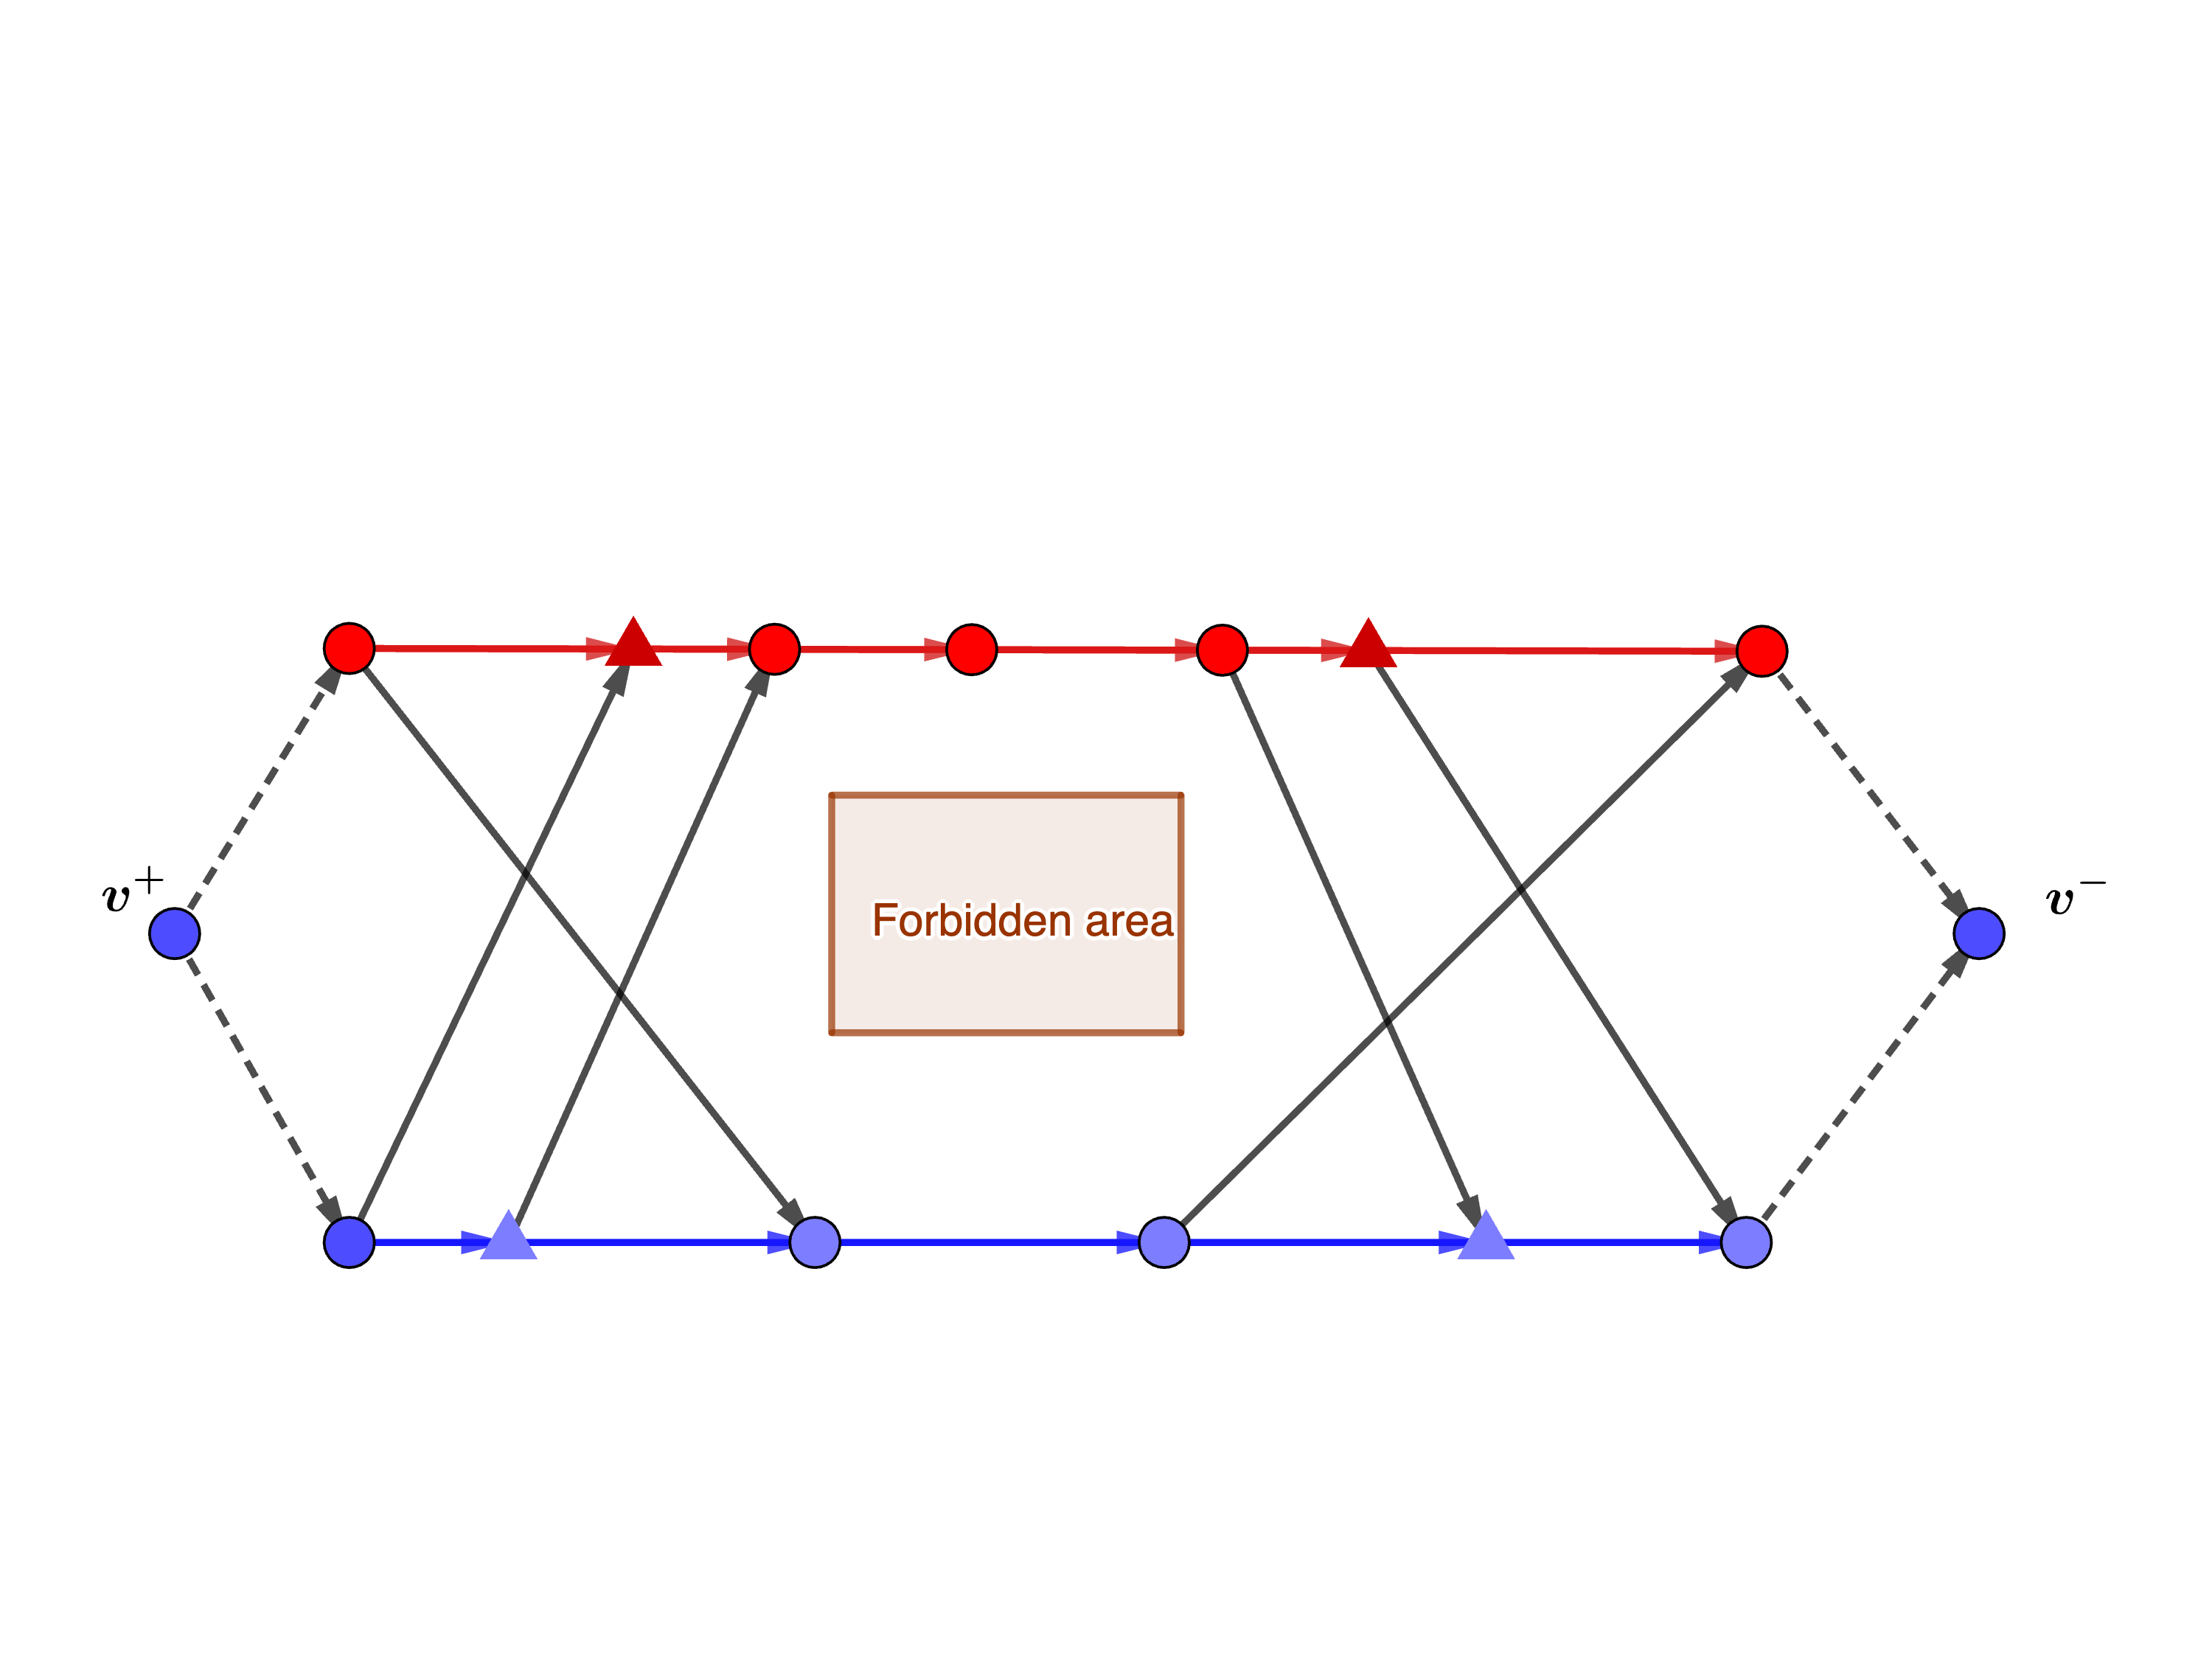
\includegraphics[width=0.45\linewidth]{security_graph}}
  \caption{\Cref{fig:two-edges}, Latest departure node $q^{d}_{b}$ found for $v_{r1}$ and earliest arrival node $q^{a}_{b}$ found for $v_{r3}$. \Cref{fig:security-graph-generate}, example of a full checkpoint graph where round vertices are checkpoint generated through the heuristic search and triangle vertices are added with the cross-trajectory edges. Virtual source $v^{+}$ and sink $v^{-}$ are added to be used later in planning problem.}  
\end{figure}

%We first find trees of feasible paths between each security checkpoint and all other trajectories using position information alone through \rrtstar{} (ignoring, for the moment, any timing constraint). Then, we prune these trees by considering time constraints (that consider the time needed to physically travel from one trajectory to the other while meeting other robots at the two endpoints) and ellipsoidal reachability constraints.

We first find trees of feasible paths between each security checkpoint and all other trajectories using position information alone (ignoring, for the moment, any timing constraint). 
More precisely, through \rrtstar{}, we find all feasible, quasi-optimal paths between one security checkpoint location $q_{v_p}(t_{v_p})$ where $v_{p} \in V_{p}$ for sub-team $\cI_p$, and all the waypoints $\{q_{r}(t_{{r}_{i}}) \}$ on any reference trajectory for a different sub-team $\cI_{r}$.
Then, to prune these trees, we consider the time needed to physically travel from one trajectory to the other while meeting other robots at the two endpoints. This is done by calculating the minimal travel time $t_{\textrm{path}}=\texttt{Cost}(q)/v_{max}$ for a robot to traverse each path. Two types of connecting nodes can be found.

\begin{description}
\item[Arrival nodes] are waypoints on $\{q_r\}$ where robots from sub-team $\cI_p$, deviating at $v_p$, can meet with sub-team $\cI_r$ at $(q_r(t_{r_i}),t_{r_i})$. For these, \rrtstar{} must have found a path from $v_p$ to $q_{r}(t^{a}_r)$ with $t_{p}+t_{\textrm{path}}<t_{{r}_{i}}$, and $\mathcal{E}(q_{r}(t_{{r}_{i}}),q_{p},t_{{r}_{i}},t_{p}) \intersect F = \emptyset$.

For each trajectory $r\neq p$, we define the \emph{earliest arrival node} from $v_p$ to $v_{ea} = (q_{r}(t^{a}_r),t^{a}_r)$ as the arrival node characterized by the minimum $t^{a}_r$ discovered. 
%$t^{a}_r$ is designated as the \emph{earliest arrival time}.

\item[Departure nodes] are the waypoints on $\{q_r\}$ such that a robot from sub-team $\cI_r$, deviating from $(q_{r}(t_{{r}_{i}}),t_{{r}_{i}})$, can meet with robots in sub-team $\cI_p$ at $v_{p}$. For these nodes, \rrtstar{} must find a path from $v_p$ to $q_{r}(t_{{r}_{i}})$ for $v_p$ if  $t_{p}>t_{{r}_{i}}+t_{\textrm{path}}$ and $\mathcal{E}(q_{p}, q_{r}(t_{{r}_{i}}),t_{p}, t_{{r}_{i}}) \intersect F = \emptyset$. 

For each trajectory $r\neq p$, we define the \emph{latest departure node} $v_{ld}=(q_{r}(t^{d}_r),t^{d}_r)$ as the departure node characterized by the maximum $t^{d}_r$ discovered.
% $t^{d}_r$ is designated as the \emph{latest departure time}.
\end{description}

For each $v_{p} \in V_{p}$ found through \Cref{alg:checkpoint-gen}, all the latest departure and earliest arrival nodes are added as vertices $V_q = V_{p} \union \{v_{ea}, v_{ld}\}$, and the corresponding paths are added as cross-trajectory edges to $E_{q}$. Examples are shown in Figure \ref{fig:two-edges}.

\subsubsection{In-trajectory edges}\label{sec:Graph-intro}

%With vertices $V_{q}$ and cross-trajectory edges $E_{q}$ found in Algorithm \ref{alg:cross-trajectory-edges}, we can construct a security graph $G_{q}$. 
We arrange all $V_q =\union_p \{v^0_{p}, \dots ,v^T_{p}\}$ found in \Cref{sec:security-checkpoint,sec:cross-traj-edges} in ascending order of $t_{v^i_{p}}$. We then add to $E_q$ the \emph{in-trajectory edges} $\{(v^i_{p}\rightarrow v^{i+1}_{p})\}$ obtained by connecting all consecutive checkpoints $v^i_{p}\in V_q$ with the checkpoints $v^{i+1}_{p}$ that follow them in their original trajectories. Examples are shown in Figure \ref{fig:security-graph-generate}. %\zyang{any better explaination?}

%For convenience, we use $|V_{q}|$ and $|E_{q}|$ to denote the cardinality of the sets $V_{q}$ and $E_{q}$ 

\subsection{Co-observation planning problem}
In this section, we formulate the cross-trajectory planning problem as a network multi-flow problem, and solve it using mixed-integer linear programs (MILP). We assume that $n_p$ robots are dedicated (one in each sub-team) to follow the reference trajectory (named \emph{reference robots}). The goal is to plan the routes of the $n-n_p$ additional \emph{cross-trajectory robots} dedicated to cross-trajectory co-observations, and potentially minimize the number of ross-trajectory robots needed. 

\begin{remark}
Note that we assign fixed roles to robots for convenience in explaining the multi-flow formulation. In practice, after a cross-trajectory robot joins a team, it is considered interchangable, and could switch roles with the reference robot of that trajectory. % (i.e., the original reference robot might serve as a cross-trajectory robot in a later cross-trajectory co-observation).
\end{remark}

To formulate the problem as a network multi-flow problem, we augment the checkpoint graph $G_{q}$ to a flow graph $G=(V, E)$. The vertices of the new graph $G$ are defined as $V= V_{q} \union \{v^{+},v^{-}\}$, where $v^{+}$ is a \emph{virtual source} node, and $v^{-}$ is a \emph{virtual sink} node. We add directed edges from $v^{+}$ to all the start vertices, and from all end vertices to $v^{-}$, with $v^0_p$ and $v^T_p$ representing the start and end vertices of sub-team $\cI_p$. The edges of the new graph are defined as $E = E_{q} \union \{(v_{+},v^{0}_{p})\}_{p} \union \{( v^{T}_{p},v_{-})\}_{p}$.

%The goal is to find paths in $G$ for all the cross-trajectory robots that starts from the virtual source $v^{+}$ and ends in the virtual sink $v^{-}$.
The path of a robot $k$ all starts from $v^{+}$ and ends at $v^{-}$, and are represented as a flow vector $\vf^{k} = \{ f^{k}_{ij} \}$, where $f^{k}_{ij} \in \{1,0\}$ is an indicator variable representing whether robot $k$'s path contains the edge $v_{i}\to v_{j}$. The planning problem can be formulated as a path cover problem on $G_{q}$, i.e., as finding a set of paths $F=[\vf_{1},\dots, \vf_{\cK}]$ for cross-trajectory robots such that every checkpoint in $\union_p V_{p}$ is included in at least one path in $F$ (to ensure co-observation at every checkpoint as required by \Cref{rmk:revised-security}). %Additionally, to encourage the robots' exchange between different sub-teams, cross-trajectory co-observations should be preferred compared to co-observation within the same team. 

Technically, we can always create a trivial schedule that involves only co-observations between members of the same team; this, however, would make the solution more vulnerable in the case where multiple agents are compromised in the same team. While in this paper we explicitly consider only the single attacker scenario, multi-attacks can be potentially handled by taking advantage of the \emph{decentralized blocklist protocol} introduced in \cite{wardega2023byzantine}. For this reason, we setup the methods presented below to always prefer \emph{cross-trajectory co-observation} when feasible.

Finally, edges from the virtual source and to the virtual sink should have zero cost, to allow robots to automatically get assigned to the starting point that is most convenient for the overall solution (lower cost when taking cross-trajectory edges).
These requirements are achieved with the weights for edges $(v_{i},v_{j})\in E$ defined as:
\begin{equation}
	w_{i,j}=\begin{cases}
	-w_{t} & \cI_{v_{i}}=\cI_{v_{j}}, (v_{i},v_{j})\in E_{q}\\
	w_{c} & \cI_{v_{i}} \neq \cI_{v_{j}}, (v_{i},v_{j})\in E_{q}\\
	0 &  (v_{i},v_{j})\in E / E_{q} 
	\end{cases}
\end{equation}
where $w_{c} > w_{t}$. 

With the formulation, the planning problem is written as an optimization problem, where the optimization cost balances between the co-observation performance and total number of flows (cross-trajectory robots) needed:
 \begin{subequations} \label{eq:flow-coverage-problem}
     \begin{align}
        \min_{F} &\sum^{\cK}_{k} \sum_{(+i)\in E} f^{k}_{+i} - \rho \sum^{\cK}_k \sum_{(ij)\in E} w_{ij} f^k_{ij} \label{eq:flow-cost}\\
        s.t. & \sum_{\{h:(hi) \in E\}}f^k_{hi}=\sum_{\{j:(ij) \in E\}}f^k_{ij},  \forall k,\forall v \in V_{q} / \{v^{+}, v^{-}\}  \label{eq:FlowBalanceConstraint}\\
        & \sum^{\cK}_k\sum_{\{i:(ij)\in E \}} f^k_{ij} \geq 1, \forall v_{j} \in \{V^{s}_{p}\} \label{eq:FlowCoverage}\\
        & f^k_{ij} \in \{0,1\} \,  \forall (ij)\in E\label{eq:SingleFLowCapacity}
     \end{align}
 \end{subequations}
where, for convenience, we used $(ij)$ to represent the edge $(v_{i},v_{j})$, and $(+i)$ to represent the edge $(v^{+},v_{i})$.

The first term in the cost \eqref{eq:flow-cost} represents the total number of robot used, and the second term represents the overall co-observation performance (defined as the total number of cross-trajectory edges taken by all flows beyond the regular trajectory edges); the constant $\rho$ is a manually selected penalty parameter to balance between the two terms. \eqref{eq:FlowBalanceConstraint} is the flow conservation constraint to ensures that the amount of flow entering and leaving a given node $v$ is equal (except for $v^{+}$ and $v^{-}$). \eqref{eq:FlowCoverage} is the flow coverage constraints to ensures that all security checkpoints $ \{V^{s}_{p}\}$ have been visited co-observed. The security graph $G_{q}$ is acyclic, making this problem in complexity class $P$, thus, can be solved in polynominal time \cite{1702662}. 

\subsection{Co-observation performance}
Notice that problem \eqref{eq:flow-coverage-problem} is guaranteed to have a solution for $\cK=N_{p}$ where all $\cK$ robots follows the reference trajectory ($f^{k}_{ij}=1, \forall \cI_{v_{i}}=\cI_{v_{j}}=k$).  %Additionally, for a fixed number of robots $\cK \geq N_{p}$, 
It is possible for the resulting flows to have a subset of flows $F_{e} \in F$ that is empty, i.e. $f_{ij}=0, \forall (v_{i},v_{j})\in E$, $f\in F_{e}$; these flow will not increase the cost and can be discarded from the solution.  

The constant $\rho$ selects the trade-off between the number of surveillance robots and security performance. An increase in robots generally enhancing security via cross-trajectory co-observations; this also increases the complexity of the coordination across robots. In order to identify the minimum number of robots necessary, we propose an iterative approach where we start with $\cK=1$ and gradually increases it until $F$ contains an empty flow, indicating the point where further robot additions do not improve performance. 

\begin{remark} 
The value of row $\rho$ is upper bounded such that the second term for each single flow in \eqref{eq:flow-cost} is always smaller than one, i.e., $ \rho \sum_{(ij)\in E} w_{ij} f^k_{ij}\leq 1$. Otherwise, the iteration continues indefinitely as adding additional flow introduce a negative term $\sum_{(+i)\in E} f^{k}_{+i} - \rho\sum_{(ij)\in E} w_{ij} f^k_{ij} = 1- \rho\sum_{(ij)\in E} w_{ij} f^k_{ij}<0$ which always makes the cost \eqref{eq:flow-cost} smaller.
\end{remark}

\subsection{Result and simulation}

\begin{figure}
  \centering
  \subfloat[Cross-trajectory co-observation plan \label{fig:previous_result_plan}]{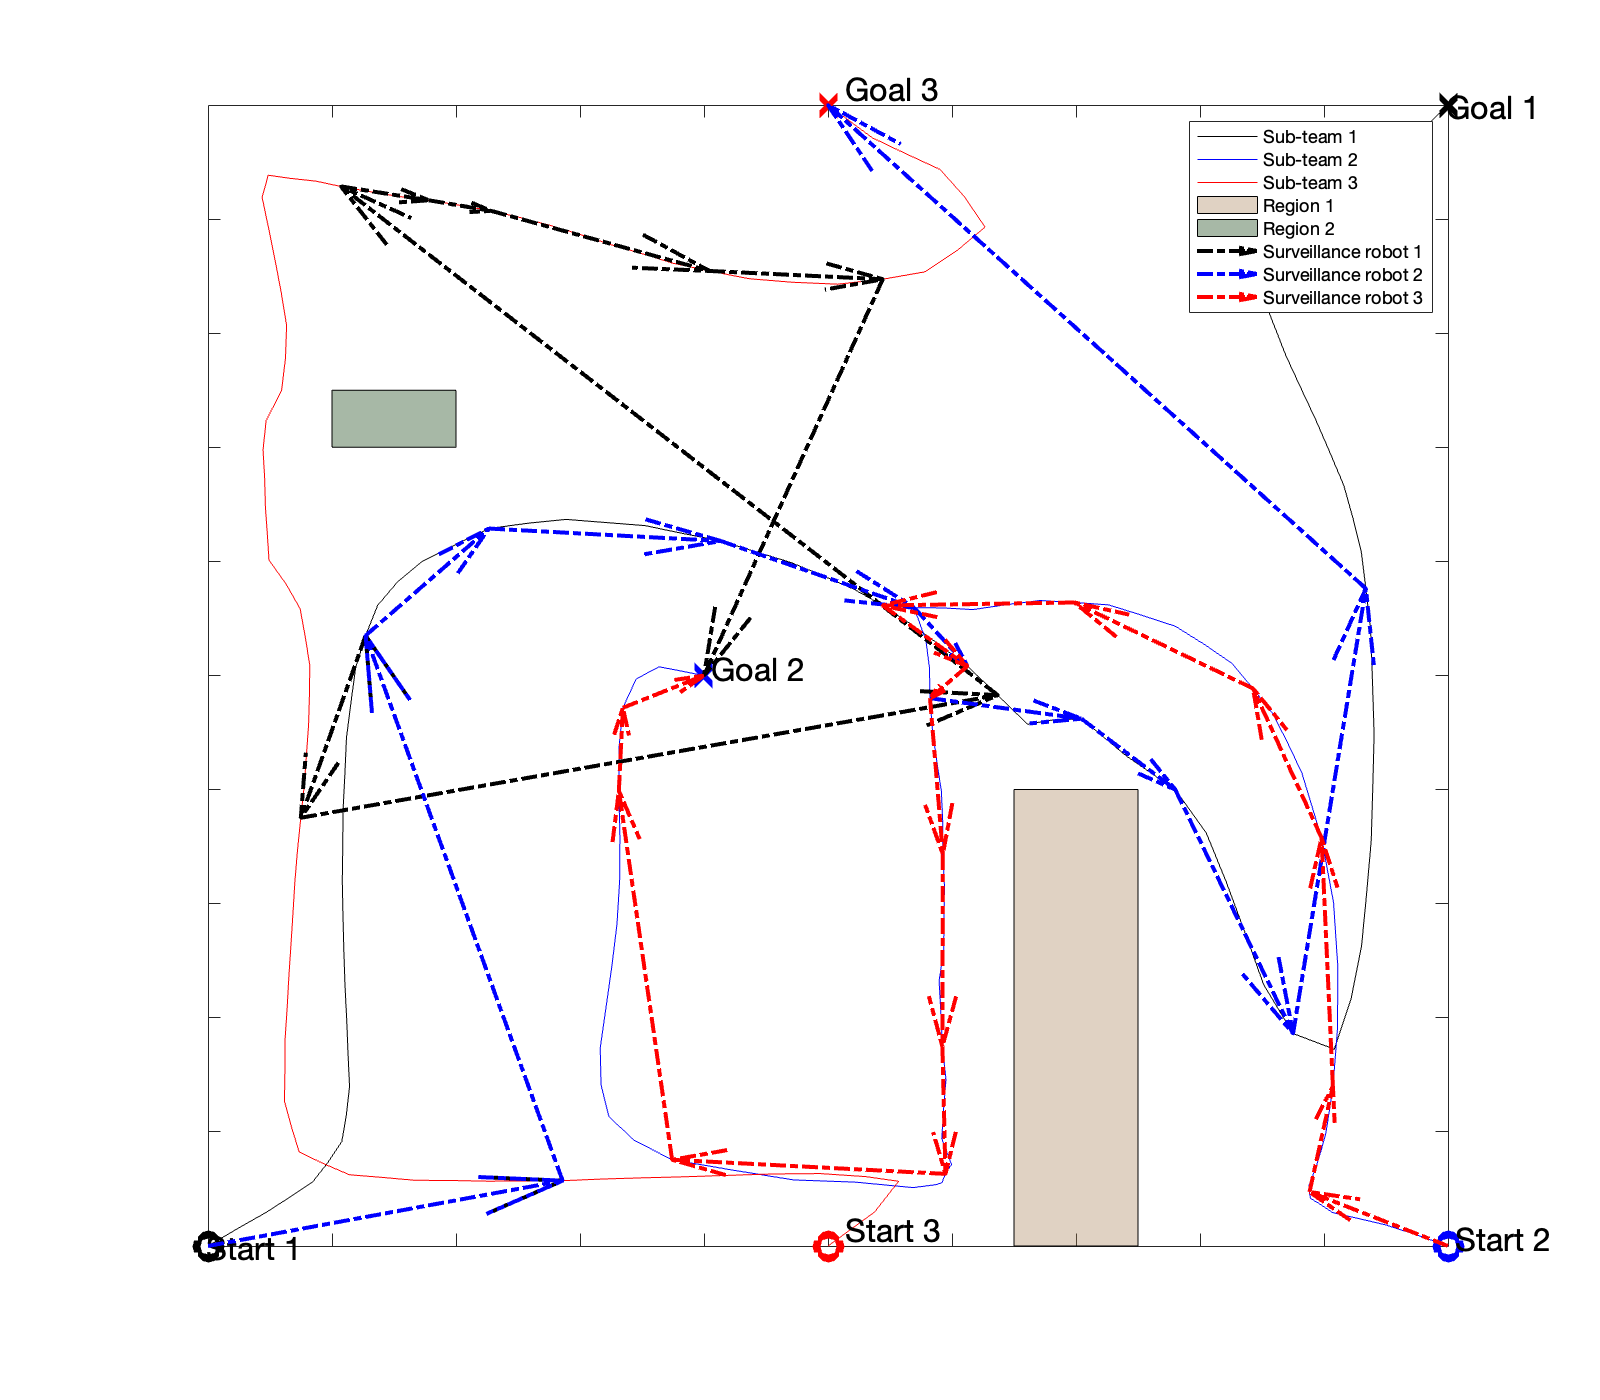
\includegraphics[width=0.47\linewidth, trim = 4cm 2cm 4cm 2cm,valign=c]{old_result}}
  \subfloat[Checkpoint graph and result flows \label{fig:previous_result_graph}]{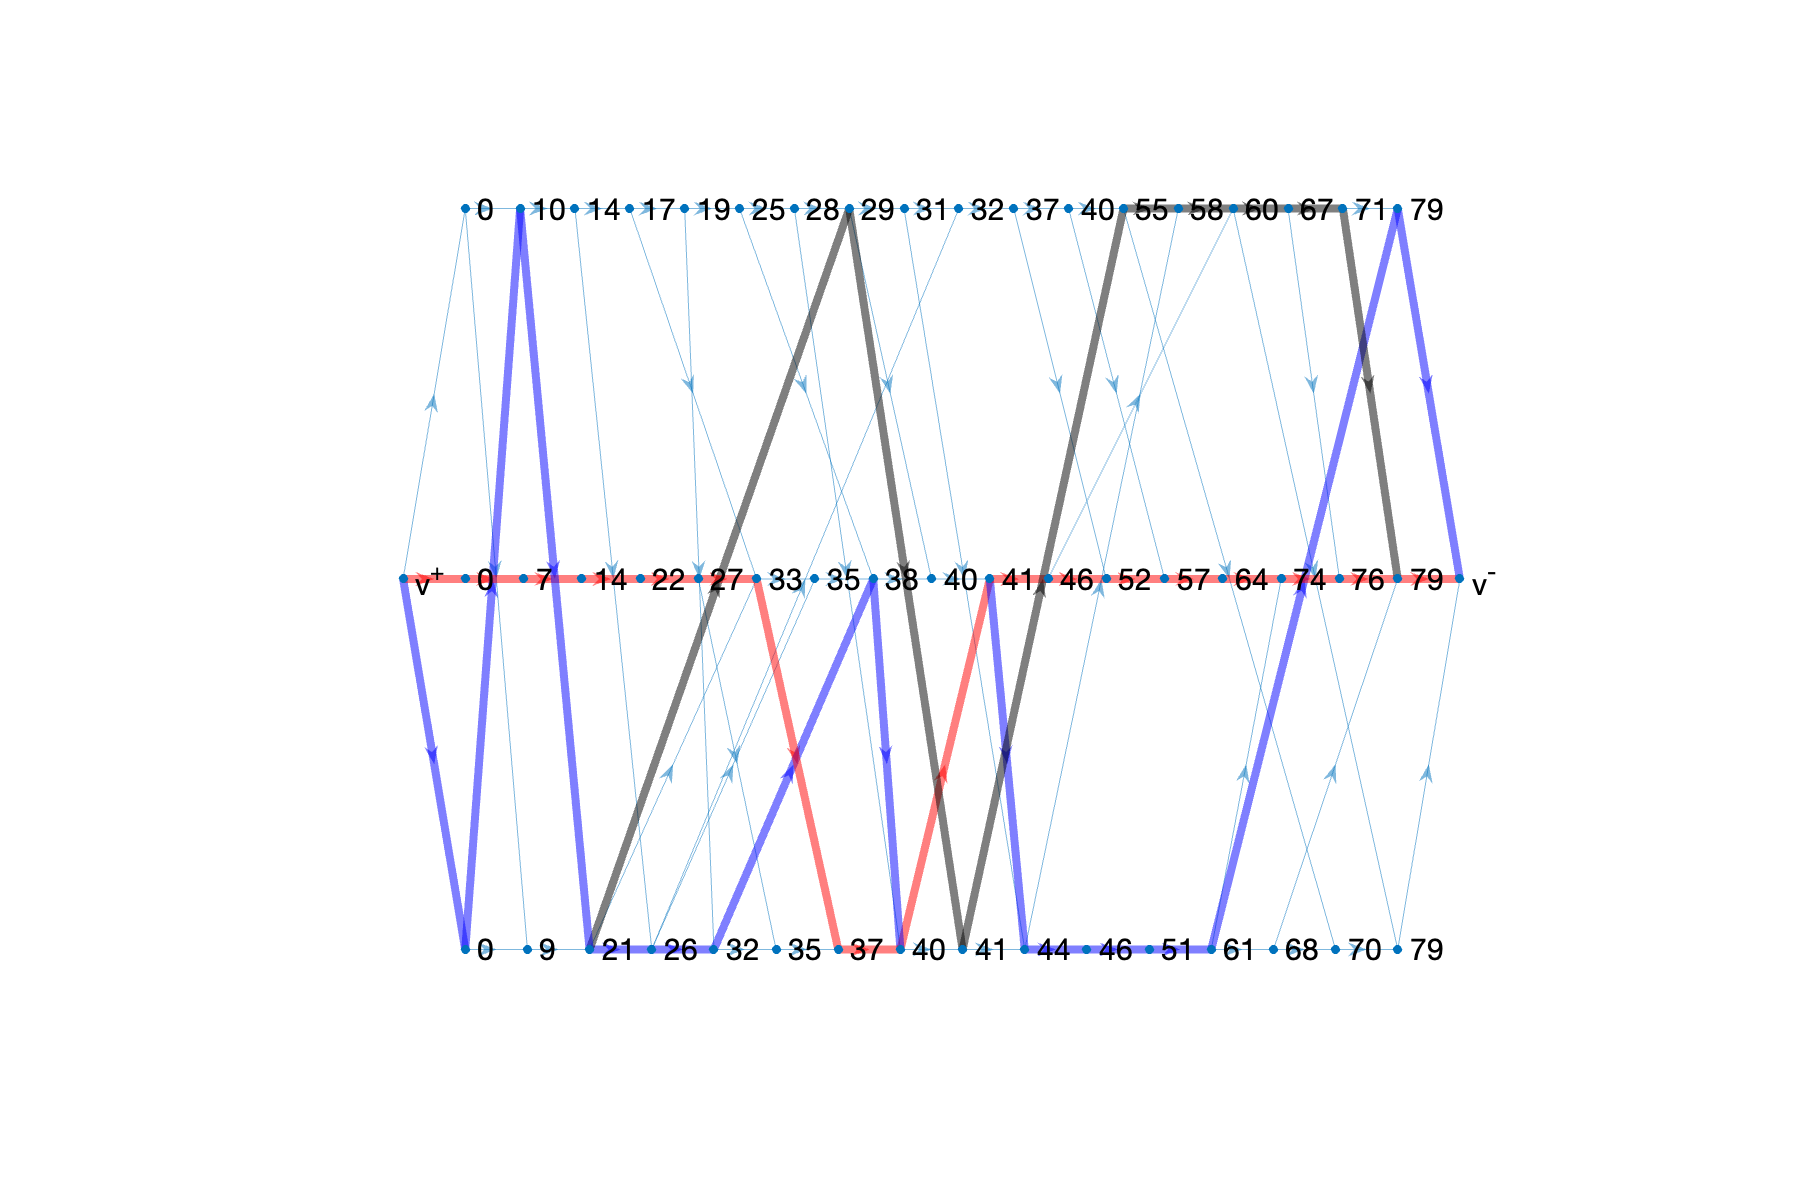
\includegraphics[width=0.47\linewidth, trim = 4cm 1cm 4cm 1cm,valign=c]{old_result_graph.png}}
  \caption{\Cref{fig:previous_result_plan} showcase an unsecured 4-robot map exploration task. The cross-trajectory co-observation plan is shown as dotted arrors on top of the original plan in \Cref{fig:previous_result_plan}. The checkpoint graph and resulting flows are shown in \Cref{fig:previous_result_graph}.}
  \label{fig:3-team-ctco}
\end{figure}

We first test the proposed method for the example application in \Cref{fig:example-application,fig:ReachabilitySimulation}, using the same setup in \Cref{sec:ADMM-simulation}. Using the parameters $w_{c}=10$, $w_{t}=1$ and $\rho = 0.01$, the result returns a total of $\cK=3$ surveillance robots with cross-trajectory plan shown in \Cref{fig:3-team-ctco}. %In \Cref{fig:previous_result_grap}, each horizontal line represents the original trajectory of a sub-team and the number on each vertex $v_{i}$ represents the corresponding time $t_{i}$. 
The flows derived from the solution of the optimization problem \eqref{eq:flow-coverage-problem} are highlighted in the graph \Cref{fig:previous_result_graph}, where each horizontal line represents the original trajectory of a sub-team and the number on each vertex $v_{i}$ represents the corresponding time $t_{i}$. The planning result in the workspace is shown in \Cref{fig:previous_result_plan} as dash-dotted arrows with the same color used for each flow in \Cref{fig:previous_result_graph}. Compared with the result in \Cref{fig:ReachabilitySimulation}, it is easy to see that there is a significant improvement in map coverage in \Cref{fig:previous_result_plan}. At the same time, unsecured deviations to the forbidden regions of robots are secured through cross-trajectory observations. 

The problem shows no solution for $\cK\leq 2$. For cases $\cK=3$, problem return the optimal result as shown in \Cref{fig:Cross-trajectory-result}. If we further increase $\cK>3$, we do not get a better result; instead, the planner will return four flows with the rest $\cK-3$ flows empty. 

We then test the proposed method for a 4-team and 7-team case with result shown in Figure \ref{fig:Cross-trajectory-result}, where four trajectories are provided for a map exploration task with no security related constraints (co-observation schedule and reachability). We have a $10m\times10m$ task space, three forbidden regions (rectangle regions in \Cref{fig:Result-plan}) and robots with a max velocity of $0.5m/dt$. 

\begin{figure}
  \centering
  %\subfloat[Unsecured plan\label{fig:unsecured-plan}]{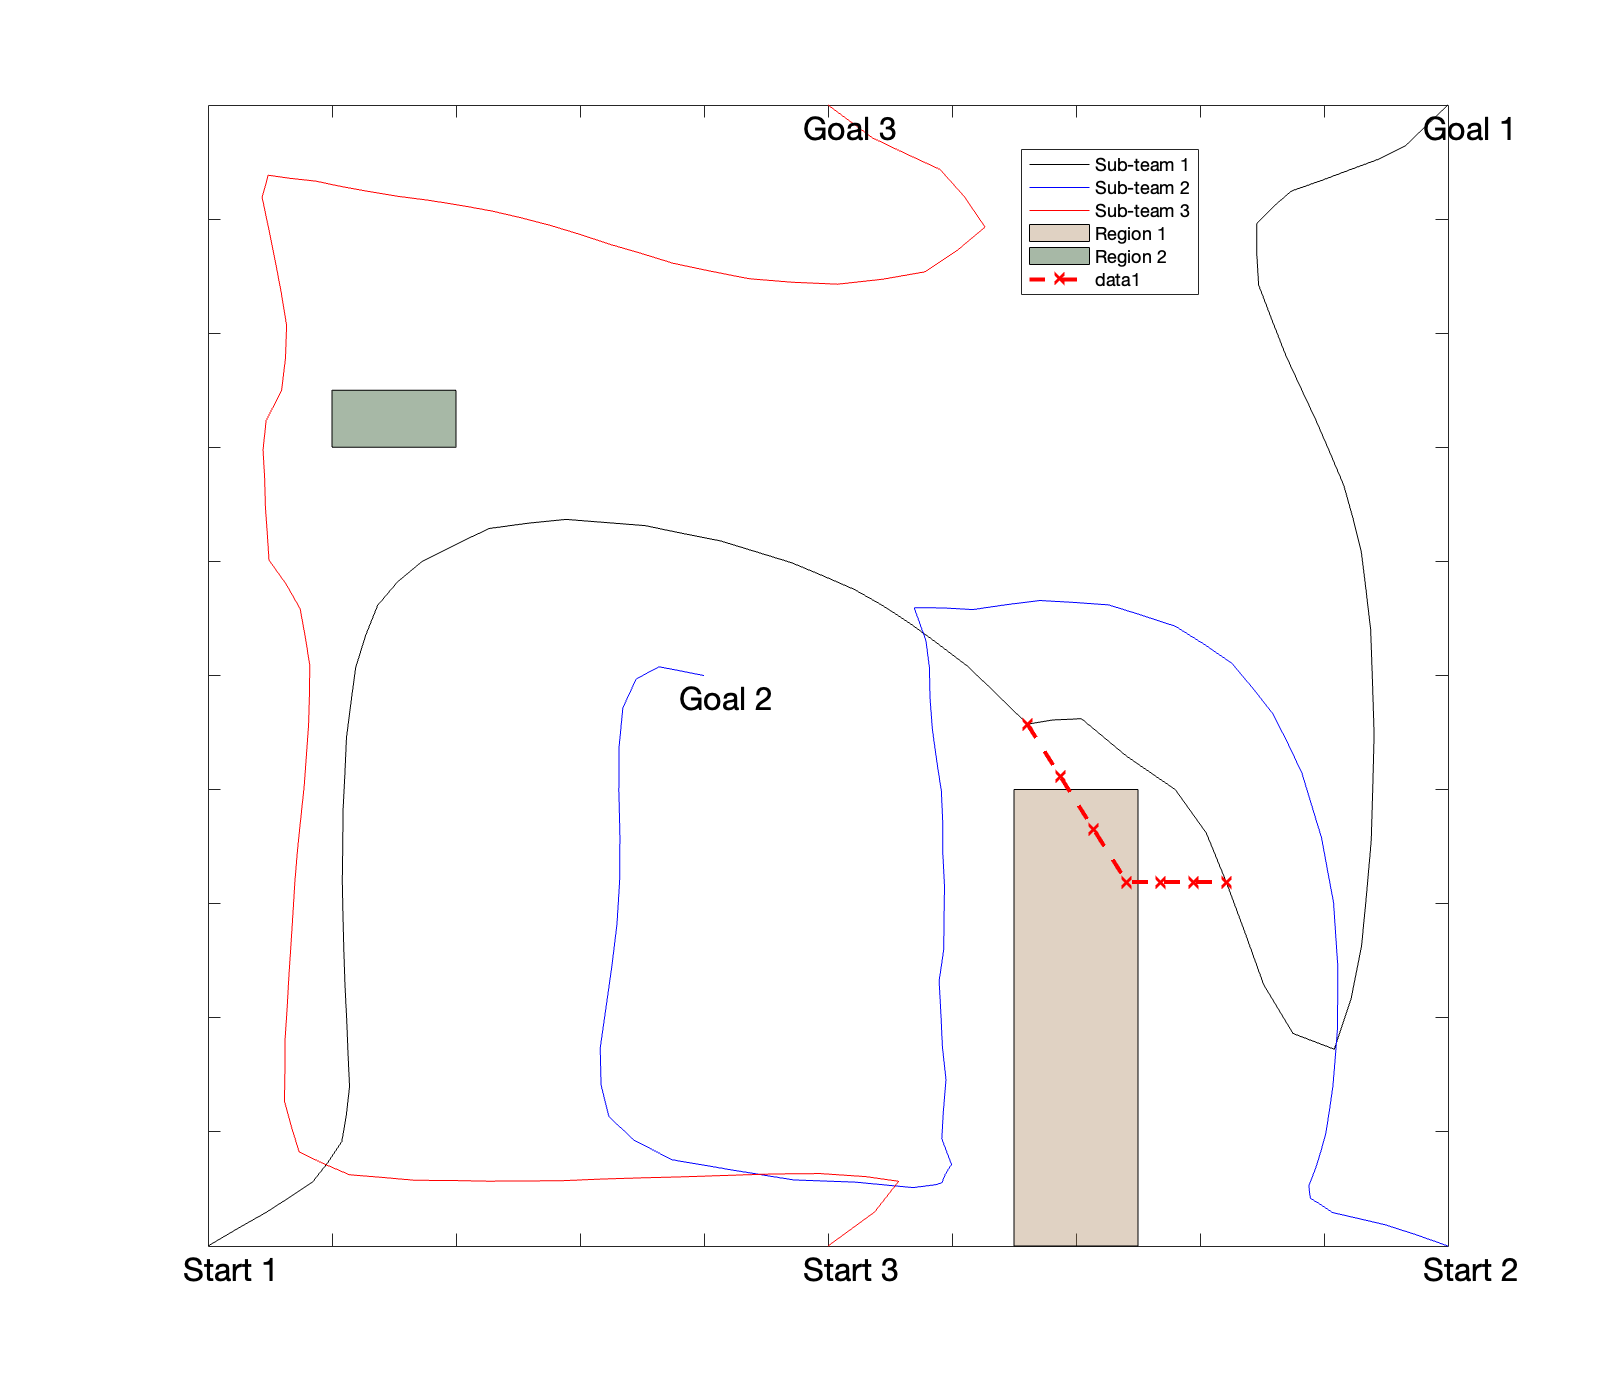
\includegraphics[width=0.31\linewidth, trim = 3cm 2cm 3cm 2cm, clip,valign=c]{SecurityBreak}}
  \subfloat[4-agent co-observation plan\label{fig:Result-plan}]{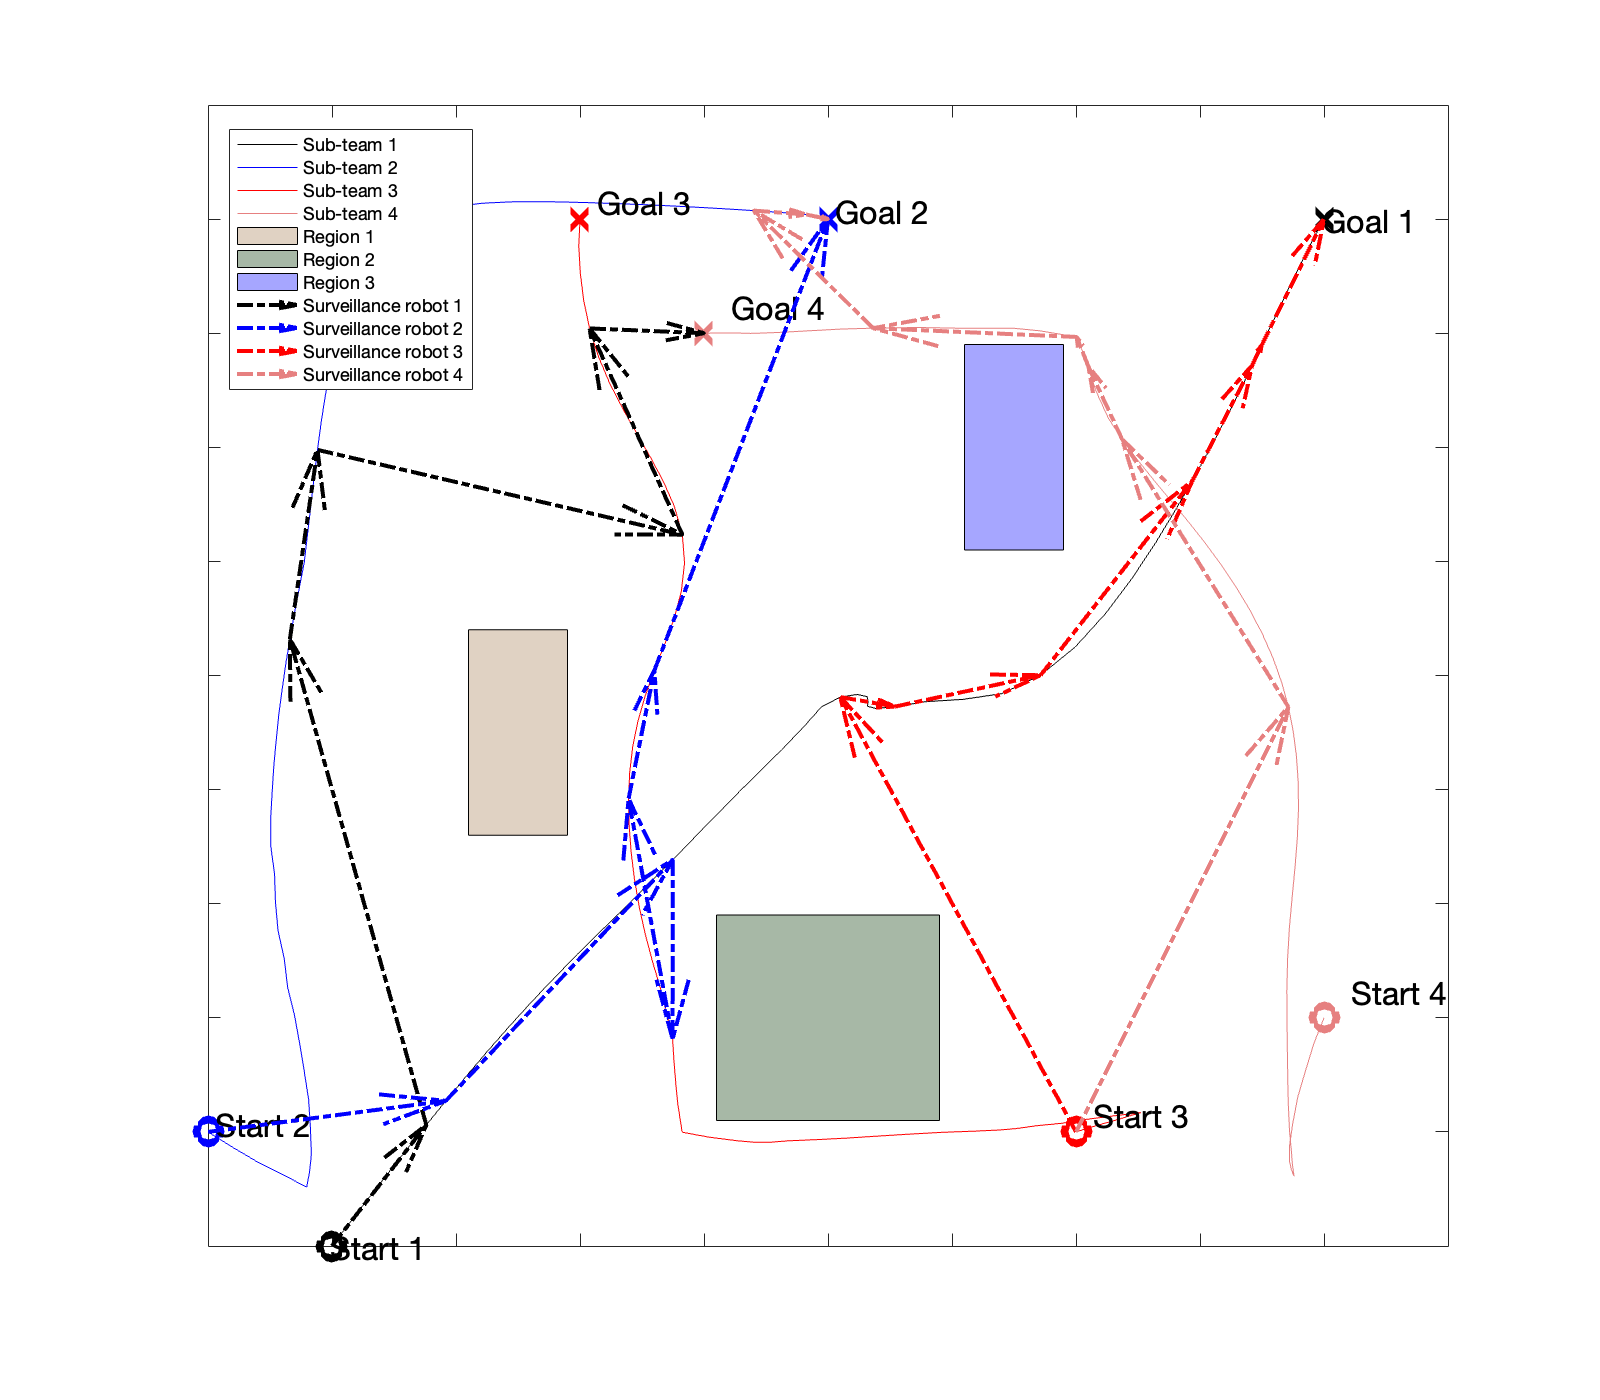
\includegraphics[width=0.47\linewidth,trim = 4cm 2cm 4cm 2cm, clip,valign=c]{Traj_result}}
  %\subfloat[Graph flow result\label{fig:result-graph}]{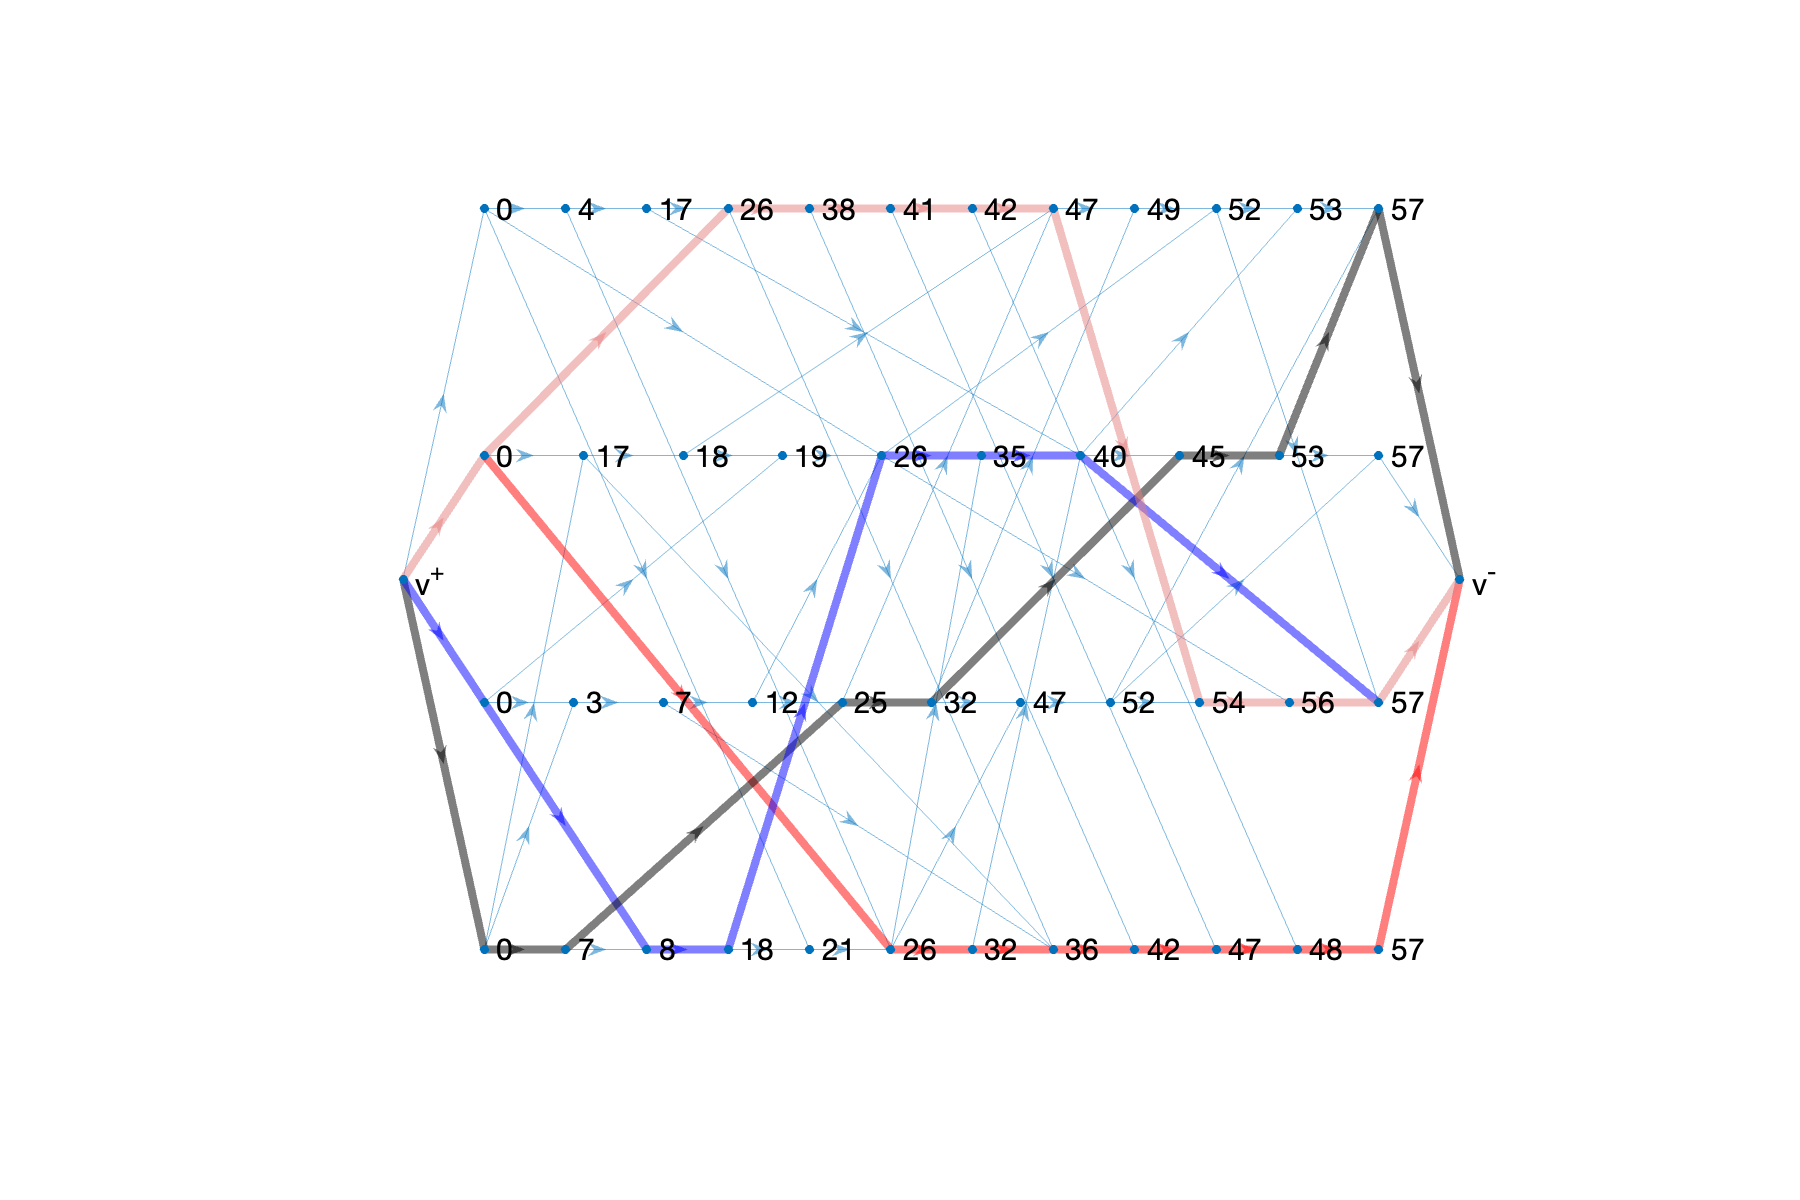
\includegraphics[width=0.47\linewidth,trim = 4cm 0cm 4cm 0cm, clip,valign=c]{Graph_result}}
  \subfloat[7-agent co-observation plan\label{fig:Result-plan-7-team}]{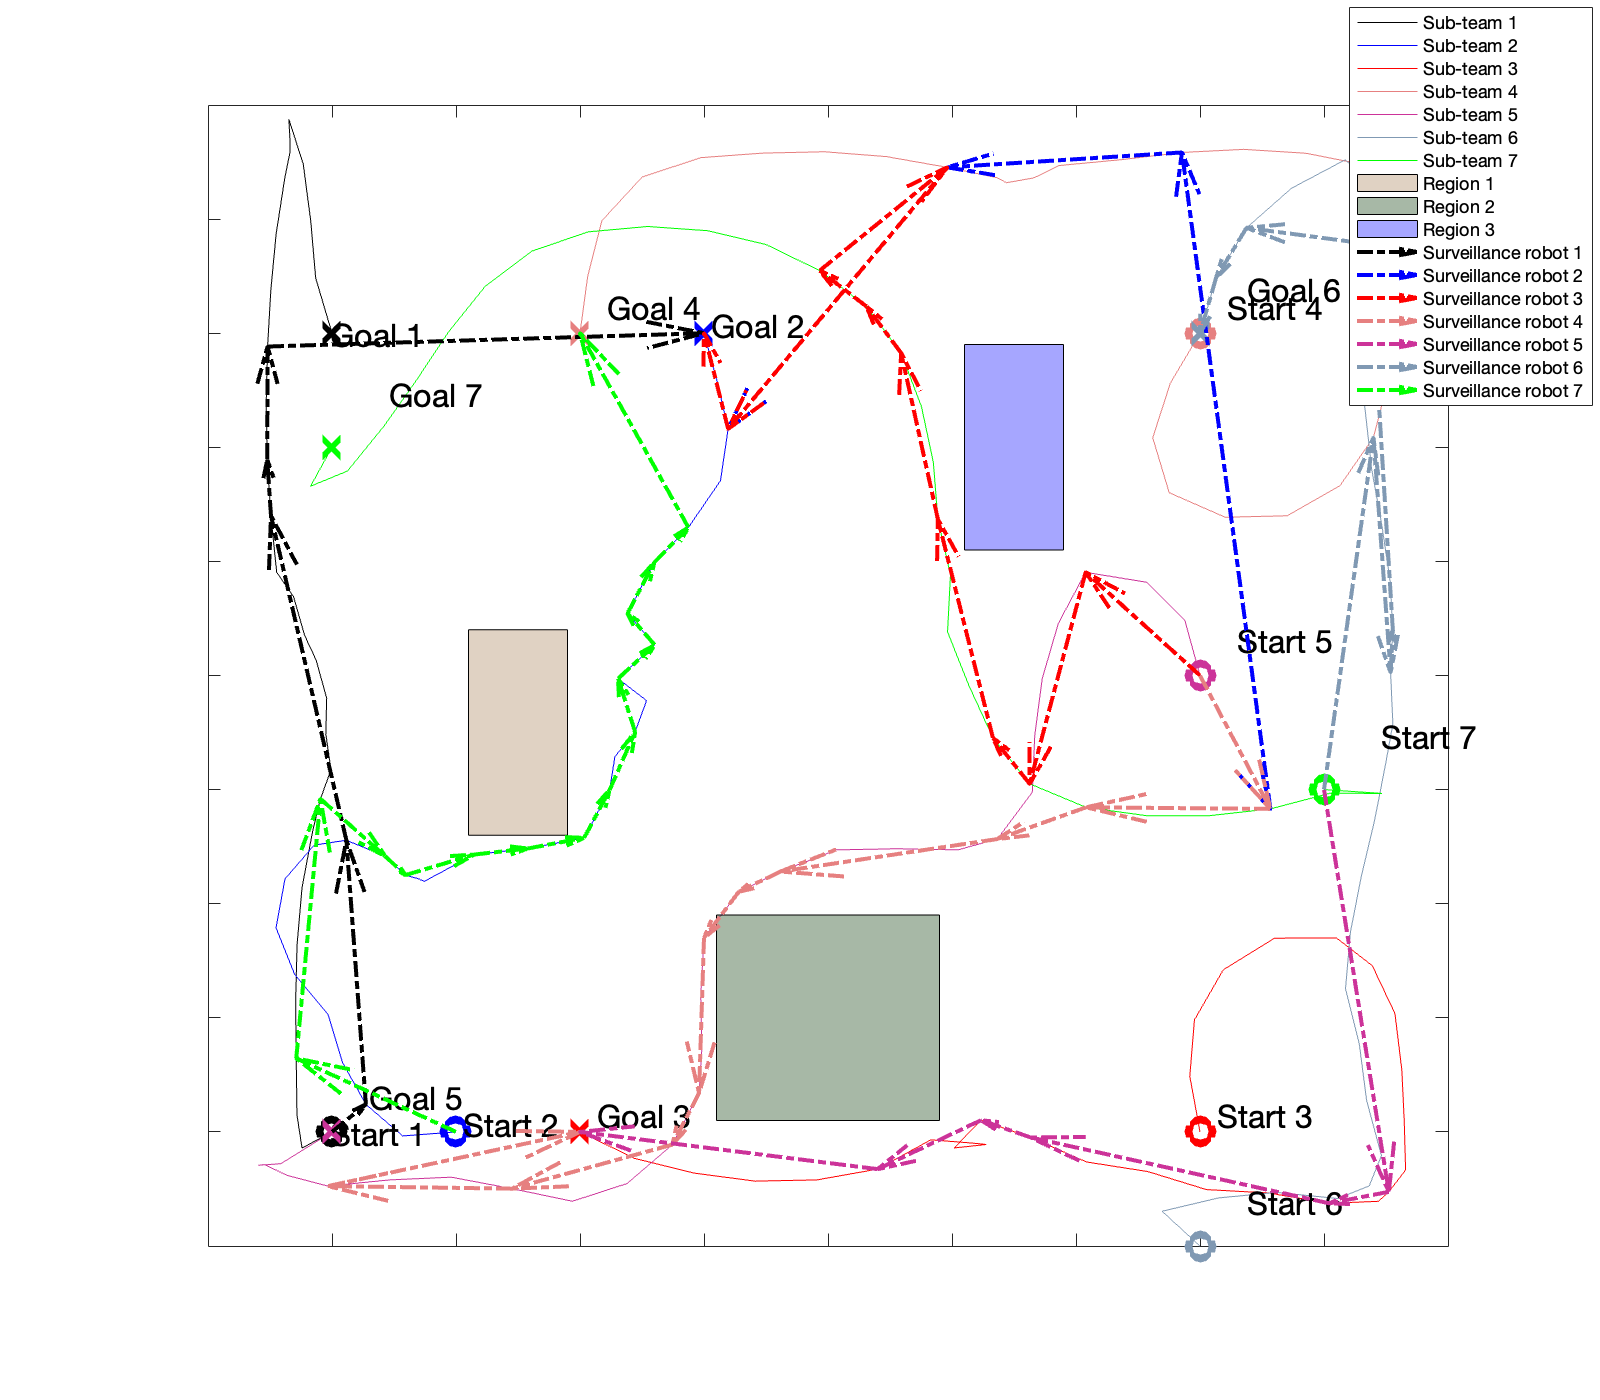
\includegraphics[width=0.47\linewidth,trim = 4cm 2cm 4cm 2cm, clip,valign=c]{7-team-plan.png}}
  %\subfloat[Graph flow result\label{fig:result-graph-7-team}]{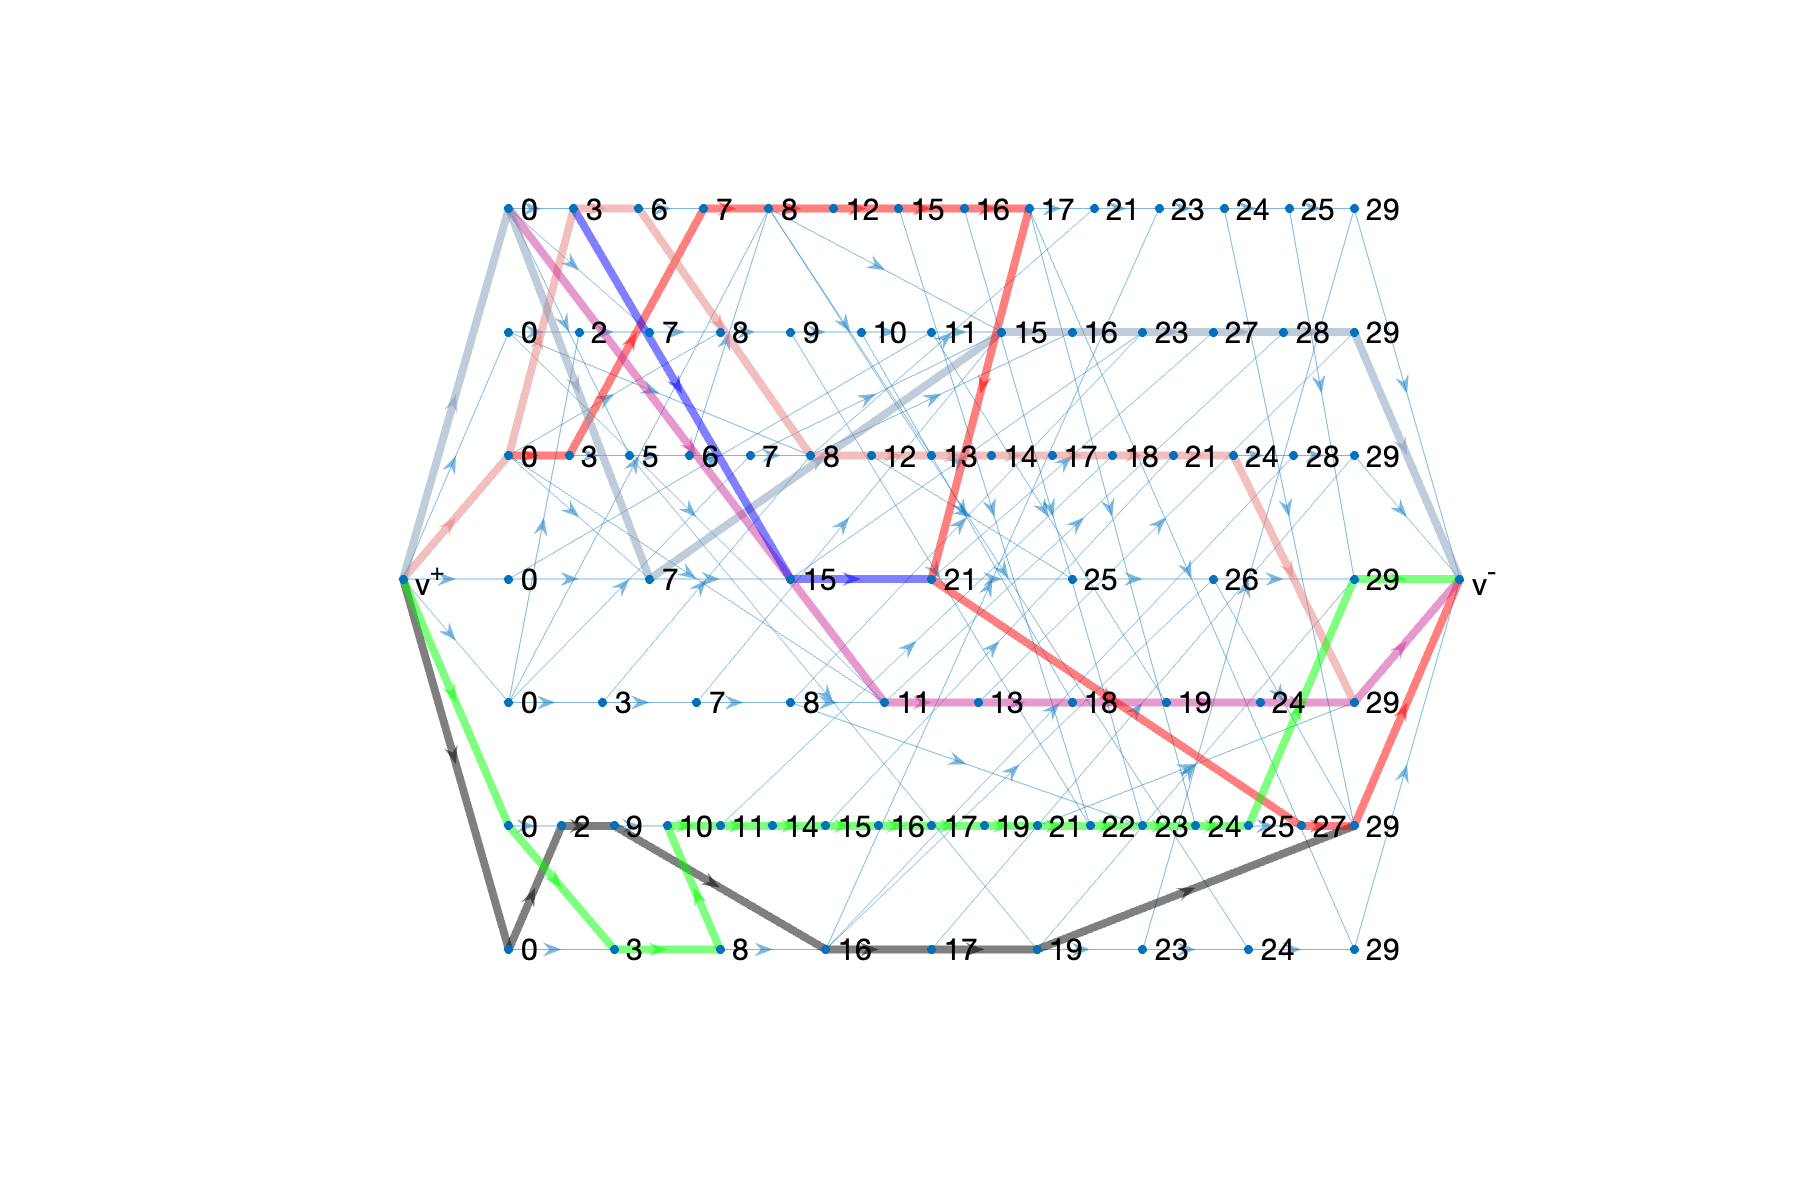
\includegraphics[width=0.47\linewidth,trim = 4cm 0cm 4cm 0cm, clip,valign=c]{7-team-graph.png}}
  \caption{Cross-trajectory co-observation result of a 4 sub-teams task (\Cref{fig:Result-plan}) and a 7 sub-teams task \Cref{fig:Result-plan-7-team}}\label{fig:Cross-trajectory-result}
\end{figure}

% \begin{figure}
%   \centering
%    \subfloat[Cross-trajectory co-observation plan\label{fig:Result-plan-7-team}]{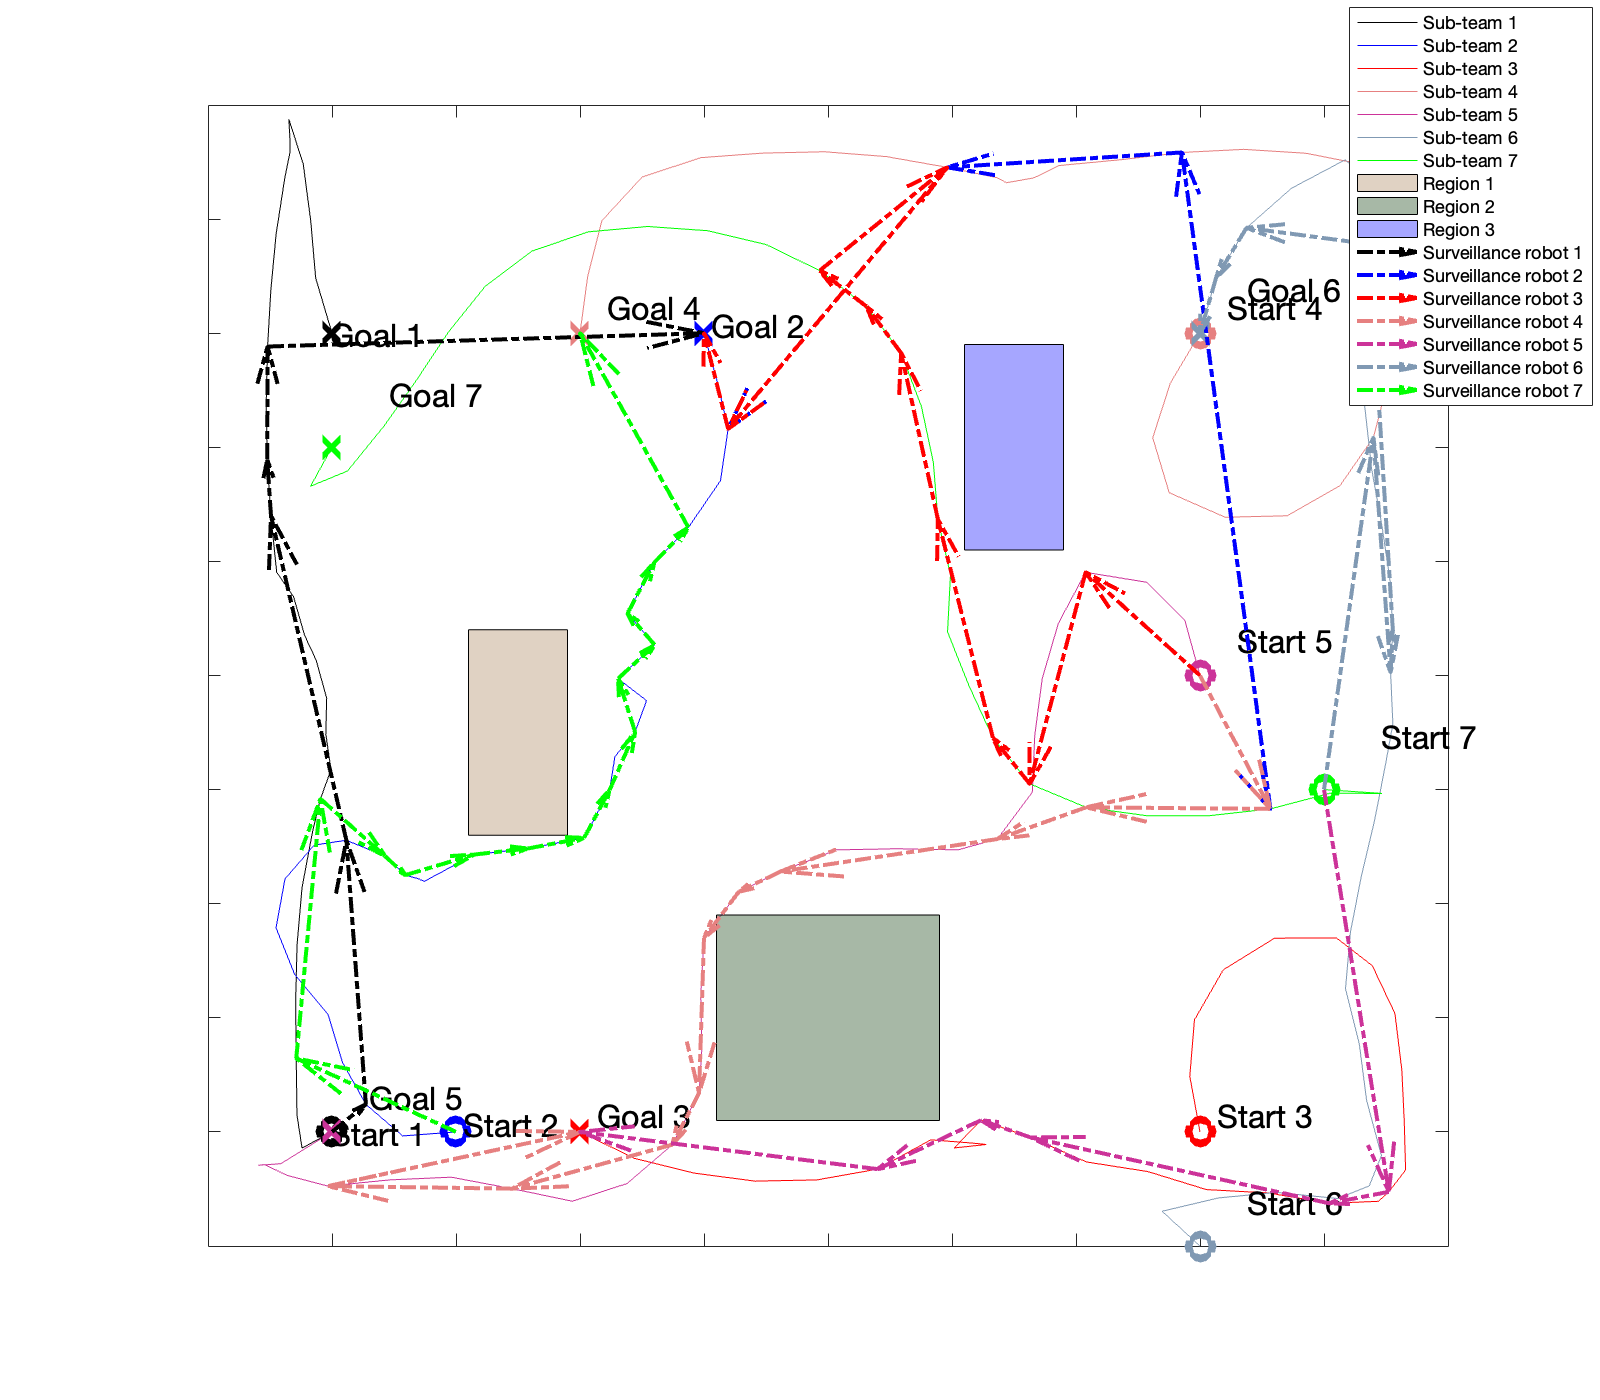
\includegraphics[width=0.47\linewidth,trim = 4cm 2cm 4cm 2cm, clip,valign=c]{7-team-plan.png}}
%   \subfloat[Graph flow result\label{fig:result-graph-7-team}]{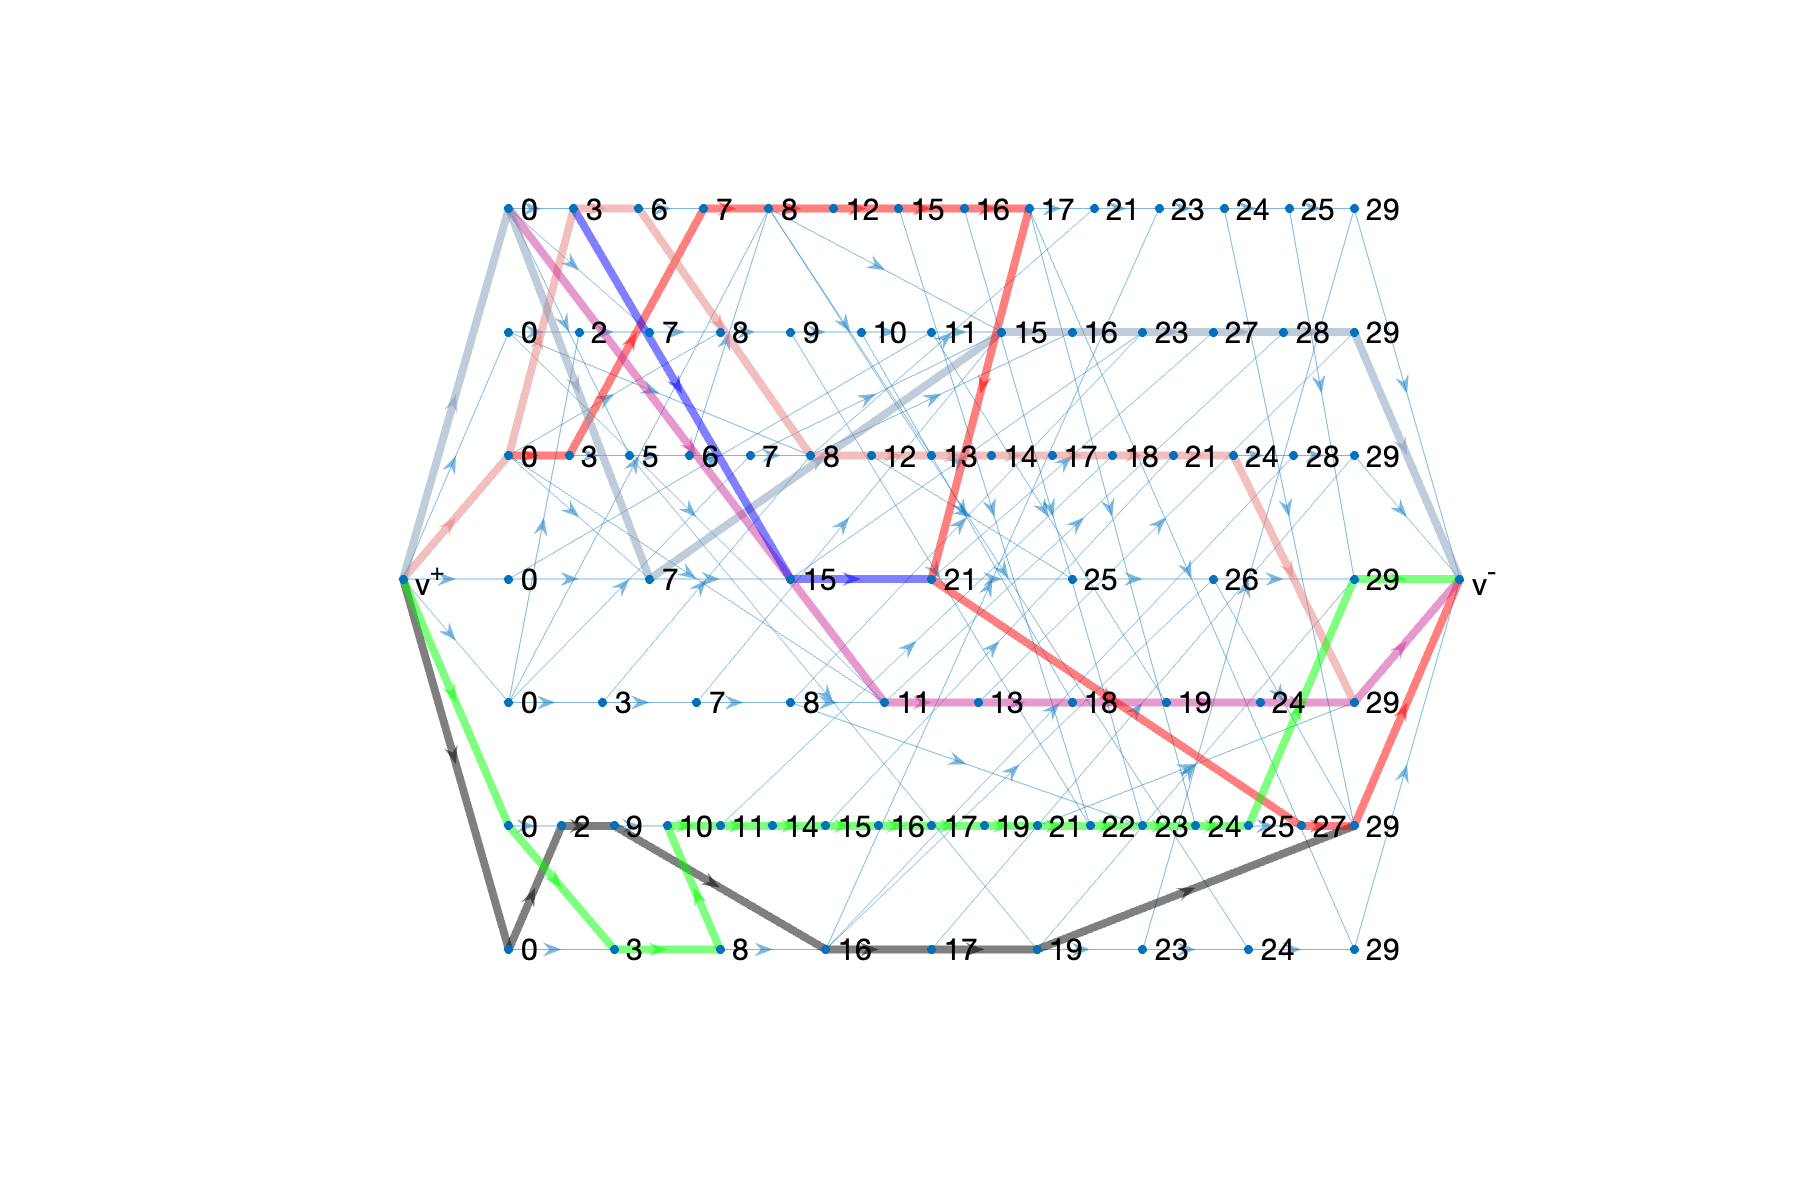
\includegraphics[width=0.47\linewidth,trim = 4cm 0cm 4cm 0cm, clip,valign=c]{7-team-graph.png}}
%   \caption{Cross-trajectory co-observation result of a 7 sub-teams task.}\label{fig:Cross-trajectory-result-7}
% \end{figure}

\section{Summary}\label{sec:summary}
This paper introduces security measures to protect Multi-Robot Systems (MRS) from plan-deviation attacks. By incorporating co-observation schedules and ensuring the reachability of robots during unobserved periods avoid forbidden regions, we present a secured trajectory optimized for specific scenarios. This guarantees that any deviations into forbidden regions will break the schedule and trigger detection. In scenarios where a secured plan is infeasible or better task performance is needed, we propose the use of redundant robots for cross-trajectory co-observations. We formulate the co-observation plan for the redundant robots by solving a network flow coverage problem on the checkpoint graph generated from the original unsecured MRS trajectories, providing the same security guarantees against plan-deviation attacks.

However, given the time-sensitive nature of co-observation and the need for close proximity, collision avoidance during co-observation planning becomes crucial. Future work will focus on integrating collision avoidance into the planning phase. Additionally, dynamic assignment of duties within sub-teams will be explored, making it more challenging for attackers to plan and execute successful attacks. Real-time task assignment and control will be a key area of investigation

%In this paper, we provide methods to enhance the security of a MRS against plan-deviation attacks. First, by introducing co-observation schedule and keeping reachability region during unobserved periods away from the forbidden regions, we provide an secured trajectory optimized for certain scenarios with guarantees that any deviations to forbidden regions will for sure break the schedule and get detected. Additionally, for scenarios that requires better task performance or when a secured plan is not feasible, we introduce redundant robots to performs cross-trajectory co-observations that can provide any unsecured MRS trajectories with the same security guarantee.

%As co-observation is time-sensitive and requires robots to be in close proximity, it is important to consider the possible collision during co-observation planning. The main future work will focus on including collision avoidance in the planning phase. Additionally, the assignment of the duties within the sub-team can performed dynamically, making it more difficult for attackers to successfully plan and execute attacks. This makes realtime task assignment and control another topic worth looking into.

\appendix
\subsection{Proof of proposition \ref{prop:HProperty}} \label{proof:HProperty}
    For subclaim~\ref{it:orthonormality}:
    \begin{equation}
      H\transpose H=H^2=4uu\transpose u u\transpose - 4uu\transpose +I^2=I,
    \end{equation}
    since $u\transpose u=1$.

    For subclaim~\ref{it:determinant}, let $U=\bmat{u & u^\bot_{1},u^\bot_{2}}$, where $u^\bot_{1},u^\bot_{2}$ are two orthonormal vectors such that $I=UU\transpose=uu\transpose + u^\bot_{1}(u^\bot_{1})\transpose+u^\bot_{2}(u^\bot_{2})\transpose$; then, substituting $I$ in \eqref{eq:H definition}, we have that the eigenvalue decomposition of $H$ is given by
    \begin{equation}
      H=U\diag(1,-1,-1) U\transpose.
    \end{equation}
    Since the determinant of a matrix is equal to the product of the eigenvalues, $\det(H)=1$.

    For subclaim~\ref{it:transformation}, first note that $Hu=2uu\transpose u - u=u$.
    It follows that the sum of $\nu_\cF$ and $\nu_\cE$ is invariant under $H$:
    \begin{equation}\label{equ:H(u1+u2)}
      H(\nu_\cF+\nu_\cE)=H u \norm{\nu_\cF+\nu_\cE}
      = u\norm{\nu_\cF+\nu_\cE} =\nu_\cF+\nu_\cE,
    \end{equation}
    and that their difference is flipped under $H$:
    \begin{equation}\label{equ:H(u1-u2)}
      H(\nu_\cF-\nu_\cE) = 2uu\transpose (\nu_\cF-\nu_\cE) - (\nu_\cF-\nu_\cE)^2 = -(\nu_\cF-\nu_\cE).
    \end{equation}
    Combining (\ref{equ:H(u1+u2)}) and (\ref{equ:H(u1-u2)}) we obtain
    \begin{equation}
      H\nu_\cF = \frac{1}{2}\bigl(H(\nu_\cF+\nu_\cE)+H(\nu_\cF-\nu_\cE)\bigr)
      = \nu_\cE
    \end{equation}

\subsection{Proof or proposition \ref{prop:Hderivitive}} \label{proof:Hderivitive}
    From the definition of $H$ in \eqref{eq:H definition}, we have
    \begin{equation} \label{equ:H_dot original}
      \dot H =   2(\dot u u\transpose + u \dot u\transpose)
    \end{equation}

    Recall that $\dot{u}=\frac{1}{\norm{u'}}(I-uu\transpose)\dot{u}'$ (see, for instance, \cite{Tron:Arxiv14}), which implies $(I-uu\transpose)\dot{u}'=\dot{u}'$. It follows that $\dot{u}$ flips sign under the action of $H\transpose$:
    \begin{multline}
      H\transpose \dot u = (2u u\transpose-I)\frac{ \left( I - u u\transpose \right) } {\left\|u'\right\|} \dot u' \\
      =\frac{1}{\norm{u'}} (2u u\transpose-I-2u u\transpose u u\transpose+u u\transpose)\dot{u}'\\
      = -\frac{1}{\norm{u'}} (I-u u\transpose)\dot u'
      = -\dot u
    \end{multline}

    Inserting $HH\transpose=I$ in (\ref{equ:H_dot original}), we have
    \begin{equation}
      \begin{split}
        \dot H =  &  2H H\transpose(\dot u u\transpose + u \dot u\transpose)
        =  2 H (-\dot u u\transpose + u \dot u\transpose)\\
        =  &  -2H [[u]_{\times} \dot u]_{\times} \\
        = &  -2 H \left[ [u]_{\times}  \frac{ \left( I - u u\transpose \right) \left( I- \nu_\cF \nu_\cF\transpose \right)} {\left\|u'\right\| \left\|\nu_\cF\right\|} \dot{\nu}_\cF\right]_{\times}\\
        = & -2 H \cross{M \dot{\nu}_\cF},
      \end{split}
    \end{equation}
    which is equivalent to the claim.
  
  \subsection{Proof of proposition \ref{prop:Ellipse2PointDiff}}\label{proof:Ellipse2PointDiff}
      To make the notation more compact, we will use $\partial_q f$ instead of $\partial_{\left[\begin{smallmatrix}q_1\\q_2\end{smallmatrix}\right]} f$ for the remainder of the proof.
    The differential of \eqref{equ:Point2EllipseProjection} can be represented as:
    \begin{equation}\label{equ:dPi_dt}
      \begin{split}
        \dot \pi_{p\cE} = &  \dot H^{-1}SH (q_{avoid} - o)  + H^{-1}\dot S H (q_{avoid} - o) \\
        &+ H^{-1}S \dot H (q_{avoid} - o) + (H^{-1}SH -I)\dot o\\
      \end{split}
    \end{equation}

    where
    \begin{equation}\label{equ:S_dot}
      \begin{split}
        \dot S  =& - S^2 (Q \dot s + s \dot Q)\\
        =& - S^2 (Q \partial_q s \dot q - \partial_b Q \partial_q b \dot q)
      \end{split}
    \end{equation}
    where
    \begin{equation}
      \partial_b Q = 2\frac{s}{b^3} \diag\{0,1,1\}
    \end{equation}
    To compute the derivative $\partial_q \pi$, we need the expression of $\partial_q b$, $\partial_q o$ and $\partial_q s$; the first two can be easily derived using the equations above:
    \begin{align}
      \partial_q b &= \frac{1}{4b}\bmat{q_1-q_2,q_2-q_1}\transpose\\
      \partial_q o &= \bmat{I/2,I/2}\transpose
    \end{align}

    In order to get $\partial_q s$, we use the fact that $F\bigl(s(q)\bigr)=0$ for all $q$; hence $F\bigl(\tilde{q}(t)\bigr)\equiv 0$, and $\partial_q F = 0$. We then have:

    \begin{equation}
      0=\dot F =  2q\transpose Q' \dot q + q\transpose \partial_s Q' q \dot s + q\transpose \partial_bQ' q \dot b
    \end{equation}
    where
    \begin{equation}
      \partial_s Q'= -\diag\left(\frac{2a^2}{(s+a^2)^3},\frac{2b^2}{(s+b^2)^3},\frac{2b^2}{(s+b^2)^3}\right).
    \end{equation}
    By moving term $\dot s$ to the left-hand side we can obtain:
    \begin{multline}\label{equ:s_dot}
      \dot s =  (q\transpose \partial_s Q' q)^{-1} (2q\transpose Q' \dot q + q\transpose \partial_b Q' q \dot b)\\
      =  (q\transpose \partial_s Q' q)^{-1} (-4q\transpose Q' H[U\dot q]_\times (q_{avoid} - o) \\
      -2q\transpose Q'H\dot o + q\transpose \partial_b Q' q \dot b)\\
      =  (q\transpose \partial_s Q' q)^{-1} (-4q\transpose Q' H[q_{avoid} - o]_\times U\dot q \\
      -2q\transpose Q'H\dot o + q\transpose \partial_b Q' q \dot b)
    \end{multline}

    The second term of equation (\ref{equ:dPi_dt}) turns into:
    \begin{multline}
      H^{-1}\dot S H (q_{avoid} - o)
      = - H^{-1} Q' q \dot s - s H^{-1} S^2 \partial_b Q q \dot b\\
      =   \big( (q\transpose \partial_s Q' q)^{-1} H^{-1} Q' q q\transpose  (4Q' H[q_{avoid} - o]_\times U  \\
      + 2Q' H\partial_q o - \partial_b Q' q q \partial_q b) -  s H^{-1} S^2 \partial_b Q q \partial_q b\big) \dot q\\
    \end{multline}

    Thus equation \eqref{equ:dPi_dt} could be written as:
    \begin{multline}
      \dot \pi_{p\cE} = \big(-2 H [ SH(q_{avoid}-o)]_{\times}U   \\
      + \left( (q\transpose \partial_s Q' q)^{-1} H^{-1} Q' q q\transpose  (4Q' H[q_{avoid} - o]_\times U \right. \\
      \left.+ 2Q' H\partial_q o - \partial_b Q' q q \partial_q b) -  s H^{-1} S^2 \partial_b Q q \partial_q b\right) \\
      -2H^{-1} S H[q_{avoid}-o]_{\times} U  \\
      + (H^{-1}SH -I)\partial_q o \big) \dot q,
    \end{multline}
    from which the claim follows.
  
  \subsection{Proof of proposition \ref{prop:dpi_ne_dt}}\label{proof:dpi_ne_dt}
    We first need to derive $\dot{d}_\cE$ and $\dot{d}_{\cE t}$

    \begin{equation}
      \dot d_\cE = -n\transpose \partial_q o \dot q
    \end{equation}
    \begin{equation}\label{equ:dot det}
      \begin{split}
        \dot d_{\cE t} =&  (\dot n_\cE\transpose Q^{-1} n_\cE + n_\cE\transpose \dot Q^{-1} n_\cE + n_\cE\transpose Q^{-1} \dot n_\cE) /\sqrt{n_\cE\transpose Q^{-1} n_\cE}\\
        = & (\sqrt{n_\cE\transpose Q^{-1} n_\cE})^{-1}\left(-2n\transpose H[Q^{-1}n_\cE]_\times U \right.\\
        &\left. + n_\cE \transpose \partial_b Q^{-1} n_\cE \partial_q b  -2 n_\cE Q^{-1}H[n]_\times U \right) \dot q
      \end{split}
    \end{equation}
    Next, we need to derive  $\dot p_{t1}$, $\dot p_{t2} $ and $\dot p_\cL$. Since $p_\cL$ could be written as
    \begin{equation}
      p_\cL = \frac{d_\cE Q^{-1} n_\cE}{ d_{\cE t} ^2},
    \end{equation}
    we have
    \begin{multline}\label{equ:dpl_dt}
        \dot p_\cL =  \left( (-\frac{d_{\cE t} n\transpose \partial_q o -2d_\cE \partial_q d_{\cE t}}{d_{\cE t}^3} )Q^{-1}n_\cE \right.\\
        \left .+ \frac{d_\cE\partial_b Q^{-1} n_\cE \partial_q b -  2d_\cE Q^{-1}H[n]_\times U}{d_{\cE t}^2}\right) \dot q
    \end{multline}
    \begin{multline}\label{equ:dplt_dt}
        \dot p_{1} =  \left(-\frac{Q^{-1}n_\cE \partial_q d_{\cE t} }{d_{\cE t}^2} \right.\\
         \left. + \frac{\partial_b Q^{-1}n_\cE \partial_q b -  2Q^{-1}H[n]_\times U }{d_{\cE t}} \right) \dot q
    \end{multline}
    subtracting $\dot q$ from (\ref{equ:dpl_dt}) and (\ref{equ:dplt_dt}), we can derive the result shown in (\ref{equ:ProjectPoint})


{\small
\bibliographystyle{unsrt}
\bibliography{ADMM_planning,ACC,tron,ziqi,reachability}
}

\end{document}
